


随着边缘计算和人工智能技术的快速发展,将AI推理能力部署到边缘设备成为实现云边协同实时决策的关键需求,其核心优势在于通过云端全局调度与边缘本地化执行降低端到端延迟。然而,现有基于KubeEdge的AI推理系统存在显著不足:缺乏对设备管理机制动态感知能力、混合负载场景下资源调度僵化,以及边缘异构硬件适配成本高。

为解决上述问题,本文提出一种基于KubeEdge和Akka的分布式AI推理平台,通过逻辑-物理双层集群架构实现云端-边端的协同优化。本文主要贡献为:

\begin{itemize} 

\item 通过离线阶段构建节点推理性能预测模型,构建节点算力画像,在线阶段融合实时网络状态与设备负载特征,构建多目标优化函数,实现动态资源感知调度算法。设计高度可扩展的调度框架,支持动态添加优化目标与切换优化策略,可灵活应对不同场景下的优化需求。提出流式数据分片与并行处理机制,根据边缘节点算力动态调整并行处理粒度,在保证实时性的前提下最小化网络带宽占用,实现模型部署位置决策与数据流分片策略的联合优化。
\item 基于Akka Actor模型设计分布式架构,设计设备接入、资源调度与模型服务的分层接口规范。云端Master通过K8s Informer机制实时捕获设备状态变化,根据Worker原型动态生成符合条件的Worker负载;边端Manager基于可插拔接口实现Worker实例的弹性扩缩与任务优先级调度,开发者通过实现标准化接口可快速集成新型边缘设备与处理逻辑。
\item 设计云端统一模型仓库实现AI模型的版本化管理,基于硬件特征检测自动生成适配节点架构的负载容器,通过边缘侧插件化机制实现多推理引擎的模型服务的动态加载与热更新,显著降低异构硬件适配成本。
\end{itemize}



\begin{itemize} 
\item \textbf{响应时间}:深度学习应用的响应时间由计算延迟和通信延迟共同决定,其中计算延迟与模型规模和可用算力等因素相关;而通信延迟则受当前通信技术所限。由于广域网最初旨在提高带宽容量与链路效率,在大规模数据传输时不可避免地会出现高延迟、网络拥塞和不稳定等问题。
\item \textbf{数据安全和隐私}:传统云计算往往将数据传输到云端进行存储与分析,但加解密的高成本在一定程度上阻碍了其广泛应用。此外,随着数据隐私和安全意识提升,去中心化并在可行的情况下强调在数据源处或附近进行处理变得至关重要。
\end{itemize}


在这种传统模式下,深度学习应用的响应时间受到计算延迟和通信延迟的共同影响,其中计算延迟与模型规模和可用算力等因素密切相关,而通信延迟则受限于当前的通信技术。由于广域网最初设计是为了提升带宽容量和链路效率,处理大规模数据时会不可避免地产生高延迟、网络拥塞等问题,导致通信延迟显著增加。此外,传统云计算往往将数据传输到云端进行存储与分析,但加解密的高成本阻碍了其广泛应用,且随着对数据隐私和安全性的关注增加,去中心化处理逐渐成为一种趋势,尤其是在数据源附近进行本地处理显得尤为重要。


中发挥着至关重要的作用。云计算可将云端服务器的强大算力赋能给性能有限的终端设备,使其同样能够获取高效的计算与存储服务\cite{shafi20175g}。然而在传统的云计算范式下,数据需要传输到中心数据中心进行处理,这在带宽需求高的场景中会造成显著的网络负载,逐渐难以满足这些应用场景对服务质量(Quality of Service, QoS)的要求\cite{wang2024end}。


为应对上述挑战,将深度学习模型部署到更贴近数据源的边缘节点成为一种可行的解决方案,即边缘计算。与传统云计算不同,边缘计算则将计算任务下放至网络边缘,减少了数据的回传时间和带宽消耗,从而缩短数据传输距离和响应时间,显著提高了应用的实时响应能力,同时增强数据隐私\cite{chowdhury2019co,khan2019edge,liu2019survey,施巍松2019边缘计算,刘通2021边缘计算中任务卸载研究综述}。然而,边缘端的性能受到硬件资源和能耗等方面的限制。虽然可以采用一些轻量级模型以降低计算和存储需求,但这往往会牺牲一定的\textbf{模型准确率},使其难以满足某些对系统可靠性要求较高的应用场景。在这种情况下,需将计算请求转发至云端或其他具备足够资源的边缘端进行处理。由此可见,云端和边缘端的协同工作,即云边协同,是应对各个场景需求的关键。




为应对这些挑战,学术界也探索了计算卸载策略。例如,Urgaonkar等人\cite{urgaonkar2015dynamic}将负载调度问题建模为马尔可夫决策过程,并结合李雅普诺夫优化,使调度算法能够根据当前系统负载进行实时调整,从而在不确定条件下保持系统的稳定性与高效性。Han 等人\cite{han2019ondisc}等人提出了一种名为 OnDisc 的在线负载调度与卸载算法,在单个节点上定义了残余密度(Residual Density)的度量,通过“最高残余密度优先”来满足对延迟敏感的负载需求;在多节点场景中,OnDisc 通过最小化计算卸载所带来的总加权响应时间来进一步降低整体延迟。Meng等人\cite{meng2019online}则提出名为 Dedas 的在线负载调度和卸载算法,量化网络带宽对传输时延的影响,并引入了“截至期限”(Deadline)的概念,在单节点内使用最早截止期限优先调度策略,在多节点间则通过最小化负载完成时间来实现高效的卸载与调度。此外,部分研究\cite{崔玉亚2021一种面向移动边缘计算的多用户细粒度任务卸载调度方法,邝祝芳2022基于深度强化学习的多用户边缘计算任务卸载调度与资源分配算法,郑守建2022一种基于综合匹配度的边缘计算系统任务调度方法,张斐斐2023边缘计算中协作计算卸载与动态任务调度}还借助启发式策略或强化学习方法设计调度算法,以进一步提升调度效率和系统性能。

然而,以上工作均针对通用计算负载,仅考虑时延对服务质量的影响,未能充分考虑深度学习应用中准确率对系统性能的影响。这一局限性限制了现有调度算法在需要高精度计算的深度学习场景中的应用效果,无法全面优化系统的资源分配和整体性能。针对这一问题,Salem 等人\cite{salem2023toward}提出了推理交付网络(Inference Delivery Network,IDN)的概念,旨在解决机器学习模型在设备端与云端部署时面临的延迟与准确性之间的权衡。同时,他们提出了一种名为 INFIDA 的模型分配分布式动态策略,采用在线镜像上升(Online Mirror Ascent,OMA)的方法加速收敛,并有效应对非凸决策空间和复杂成本函数。然而,Salem 等人的研究未能充分考虑如何根据实时变化的应用场景动态调整深度学习模型在云端和边缘节点之间的部署位置,导致其在适应动态服务质量需求方面表现不佳。例如,当某些节点出现异常或即将发生故障时,为了及时采取措施避免生产中断,模型推理的延迟要求可能会急剧提高,而准确性要求则可能在一定程度上有所降低。


当前研究提出了多种方法,包括端到端实际测量、基于浮点运算量(FLOPs)的轻量级预测以及基于硬件感知的建模方法(如 nn-Meter)。

对于深度学习推理来说,模型的计算需求必须适配目标设备的硬件特性,但异构环境下的适配和模型迁移需要对任务进行细粒度划分和动态调整,从而大幅增加了调度的复杂性。在边缘端,评估深度学习推理性能的关键指标是推理时延。传统的基于测量的方法需要复杂的部署过程,尤其在多样化的边缘设备和推理框架场景下,难以应对设备数量的快速增长。现有的基于FLOPs的方法在预测准确性上存在不足,无法满足实际需求。


深度学习模型通过训练实现推理功能,即通过学习大规模数据提取特征并优化参数,从而在推理阶段快速生成预测结果。模型训练因其计算和 I/O 密集性长期是研究优化的重点,而推理虽无需复杂迭代算法,通常被认为较为简单。然而,随着深度学习应用的快速发展,推理不仅需要满足更高的实时性要求,还需应对海量传感设备带来的急剧增长需求,这对系统性能和资源分配提出了严峻挑战。

目前,深度学习推理服务主要有两种方式:一是通过边缘设备运行简单模型提供服务;二是依托远程云基础设施,通过“机器学习即服务”(MLaaS)平台运行复杂模型,以高吞吐量支持推理。然而,这两种方式在某些场景下存在局限性——边缘设备的模型难以满足精度需求,而云服务则无法达到严格的低延迟要求。在此背景下,云边协同计算通过结合云与边缘的优势,利用智能资源编排和优化调度机制,在性能与延迟之间实现有效权衡,在深度学习模型调度中发挥了重要作用。

尽管如此,目前大多数推理服务解决方案,如 TensorFlow Serving\cite{olston2017tensorflow} 和 Azure ML\cite{chappell2015introducing},主要面向云端推理服务的供应问题。然而,这些解决方案在应对复杂推理需求和多样化应用时存在一定局限性,尤其是在延迟和吞吐量方面。为了解决这些问题,Crankshaw 等人\cite{crankshaw2017clipper} 提出了 Clipper 系统。Clipper 通过实现预测缓存,减少了频繁查询带来的延迟和系统负载,并利用自适应批处理技术,根据模型容器的延迟配置文件动态调整批处理大小,从而优化了吞吐量与延迟之间的平衡。Clipper 还通过模型抽象层简化了不同机器学习框架之间的差异,使得开发者能够专注于模型的部署和优化,而无需关注底层框架的选择。在此基础上,Crankshaw 等人\cite{crankshaw2020inferline}提出了 InferLine,一个用于配置和管理机器学习推理管道的系统。InferLine 专注于在异构并行硬件上以低成本满足端到端延迟要求,系统通过为每个模型创建性能配置文件并估算管道的端到端延迟,优化了管道的资源分配。它还能根据实际工作负载的变化,动态调整管道配置,在负载增加时自动扩展副本数,并在负载减小时根据最小供应比率缩减副本数,从而确保系统始终满足延迟和吞吐量要求。此外,Mao 等人\cite{mao2019learning} 提出了名为 Decima 的架构,基于强化学习调度策略,可以在无需人工输入复杂调度算法的情况下,根据不同工作负载和环境条件自动学习最优策略,从而提高集群资源的利用率。然而,以上这些解决方案主要解决了云端推理服务的供应问题,并未充分考虑边缘端节点的特殊需求,尤其是在小型集群和网络延迟至关重要的地理分布式基础设施中。例如,这些方案都没有考虑不同计算节点之间的网络延迟,而在云端部署环境中,网络延迟往往可以忽略不计。

针对边缘端推理服务供应问题,目前相关研究仍然较少。一些研究提出了模型拆分技术,通过将深度学习模型的执行分布到多个离散计算单元上,以适应移动硬件平台的资源限制。Lane 等人\cite{lane2016deepx} 提出了 DeepX 框架,专注于优化深度学习模型在移动设备上的推理性能。该框架通过运行时层压缩(RLC)和深度架构分解(DAD)两种核心算法有效缓解了移动设备资源受限的难题。RLC 方法利用奇异值分解(SVD)对模型权重进行压缩,显著降低计算量和内存占用,同时通过引入估计器控制压缩程度,确保模型准确性保持在可接受范围内。DAD 方法则通过将复杂的深度模型分解为多个单元块,并将其分配到本地和远程处理器上,最大化资源利用效率。在推理过程中,这些单元块的计算结果会被重组,生成最终的预测输出。此外,Teerapittayanon 等人\cite{teerapittayanon2017distributed} 提出了分布式深度神经网络(DDNN)架构,以应对分布式计算层次结构上运行深度神经网络(DNN)时的诸多挑战。DDNN 架构通过将训练好的 DNN 映射到本地、边缘和云端的异构物理设备上,有效解决了设备资源受限和通信成本过高的问题。然而,模型拆分技术与本文研究的模型调度方法是正交的,两者各自解决不同层面的问题,为未来进一步结合两种技术提供了可能性。这种结合可以为边缘计算场景下的深度学习推理服务提供更高效、更灵活的解决方案。

这一方法显著降低了数据采样成本,同时大幅提高了预测准确性。在 nn-Meter 工具的基础上,本文进一步对其进行了改进,使其适配云原生环境,能够在不同资源隔离策略下进行推理时延预测。通过这些改进,系统不仅能够满足多样化边缘设备的性能评估需求,还能够更好地支持云边协同环境下的推理任务优化。

因此,将AI推理能力部署到边缘设备并实现云边协同,成为满足实时决策需求的关键。然而,现有云边协同AI推理系统在动态资源调度和异构设备适配等方面存在显著不足。例如,传统调度方法难以根据实时网络状态和设备负载动态优化资源分配,而边缘设备的硬件异构性进一步增加了系统设计的复杂性。此外,模型版本管理、任务优先级调度等问题也对系统的性能和稳定性提出了挑战。云边协同通过云端全局调度与边缘本地化执行相结合,能够有效降低端到端延迟,但在实际部署中仍需解决资源分配效率低、系统适应性不足等问题。

基于此,本文提出一种基于KubeEdge和Akka的分布式AI推理平台,旨在通过逻辑-物理双层集群架构实现云端与边缘端的协同优化。研究聚焦于云边协同环境下AI推理服务的优化,具体包括以下方向:

综上所述,在云边协同计算模式下,合理分配计算资源以平衡模型的准确性、响应延时和资源利用率,并将深度学习模型部署到适当的节点以满足特定应用需求,仍然是一个具有挑战性的问题。本文聚焦于云边协同环境下的深度学习推理服务供应系统,旨在通过节点间的协作,优化服务质量指标的平衡,进而满足推理服务的多样化需求。具体的研究内容包括以下几个方面:

\begin{enumerate}
\item[1.] 如何在云端与边缘端之间选择最合适的部署位置,以满足服务质量指标的深度学习模型需求,实现不同层次之间的垂直协作,从而优化资源分配并提升整体系统性能。
\item[2.] 如何在同一层级的多个计算节点之间实现高效协作,例如边缘计算节点之间的协作,实现水平协作,进而提高系统的可扩展性、稳健性和负载均衡能力。
\end{enumerate}


云计算自诞生以来,通过虚拟化技术和大规模数据中心架构,为各行业提供了弹性且可扩展的资源共享模式。随后,容器化技术及微服务架构的引入,推动了云原生概念的兴起,进一步提升了云端系统的可移植性与交付效率\cite{deng2024cloud}。在此过程中,Kubernetes\cite{kubernetes}、Docker Swarm\cite{dockerswarm}等编排工具成为云原生生态的重要支柱,使大规模集群管理与自动化部署成为现实。基于这些先进的云端技术与架构,工业界开始将云的计算、网络与存储能力延伸至边缘侧,以满足低延时和高可靠性的应用需求,其中较为成熟的方案包括 Rancher 公司开发维护的 k3s\cite{fogli2021performance}、华为贡献给云原生基金会(CNCF)的 KubeEdge\cite{xiong2018extend} 以及阿里巴巴开源的 OpenYurt\cite{openyurt2023}。它们均依托于 Kubernetes 的容器编排与管理能力,在此基础上进行功能裁剪或扩展,满足边缘场景下的资源约束与分布式需求,同时提供了一定的边缘自治能力,使系统在网络不稳定或与云端短暂失联时仍能维持关键服务。

但是,当前的云边协同方案在高效调度方面仍存在一些不足:K3s 缺乏专门的云边协同组件,而 KubeEdge 和 OpenYurt 虽然引入了更精细的节点分组与管理功能,但其调度算法依然基于传统的云端任务分配逻辑,难以完全满足云边协同场景对低延迟和高可靠性的需求,尤其在部署位置的选择上仍有进一步优化的空间。经过综合评估,本系统研究最终选用 KubeEdge 作为底层架构。这主要基于以下考虑:首先,KubeEdge 从设计上原生支持云边协同,将“云-边-端”融为一体,提供丰富的边缘设备管理和数据处理能力,相较于缺乏云边协同组件的 K3s,它更适合大规模、多功能的边缘计算场景,同时相比 OpenYurt,它对边缘端资源的要求更低,且在设备管理方面表现更优;其次,作为 CNCF 项目,KubeEdge 拥有高活跃度的社区以及成熟的文档、示例和教程,能够在开发与运维阶段提供更完善的支持。

但是,这些方案在云边协同下的高效调度方面仍有不足:k3s 缺少专门的云边协同组件;KubeEdge 和 OpenYurt 虽然引入了更精细的节点分组与管理,但仍基于传统云端分配任务的调度算法,难以完全满足云边协同场景下对低延迟和高可靠性的需求,在部署位置的选择上仍存在优化空间。

综合评估后,本系统研究最终选用 KubeEdge 作为底层架构,主要基于以下考虑:

\begin{itemize} 
\item \textbf{云边协同的原生支持}:KubeEdge 从框架设计上就将“云-边-端”融为一体,提供丰富的边缘设备管理和数据处理能力。与缺乏云边协同组件的 k3s 相比,KubeEdge 更适合大规模、多功能的边缘计算场景;与 OpenYurt 相比,KubeEdge 对边缘端资源的要求更低,并在边缘设备管理上表现更佳。
\item \textbf{良好的社区生态与文档}:KubeEdge 作为 CNCF 项目,拥有高活跃度的社区和成熟的文档、示例及教程。与其他方案相比,它能够在开发与运维阶段提供更完善的支持。 
\end{itemize}

\item[3.] 如何在松散耦合的云边结构和较高的通信时延下实现资源的动态感知,以获取边缘节点的负载、带宽、计算能力等实时数据,确保云端能够在最佳时机做出快速响应并合理调度资源。

随着第五代移动通信技术(5G)的成熟和终端设备的迅速发展,推动了移动互联网交互式应用(如面部识别、地图导航等)的普及,这些应用为人们的生活和社会发展提供了极大的便利。这一趋势得益于云计算(Cloud Computing,CC)的广泛应用,使得性能有限的移动设备也能够享受到强大的计算和存储服务\cite{shafi20175g,zhang2010cloud}。

随着物联网(IoT)和云服务的快速发展,边缘计算逐渐成为一种新的计算模式,广泛应用于满足低延迟、节省带宽和增强数据安全的需求\cite{shi2016edge}。与传统的云计算相比,边缘计算具备更低的延迟和更强的位置感知能力\cite{mao2017survey,liu2019survey}。在云计算模式下,数据需要传输到中心数据中心进行处理,这在带宽需求高的场景中会造成显著的网络负载。而边缘计算则将计算任务下放至网络边缘,减少了数据的回传时间和带宽消耗,从而缩短数据传输距离和响应时间,显著提高了应用的实时响应能力\cite{shi2016edge,varghese2016challenges,khan2019edge}。

边缘计算在实践中已经被广泛应用于多种对实时性和带宽效率要求高的场景。例如,在城市监控和交通管理中,边缘计算可以帮助处理实时数据,以优化交通流量并提升公共安全\cite{yu2017survey};在工业生产中,它能够支持传感器数据的实时分析与反馈,从而促进生产流程的自动化和预测性维护\cite{liu2019survey};在智能家居系统中,边缘计算通过本地数据处理,既保护了用户隐私,又提升了设备的响应速度,从而带来更佳的用户体验\cite{yu2017survey}。图2-1展示了常见的边缘计算的应用场景。

\begin{figure}
    \centering
    \includegraphics[width=\linewidth]{pics/edge.png}
    \caption{边缘计算的应用场景}
    \label{fig:my_label}
\end{figure}

一个典型的边缘计算架构,共分为端-边-云三个层级,端层(End Layer)指的是物联网设备、传感器或终端用户设备,它们生成数据并可能执行一些简单的本地处理任务;边层(Edge Layer)通常是指接近数据源的边缘节点,如边缘服务器或网关,这些设备处理数据、执行计算任务,并与云端进行通信;云层(Cloud Layer)则是传统的云计算数据中心,提供强大的计算、存储和网络资源,用于处理需要大规模计算的任务,或者存储和管理大量数据。在端-边-云的边缘计算架构,边层节点的硬件资源呈现出高度的多样性,这种多样性即为边缘节点的异构性\cite{shi2016edge,yu2017survey}。图2-2展示了边缘计算架构和异构化的边层节点。

\begin{figure}[ht]
  \centering
  \includegraphics[width=\linewidth]{pics/2-2.png}
  \caption{边缘计算架构和异构化的边缘节点}
  \label{fig:my_label}
\end{figure}

\subsection{边缘节点的异构性}

边缘节点的异构性是指分布在边缘计算网络中的各类计算资源在性能、能效、存储容量和支持的任务类型等方面存在显著差异\cite{cooke2020model,varghese2021survey}。这些边缘设备包括低功耗的CPU、高并行处理能力的多核GPU,以及专用的AI加速器(如VPU)等硬件资源。异构化的边层节点使边缘计算系统能够根据任务的需求灵活选择最适合的硬件资源,从而提升整体计算效率\cite{varghese2020survey}。例如,在计算密集型的深度学习任务中,高性能的GPU或AI加速器能够显著减少推理时间;而对于实时性要求较高的任务,如自动驾驶和实时视频分析,边缘节点可以通过本地计算提供毫秒级的响应。然而,这种异构性也带来了系统设计和管理上的挑战。不同硬件架构的计算能力、功耗需求以及任务类型的兼容性差异,需要通过高效的调度算法和资源管理策略加以平衡,以确保系统在运行中的稳定性和高效性\cite{das2018edgebench}。

为了提高调度算法的精确度,异构化节点上对于不同负载的时延预测成为一项复杂的任务。Zhang\cite{zhang2021nn}等人提出了nn-Meter工具,该工具通过通过细粒度的内核分析,构建内核级延迟预测器,分析和预测不同边缘设备上的深度学习模型推理延迟。该工具能够支持多种硬件平台,如移动CPU、GPU和AI加速器,以应对边缘节点的多样化特性。但是,nn-Meter主要适配边层移动端的节点,其预测模型的泛化能力受限,不能应对更多动态环境下的边缘节点延迟问题。Li\cite{li2022inference}等人通过结合实时监控数据和模型自适应调整技术,开发了一种能够应对不同硬件配置和网络状态的预测框架,有效缓解了面对动态网络条件和硬件变化时,传统模型在异构节点上面临的泛化能力不足的问题。但是,实现和部署这样一个复杂的自适应预测系统需要较高的计算和存储开销,这在某些边缘设备上可能受到限制。

\subsection{边缘计算系统的调度算法}

在边缘计算系统中,如何高效调度和分配任务是实现系统性能优化的关键。调度算法在边缘计算中起到至关重要的作用,直接影响任务的响应时间、资源利用率和整体系统性能。由于边缘计算节点的异构性和任务的动态性,调度算法需要解决复杂的资源管理和任务分派问题,以满足延迟敏感应用和有限带宽环境下的需求。

Urgaonkar\cite{urgaonkar2015dynamic}等人提出了一种将工作负载调度问题建模为马尔可夫决策过程(Markov Decision Process,MDP)的方法,并使用李雅普诺夫优化(Lyapunov optimization)使得调度算法可以根据当前系统负载进行实时调整,从而在不确定性条件下维持系统的稳定性和高效性。Han\cite{han2019ondisc}等人提出了一种名为OnDisc的在线作业调度和调度算法,通过最高残余密度优先(Highest Residual Density First,HRDF)调度策略以及一种基于负载变化的分发策略,旨在最小化所有任务的总加权响应时间(Weighted Response Time,WRT)。Meng等人\cite{meng2019online}提出了一种名为Dedas的在线实时的任务调度与调度算法,该方法联合考虑了网络和计算资源的调度,通过贪心策略调度新到达的任务,并根据需要替换现有任务来满足新任务的截止时间,以最大限度满足任务截止期限。


为了评估 ,Cagatay\cite{sonmez2018edgecloudsim}等人提出了EdgeCloudSim,一个用于边缘计算系统性能评估的模拟环境。EdgeCloudSim专为研究和测试边缘计算场景中的调度算法和资源管理策略而设计,能够有效地模拟网络延迟、任务分配、数据传输和设备异构性等关键因素。EdgeCloudSim的多场景仿真功能,使研究人员能够在虚拟环境中测试和优化边缘计算系统,以便在实际部署中实现更高的效率和稳定性。




边缘计算范式通过将计算资源从中心化的数据中心迁移至网络边缘,提供了一种有效的解决方案,不仅能够有效缓解中心化数据中心的压力,还能够在本地处理数据,减少对网络带宽的依赖,提高数据处理的实时性和可靠性\cite{chowdhury2019co,khan2019edge,liu2019survey,施巍松2019边缘计算,刘通2021边缘计算中任务卸载研究综述}。与云计算相比,边缘计算有以下特性:


然而传统的集中式计算模式由于存在高延迟和高传输成本等问题,逐渐难以满足这些应用场景对服务质量(Quality of Service, QoS)的要求。这边的服务质量,不仅仅包括

已经广泛应用于生产生活的各个领域,

在这些需求中,AI视觉技术扮演着至关重要的角色。


在这些需求中,AI视觉技术扮演着至关重要的角色。例如,在智慧城市中,通过实时数据处理来优化交通流量、提高公共安全\cite{lin2016real,jia2017edge,mohamed2017smartcityware,mallapuram2017smart,dalla2017using};在工业生产中,通过对



然而,传统的集中式计算模式由于存在高延迟和高传输成本等问题,逐渐难以满足这些应用场景对服务质量(Quality of Service, QoS)和数据安全的要求。

边缘计算范式通过将计算资源从中心化的数据中心迁移至网络边缘,提供了一种有效的解决方案,不仅能够有效缓解中心化数据中心的压力,还能够在本地处理数据,减少对网络带宽的依赖,提高数据处理的实时性和可靠性\cite{chowdhury2019co,khan2019edge,liu2019survey,施巍松2019边缘计算,刘通2021边缘计算中任务卸载研究综述}。

例如,在智慧城市中,边缘计算能够通过实时数据处理来优化交通流量、提高公共安全\cite{lin2016real,jia2017edge,mohamed2017smartcityware,mallapuram2017smart,dalla2017using};在工业生产中,它支持对传感器数据的实时分析和反馈,实现生产流程的自动化和预测性维护\cite{yin2015big,yan2017industrial,zhang2017self,peres2018idarts,mohamed2019leveraging};在智能家居场景中,边缘计算通过本地化数据处理不仅提升了设备响应速度,还加强了用户隐私保护,从而提供更优的用户体验\cite{savio2018smart,krejcar2020technology,黄倩怡2020智能家居中的边缘计算}。这些应用通常结合人工智能(AI)模型,形成智能化解决方案,涵盖实时视频分析、自然语言处理、图像识别和增强现实等多个领域\cite{deng2020edge,gill2025edge}。


在这些需求中,AI视觉技术在智能监控、工业自动化等领域中发挥着至关重要的作用,这些应用场景对实时性、准确性和可靠性提出了极高的要求。





能够实现低延迟、节省带宽并增强数据安全性




近年来,随着物联网(Internet of Things, IoT)和人工智能(Artificial Intelligence, AI)等技术的快速发展,网络边缘设备的数量急剧增加,数据规模不断扩大,从而带来了巨大的计算需求。其中,AI视觉技术扮演着至关重要的角色,如智能监控、工业自动化等,这些应用场景对实时性、准确性和可靠性提出了极高的要求。然而,传统的集中式计算模式因其高延迟和高传输成本等问题,逐渐难以满足对服务质量(Quality of Service, QoS)和数据安全的要求。边缘计算范式提供了解决方案,通过将计算资源从中心化的数据中心迁移到网络边缘,能够更有效地实现低延迟、节省带宽并增强数据安全\cite{chowdhury2019co,khan2019edge,liu2019survey,施巍松2019边缘计算,刘通2021边缘计算中任务卸载研究综述}。


其中,有许多应用场景依赖于AI视觉技术的支持,


随着物联网和人工智能技术的不断进步,AI视觉技术在诸多领域中的应用愈加广泛,如智能监控、自动驾驶、工业自动化、医疗影像分析等。这些应用场景对实时性、准确性和可靠性提出了极高的要求,而网络边缘设备由于其分布广泛、资源受限的特点,如何高效地部署和运行AI视觉算法成为亟待解决的关键问题。


许多边缘计算的应用场景依赖于AI视觉技术的支持,例如,


然而,传统的集中式计算模式因其高延迟和高传输成本等问题,逐渐难以满足对服务质量(Quality of Service, QoS)和数据安全的要求。为了解决这些挑战,边缘计算应运而生,并逐渐成为一种新兴的计算模式。边缘计算通过将计算资源从中心化的数据中心迁移到网络边缘,能够更有效地实现低延迟、节省带宽并增强数据安全\cite{chowdhury2019co,khan2019edge,liu2019survey,施巍松2019边缘计算,刘通2021边缘计算中任务卸载研究综述}。边缘计算的很多场景中需要AI视觉的相关支撑,例如,

边缘计算在多个应用场景中展现出广泛的应用潜力和实际价值。


例如,在智慧城市中,边缘计算能够通过实时数据处理来优化交通流量、提高公共安全\cite{lin2016real,jia2017edge,mohamed2017smartcityware,mallapuram2017smart,dalla2017using};在工业生产中,它支持对传感器数据的实时分析和反馈,实现生产流程的自动化和预测性维护\cite{yin2015big,yan2017industrial,zhang2017self,peres2018idarts,mohamed2019leveraging};在智能家居场景中,边缘计算通过本地化数据处理不仅提升了设备响应速度,还加强了用户隐私保护,从而提供更优的用户体验\cite{savio2018smart,krejcar2020technology,黄倩怡2020智能家居中的边缘计算}。这些应用通常结合人工智能(AI)模型,形成智能化解决方案,涵盖实时视频分析、自然语言处理、图像识别和增强现实等多个领域\cite{deng2020edge,gill2025edge}。


根据2022年IDC的研究\cite{china-ai-computing-power-2022},用于AI推理的芯片市场份额预计在未来五年保持在65\%左右,用于边缘层部署的NPU和GPU等芯片的需求明显增长,这表明随着边缘计算的广泛应用,AI推理任务在边缘计算中扮演的日益重要的角色。

近年来,随着物联网(Internet of Things, IoT)和人工智能(Artificial Intelligence,AI)等技术的快速演进,网络边缘设备的数量激增,数据规模不断扩大,进而带来了巨大的计算需求。然而,传统的集中式计算模式因高延迟和高传输成本等问题,逐渐难以满足对服务质量(Quality of Service,QoS)以及数据安全的要求。为了解决这些问题,边缘计算应运而生,并逐渐成为一种新兴的计算模式。

边缘计算通过将计算资源从中心化的数据中心迁移到网络边缘,以便更好地满足低延迟、节省带宽和增强数据安全的需求\cite{chowdhury2019co,khan2019edge,liu2019survey,施巍松2019边缘计算,刘通2021边缘计算中任务卸载研究综述}。边缘计算在多个应用场景中展现出广泛的应用潜力和实际价值。例如,在智慧城市中,边缘计算能够通过实时数据处理来优化交通流量、提高公共安全\cite{lin2016real,jia2017edge,mohamed2017smartcityware,mallapuram2017smart,dalla2017using};在工业生产中,它支持对传感器数据的实时分析和反馈,实现生产流程的自动化和预测性维护\cite{yin2015big,yan2017industrial,zhang2017self,peres2018idarts,mohamed2019leveraging};在智能家居场景中,边缘计算通过本地化数据处理不仅提升了设备响应速度,还加强了用户隐私保护,从而提供更优的用户体验\cite{savio2018smart,krejcar2020technology,黄倩怡2020智能家居中的边缘计算}。这些应用通常结合人工智能(AI)模型,形成智能化解决方案,涵盖实时视频分析、自然语言处理、图像识别和增强现实等多个领域\cite{deng2020edge,gill2025edge}。根据2022年IDC的研究\cite{china-ai-computing-power-2022},用于AI推理的芯片市场份额预计在未来五年保持在65\%左右,用于边缘层部署的NPU和GPU等芯片的需求明显增长,这表明随着边缘计算的广泛应用,AI推理任务在边缘计算中扮演的日益重要的角色。





随着物联网(Internet of Things, IoT)和人工智能(Artificial Intelligence,AI)等技术的快速演进,网络边缘设备的数量激增,数据规模不断扩大,进而带来了巨大的计算需求\cite{zwolenski2014digital}。然而,传统的集中式计算模式因高延迟和高传输成本等问题,逐渐难以满足新时代对服务质量(Quality of Service,QoS)以及数据安全的要求。为了解决这些问题,边缘计算应运而生,并逐渐成为一种新兴的计算模式。边缘计算通过将计算资源从中心化的数据中心迁移到网络边缘,以便更好地满足低延迟、节省带宽和增强数据安全的需求\cite{shi2016edge,varghese2016challenges,yu2017survey,chowdhury2019co,khan2019edge,liu2019survey,施巍松2019边缘计算,刘通2021边缘计算中任务卸载研究综述}。




如图1-1所示,边缘计算的典型架构分为“端-边-云”三个层级\cite{xie2021serverless}。端层(End Layer)指物联网设备、传感器或终端用户设备,它们生成数据并可能执行一些简单的本地处理任务;边层(Edge Layer)通常是接近数据源的边缘节点,如边缘服务器或网关,这些设备用于处理数据、执行计算任务,并与云端进行通信;云层(Cloud Layer)则是传统的云计算数据中心,提供强大的计算、存储和网络资源,用于处理需要大规模计算的任务,或者存储和管理大量数据。当请求在端层设备上产生时,部分轻量级请求可以在本地利用设备自身的计算能力直接完成,而较复杂的请求则需要分发到附近的边缘服务器处理。边缘服务器处理完成后,结果会立即返回给移动设备,从而保证了较低的响应延迟。然而,边缘服务器的计算和存储能力是有限的,通常只能支持有限的应用和功能,因此对于无法快速处理的请求,最终将被转发到云计算中心进行处理。在这一过程中,包括请求的转发、服务缓存的更新以及云计算中心的处理等多个环节,都会在系统中产生大量的数据流。

\begin{figure}[ht]
  \centering
  \includegraphics[width=\linewidth]{pics/2-2.png}
  \caption{边缘计算架构和异构化的边缘节点}
  \label{fig:my_label}
\end{figure}

在云边端的架构下,边层节点的硬件资源呈现出高度的多样性,这种多样性即为边缘节点的异构性(Heterogeneity)。边缘节点的异构性是指分布在边缘计算网络中的各类计算资源在性能、能效、存储容量和支持的任务类型等方面存在显著差异\cite{cooke2020model,varghese2021survey,barbalace2020edge}。这些边缘设备包括低功耗的 CPU、高并行处理能力的多核 GPU,以及专用的 AI 加速器(如 VPU)等硬件资源。异构化的边层节点使得边缘计算系统能够根据任务的需求灵活选择最适合的硬件资源,从而提升整体计算效率\cite{varghese2020survey}。例如,在计算密集型的深度学习任务中,高性能的 GPU 或 AI 加速器能够显著减少推理时间;而对于实时性要求较高的任务,如自动驾驶和实时视频分析,边缘节点可以通过本地计算提供毫秒级的响应。然而,这种异构性也带来了系统设计和管理上的挑战。不同硬件架构的计算能力、功耗需求以及任务类型的兼容性差异,需要通过高效的调度算法和资源管理策略加以平衡,以确保系统在运行中的稳定性和高效性\cite{das2018edgebench}。


在智能工业中,通过目标识别检测工人是否正确穿戴安全帽,并及时给出相应指示;在城市交通中,通过分析交通场景图像,判断道路事故状况,提供自动化交通监管的支持。





云边协同作为当前学术界和工业界的研究热点,已在调度算法、推理时延预测以及数据安全传输等方面取得了显著进展,逐渐成为一种技术相对成熟的协同模型。

首先,在调度算法方面,云边协同的目标主要集中于资源利用率优化、任务分配效率提升以及服务质量保障。

传统的调度算法往往从全局优化的角度出发,设计针对云端资源的任务分配机制。然而,在边缘计算场景中,由于边缘节点的资源异构性和动态性,传统调度策略难以完全满足低延迟和高可靠性的需求。

因此,研究人员提出了针对云边协同架构的细粒度调度算法。例如,

Haja 等人提出的拓扑感知调度器\cite{haja2019sharpening},结合边缘拓扑特性提高了延迟敏感应用的性能和可靠性。

Goethals 等人提出的 FLEDGE 工具\cite{goethals2019fledge},基于 Kubernetes (K8s) 实现了在边缘资源受限环境下
的容器编排。Han 等人设计的 KaiS 框架\cite{han2021tailored},通过引入学习算法实现了分布式边缘节点的高效任务调度。这些调度算法通过结合边缘节点的特性,提升了资源分配和任务执行的效率,以满足低延迟和高效能的服务需求。

调度算法的有效性依赖于对边缘节点推理时延的准确预测,因此推理时延预测成为调度性能提升的关键因素。现有的推理时延预测研究主要集中于构建高精度模型和提高模型的泛化能力。例如,Zhang 等人提出的 nn-Meter 工具\cite{zhang2021nn},通过内核级分析实现了深度学习模型在多种边缘硬件平台(如移动 CPU、GPU 和 AI 加速器)上的高精度延迟预测。该工具能够帮助调度系统根据不同节点的推理时延进行合理任务分配。然而,在动态网络和硬件环境下,nn-Meter 的预测精度会受到一定影响。为了解决这一问题,Li 等人开发了一种结合实时监控和自适应调整的推理时延预测框架\cite{li2022inference},显著提高了在动态环境中的推理时延预测精度。然而,这类框架由于较高的计算和存储开销,难以直接应用于资源受限的边缘设备。

在保证高效调度和推理性能的同时,数据的安全传输也是云边协同架构中的重要挑战。因此,研究人员在数据安全传输方面也投入了大量精力。为确保边云间的数据传输安全,研究人员提出了多种数据加密和认证技术。例如,Dupont 等人提出的 Cloud4IoT 平台\cite{dupont2017edge},通过支持任务水平漫游和垂直卸载,提高了 IoT 环境下的数据安全性与灵活性。然而,现有的许多安全传输技术在边缘节点资源有限的情况下,仍面临较大的性能开销挑战。尤其在 KubeEdge 框架中,如何有效结合 TLS(传输层安全)协议和分布式密钥管理技术,以实现边缘节点之间的数据安全传输,仍是一个需要进一步研究的方向。


综上所述,云边协同架构的研究在调度算法、推理时延预测以及数据安全传输三个方面相辅相成,形成了一个整体的研究框架。通过优化调度算法、提高推理时延预测的准确性,以及增强数据安全传输技术,可以显著提升云边协同的性能和可靠性,从而满足多样化的应用需求。但是现有工作主要存在一些缺陷与问题,汇总如下:

如图2-1所示,云边协同的典型架构分为“端-边-云”三个层级\cite{mao2017survey,satyanarayanan2017emergence,吴大鹏2018端}:

\begin{itemize} 
\item \textbf{端层(End Layer)}:指的是物联网设备、传感器或终端用户设备,位于网络的最前端,直接与现实世界进行交互。端层主要负责数据采集,并可能执行一些简单的本地处理任务,同时与边层节点进行数据传输和指令通信。
\item \textbf{边层(Edge Layer)}:指的是边缘服务器、网关、边缘计算节点等设备。边层节点通常与端层节点处于同一网络层级,靠近数据源,能够对数据进行处理与分析,执行计算任务,并与云层节点进行通信。
\item \textbf{云层(Cloud Layer)}:指的是传统的云计算数据中心,提供强大的计算、存储和网络资源。云层节点用于处理需要大规模计算的任务,或存储和管理大量数据。
\end{itemize}




部分研究\cite{dupont2017edge,li2020elastic,shan2024kces}从垂直和水平两个角度研究云边协同,垂直角度包括资源分配与优化(如将云端和边缘端硬件资源虚拟化抽象后,依据应用需求进行统一管理分配,利用 SDN 和 NFV 技术灵活配置网络资源,同时基于应用特性把计算任务合理部署在云端或边缘端)、服务部署与迁移(支持在云端、边缘云及边缘设备等多层级部署服务,并能根据设备状态等变化动态迁移服务,考虑服务状态等因素确保迁移平滑)以及数据管理与传输(根据数据特性分层存储缓存,优化传输路径协议,采用加密等手段保障数据安全);水平角度包括边缘节点间的协同计算(多个边缘节点共同协作处理复杂计算任务,通过任务分割和并行计算提升效率)、分布式缓存一致性维护(边缘节点间的缓存数据保持一致,采用分布式一致性协议确保数据准确性)以及负载均衡(动态监测边缘节点负载,将任务合理分配到负载较轻的节点,利用负载均衡算法优化资源利用)。


li2020elastic



\begin{figure}[ht]
  \centering
  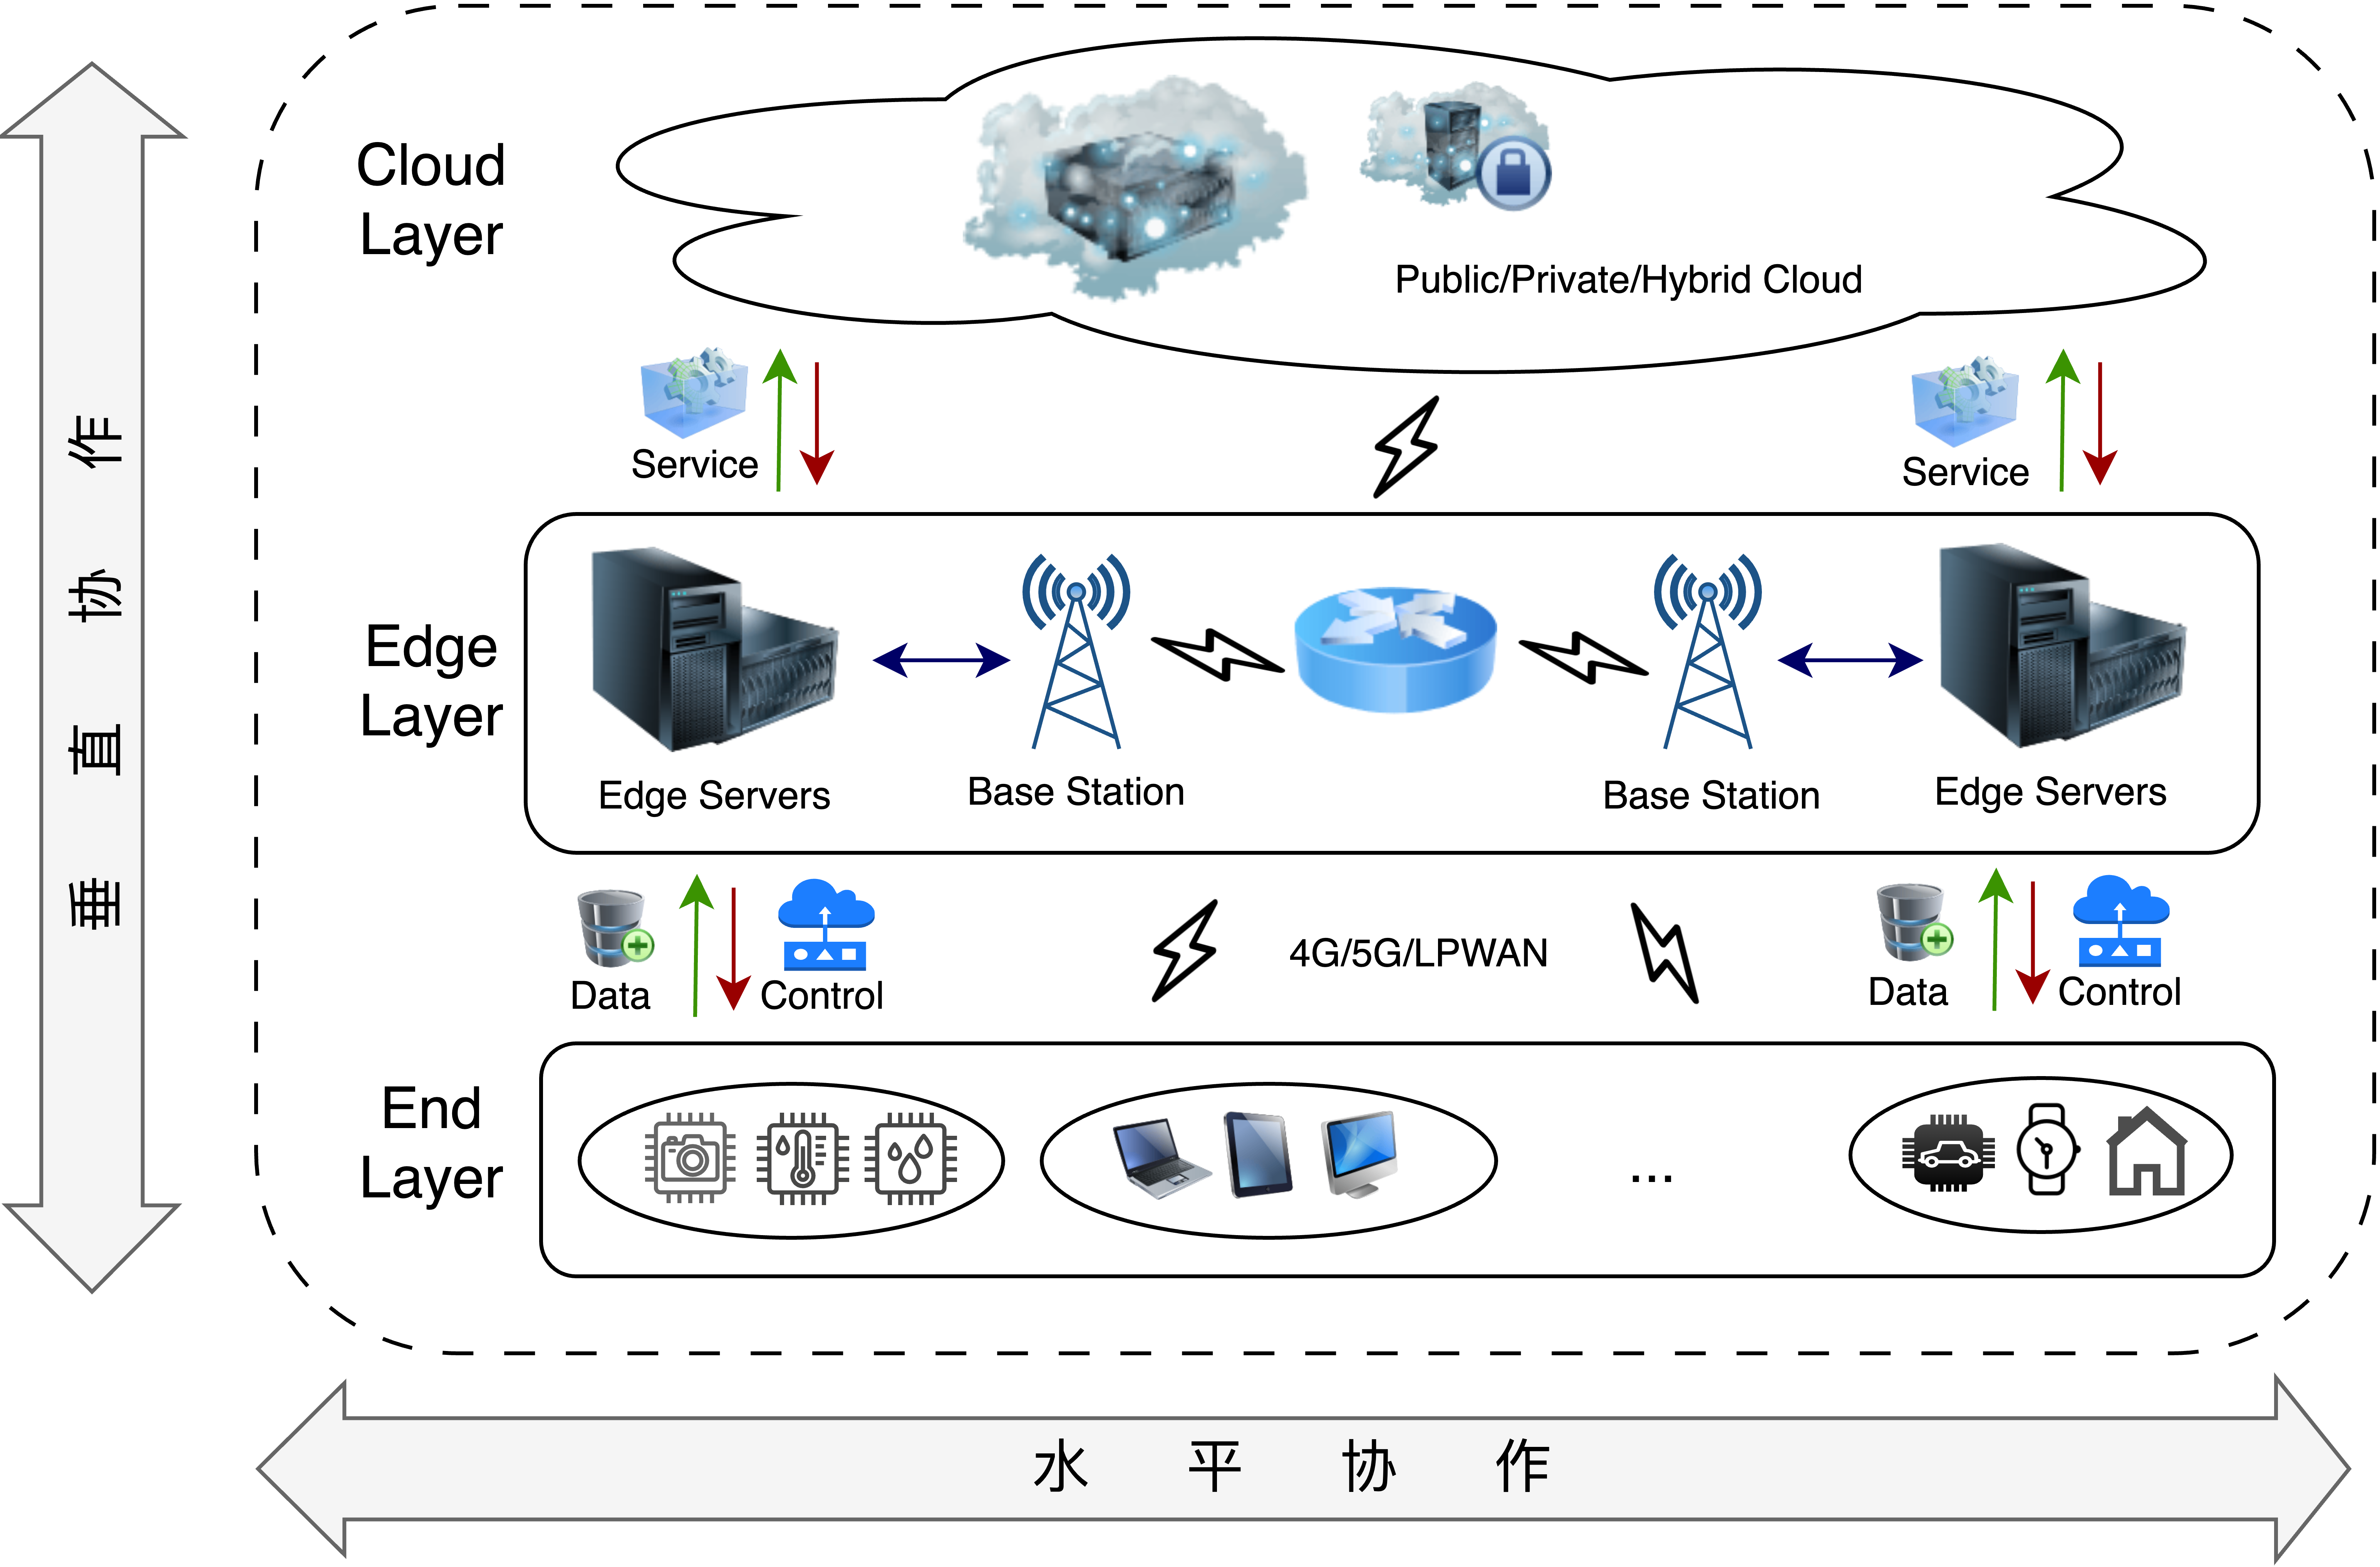
\includegraphics[width=\linewidth]{pics/2-1云边端架构.png}
  \caption{边缘计算架构和异构化的边缘节点}
  \label{fig:my_label}
\end{figure}

Prometheus + Blackbox Exporter 专注于大规模分布式系统的长期监控,通过周期性探测提供延迟和可用性等性能数据,同时支持多种协议的探测和丰富的数据分析功能,但其配置复杂且在实时性要求较高的场景中可能存在一定延迟。


任务分类和模型评估:
图像识别(IMAGE_RECOGNITION, type=1):

大部分图像分类模型(如 ResNet 系列、VGG、EfficientNet 等)通常提供 Top-1 和 Top-5 准确率。
目标检测(OBJECT_DETECTION, type=2):

目标检测模型如 YOLO系列、Faster R-CNN、RetinaNet、SSD 等,通常没有提供 Top-1 或 Top-5 准确率,而是用 mAP(Mean Average Precision)或者 IoU(Intersection over Union)来评估。
语义分割(SEMANTIC_SEGMENTATION, type=3):

语义分割模型如 U-Net、DeepLabV3 等,一般提供 IoU 或 mIoU(Mean Intersection over Union)指标,而不是 Top-1 或 Top-5 准确率。
实例分割(INSTANCE_SEGMENTATION, type=4):

实例分割模型如 Mask R-CNN、YOLACT 等,也通常使用 mAP 或 AP(Average Precision)等评估指标,而不是 Top-1 或 Top-5 准确率。
文本识别(TEXT_RECOGNITION, type=5):

文本识别模型(如 CRNN、Tesseract OCR)一般提供的是 字符准确率(Character Accuracy)或者 Word Error Rate(WER),而不是 Top-1 或 Top-5 准确率。
人脸检测(FACE_DETECTION, type=6):

人脸检测模型如 MTCNN、RetinaFace、FaceNet 等,提供的是 检测准确率,通常以 mAP 或 精确度(Precision)、召回率(Recall)来衡量,而不是 Top-1 或 Top-5 准确率。
图像生成(IMAGE_GENERATION, type=7):

图像生成模型如 GAN、StyleGAN2、DALL·E 等,通常使用 FID(Fréchet Inception Distance) 或 Inception Score 等评估指标,而不是 Top-1 或 Top-5 准确率。



这些 FLOPS(每秒浮点运算次数)是基于模型的架构特点、文献和实际实现中的常见估算得出的,以下是参考的依据和方法:

1. 分类模型 (Type 1)
这些模型的 FLOPS 依据是标准输入尺寸(通常为 224x224)进行的推算:

ResNet 系列:ResNet 的 FLOPS 是公开的,并与层数成比例增加。例如:
ResNet18: 1.8 GFLOPs(官方文档)
ResNet50: 3.8 GFLOPs
ResNet101: 7.6 GFLOPs
ResNet152: 11.3 GFLOPs
VGG 系列:VGG 是一个较早的深度学习模型,因全连接层较多 FLOPS 较高:
VGG16: 15.3 GFLOPs
VGG19: 19.6 GFLOPs
EfficientNet:极其高效,FLOPS 较低:
EfficientNetB0: 0.39 GFLOPs
InceptionV3:约 5.7 GFLOPs,文献明确说明。
DenseNet121:约 2.9 GFLOPs(模型紧凑性导致 FLOPS 较低)。
2. 目标检测模型 (Type 2)
目标检测的 FLOPS 通常远高于分类模型:

YOLO 系列:
YOLOv3: 65.9 GFLOPs(官方文献提供)。
YOLOv4: 72.2 GFLOPs(增强特征提取模块)。
YOLOv5 和 YOLOv7:基于实现的优化,FLOPS 分别为 25.6 和 17.4 GFLOPs。
Faster R-CNN:两阶段检测器,计算密集,约 180 GFLOPs。
RetinaNet:单阶段检测器,FLOPS 为 210。
SSD:约 36 GFLOPs(由于其简化的网络结构)。
3. 语义分割模型 (Type 3)
语义分割模型 FLOPS 依据输入尺寸(512x512)计算:

FCN:约 15 GFLOPs(深度较浅的卷积网络)。
U-Net:更复杂的分割模型,约 27 GFLOPs。
DeepLabV3:由于引入多尺度特征提取,约 24 GFLOPs。
SegNet:受其复杂性,约 30 GFLOPs。
4. 实例分割模型 (Type 4)
实例分割的 FLOPS 高于语义分割:

Mask R-CNN:两阶段检测结合分割任务,约 275 GFLOPs。
YOLACT:轻量级实例分割,约 138 GFLOPs。
Panoptic FPN:处理分割与检测,约 320 GFLOPs。
5. OCR (Type 5)
OCR 模型 FLOPS 较低,输入尺寸常为文本图像:

CRNN:序列预测模型,约 10 GFLOPs。
Tesseract OCR:轻量化 OCR 模型,约 0.5 GFLOPs。
ASTER:较复杂的模型,约 15 GFLOPs。
6. 人脸检测与识别 (Type 6)
输入图像常较小(112x112 或更小):

MTCNN:轻量级网络,约 0.4 GFLOPs。
RetinaFace:更高精度模型,约 1 GFLOPs。
FaceNet:复杂度稍高,约 1.6 GFLOPs。
7. 生成模型 (Type 7)
生成模型 FLOPS 通常根据生成目标的分辨率:

GAN:较基础的生成模型,约 20 GFLOPs。
StyleGAN2:生成高分辨率图像,约 35 GFLOPs。
VQ-VAE-2:复杂生成模型,约 40 GFLOPs。
数据来源:
模型官方文档与论文。
实际 FLOPS 测试(如通过工具 FLOP-counting library 测试)。
深度学习社区的公开资源(如 PyTorch、TensorFlow 实现)。
如果需要更具体的来源或公式,我可以进一步查找相关数据!


验证了KEAS平台在真实边缘环境中的性能优势。实验基于KubeEdge构建双集群管控平面,测试结果显示平台端到端延迟降低39.2\%,服务中断时间减少98\%,在资源利用率、适应性和稳定性方面均优于现有方案,证实了所提云边协同优化方法的有效性。


\item \( C \)表示云层节点集合,\( C = \{ c_1, c_2, \ldots, c_n \} \),每个云层节点 \( c_i \in C \) 配备高性能计算资源(如CPU、GPU、内存),适用于处理计算密集型和数据量大的 AI 任务,例如深度学习模型训练或大规模推理。
    \item \( E \)表示边缘节点集合,\( E = \{ e_1, e_2, \ldots, e_m \} \),每个边缘端节点 \( e_j \in E \) 部署在靠近用户的位置,资源(CPU、内存)有限,适用于低延迟、轻量级的任务,例如实时数据简单处理或轻量级模型推理。
    \item \( D \)表示设备模型集合,\( D = \{ d_1, d_2, \ldots, d_p \} \),每个设备模型 \( d_k \in D \) 是设备的核心定义,设备可以在设备模型的基础上具体实现,包括数据产生的频率、每次产生的数据大小等。
    \item \( A \)表示AI 负载原型集合,\( A = \{ a_1, a_2, \ldots, a_q \} \) ,每个 AI 负载原型 \( a_l \in A \) 包含 AI 的准确率、FLOPS、版本号、处理的事务类型等数据。在不同类型节点上运行的时延可能不一样。
    \item \( N \)表示网络拓扑,是云层和边缘端节点之间的网络连接及其带宽容量。网络拓扑影响数据传输延迟和任务调度决策。


\subsubsection{优化目标}

该模型的调度目标是实现云端和边端节点之间的协同执行,优化以下目标:

\begin{enumerate}
    \item \textbf{最大化成功响应的批处理请求数量} \\
    \[
    f_N(X) = \sum_{r_t \in R} I(\text{request } r_t \text{ is satisfied})
    \]
    其中,\( I \) 为指示函数,表示请求 \( r_t \) 在时延和资源约束下是否成功响应。

    \item \textbf{最小化资源消耗} \\
    \[
    f_C(X) = \sum_{r_t \in R} \sum_{a_l \in A} \sum_{n \in C \cup E} x_{tln} \cdot c_{tln}
    \]
    其中,\( x_{tln} \) 表示请求 \( r_t \) 分配给负载 \( a_l \) 在节点 \( n \) 执行的数据处理比例,\( c_{tln} \) 表示相应的资源消耗。
\end{enumerate}

优化问题形式化为:

\[
\max_{X} f_N(X)
\]
\[
\min_{X} f_C(X)
\]
\[
\text{subject to: 时延、资源容量约束}
\]


KESLang




\subsection*{1. 节点定义}

\subsubsection*{1.1 云端节点}
设云端节点集合为 \( C = \{c_1, c_2, \dots, c_m\} \)。每个云端节点 \( c_i \) 定义如下:
\begin{itemize}
    \item \(\text{CPU}(c_i)\):云端节点 \( c_i \) 的 CPU 容量。
    \item \(\text{MEM}(c_i)\):云端节点 \( c_i \) 的内存容量。
    \item \(\text{GPU}(c_i)\):云端节点 \( c_i \) 的 GPU 容量。
    \item \(\text{BW}(c_i)\):云端节点 \( c_i \) 的带宽容量(单位:数据大小/时间)。
\end{itemize}

\subsubsection*{1.2 边端节点}
设边端节点集合为 \( E = \{e_1, e_2, \dots, e_n\} \)。每个边端节点 \( e_j \) 定义如下:
\begin{itemize}
    \item \(\text{CPU}(e_j)\):边端节点 \( e_j \) 的 CPU 容量。
    \item \(\text{MEM}(e_j)\):边端节点 \( e_j \) 的内存容量。
    \item \(\text{BW}(e_j)\):边端节点 \( e_j \) 的带宽容量。
    \item \(\text{GPU}(e_j) = 0\):边端节点没有 GPU 资源。
\end{itemize}

\subsection*{2. 用户请求定义}
设用户请求集合为 \( R = \{r_1, r_2, \dots, r_k\} \)。每个用户请求 \( r_i \) 定义如下:
\begin{itemize}
    \item \(\text{ID}(r_i)\):请求的唯一标识符。
    \item \(\text{Type}(r_i)\):请求的类型,表示需要处理的 AI 任务类型。
    \item \(\text{Duration}(r_i)\):请求的运行周期时长(单位:时间)。
    \item \(\text{DataCount}(r_i)\):请求包含的数据数量。
    \item \(\text{DataSize}(r_i)\):请求的数据总大小(单位:数据大小)。
    \item \(\text{Accuracy}(r_i)\):请求要求的最低准确率。
    \item \(\text{Source}(r_i)\):请求的节点来源(可以是某个边端节点 \( e_j \))。
\end{itemize}

\subsection*{3. AI 负载定义}
设 AI 负载集合为 \( A = \{a_1, a_2, \dots, a_p\} \)。每个 AI 负载 \( a_i \) 定义如下:
\begin{itemize}
    \item \(\text{ID}(a_i)\):AI 负载的唯一标识符。
    \item \(\text{Name}(a_i)\):AI 负载的名称。
    \item \(\text{SupportedTypes}(a_i)\):能够响应的请求类型集合。
    \item \(\text{Latency\_GPU}(a_i, y)\):在 GPU 环境下,节点 \( y \) 上运行该负载的单次推理时延(单位:时间)。
    \item \(\text{Latency\_NoGPU}(a_i, y)\):在非 GPU 环境下,节点 \( y \) 上运行该负载的单次推理时延(单位:时间)。
    \item \(\text{Throughput}(a_i)\):单次推理的吞吐量(每次推理能处理的图片数量)。
    \item \(\text{Resources}(a_i) = (\text{CPU}(a_i), \text{MEM}(a_i), \text{GPU}(a_i))\):运行所需的资源量。
\end{itemize}

\subsection*{4. 调度目标与约束}

\subsubsection*{4.1 调度决策变量}
定义调度变量:
\begin{itemize}
    \item \( x_{ij} \geq 0 \):表示请求 \( r_i \) 中由 AI 负载 \( a_j \) 处理的数据比例(\(0 \leq x_{ij} \leq 1\),所有负载的比例之和为 1)。
    \item \( y_{ij} \in C \cup E \):表示请求 \( r_i \) 中分配给 AI 负载 \( a_j \) 的任务被分配到的节点(云端节点或边端节点)。
\end{itemize}

约束:
\begin{itemize}
    \item 数据分配总量约束:请求 \( r_i \) 中,分配给所有 AI 负载的数据比例之和等于 1,即:
    \[
    \sum_{j} x_{ij} = 1, \quad \forall r_i \in R
    \]
    其中,\( x_{ij} \) 表示负载 \( a_j \) 处理的比例。
\end{itemize}

\subsubsection*{4.2 约束条件}

\paragraph*{1. 运行时长约束}


\paragraph*{1. 运行时长约束}

请求 \( r_i \) 在运行周期内必须完成其所有数据的处理,约束如下:

\[
\sum_{j} \left( \frac{x_{ij} \cdot \text{DataCount}(r_i)}{\text{Throughput}(a_j)} \cdot \text{Latency}(a_j, y_{ij}) \right) + \frac{\text{DataSize}(r_i)}{\text{BW}(y_{ij})} \leq \text{Duration}(r_i), \quad \forall r_i \in R
\]

其中:
\begin{itemize}
    \item \( x_{ij} \cdot \text{DataCount}(r_i) \):表示负载 \( a_j \) 处理的具体数据量。
    \item \( \text{Throughput}(a_j) \):AI 负载 \( a_j \) 的单次推理吞吐量。
    \item \( \text{Latency}(a_j, y_{ij}) \):AI 负载 \( a_j \) 在节点 \( y_{ij} \) 上的单次推理时延。
    \item \( \frac{\text{DataSize}(r_i)}{\text{BW}(y_{ij})} \):数据传输时延,取决于请求的数据大小和节点 \( y_{ij} \) 的带宽。
    \item \( \text{Duration}(r_i) \):请求的运行周期时长。
    \item \[
            \text{Latency}(a_j, y_i) =
            \begin{cases} 
            \text{Latency\_GPU}(a_j), & \text{if } \text{GPU}(y_i) > 0 \\
            \text{Latency\_NoGPU}(a_j), & \text{if } \text{GPU}(y_i) = 0
            \end{cases}
        \]
\end{itemize}

该约束确保所有分配给负载的任务在请求时长内能够完成。

\paragraph*{2. 准确率约束}

请求的处理结果需满足其准确率要求,考虑数据分配比例后,约束如下:
\[
\sum_{j} x_{ij} \cdot \text{Accuracy}(a_j) \geq \text{Accuracy}(r_i), \quad \forall r_i \in R
\]
其中:
\begin{itemize}
    \item \( x_{ij} \cdot \text{Accuracy}(a_j) \):表示负载 \( a_j \) 处理的比例对应的贡献准确率。
    \item \(\text{Accuracy}(r_i)\):请求 \( r_i \) 对整体任务的最低准确率要求。
\end{itemize}

\paragraph*{3. 资源容量约束}
每个节点的资源总使用量不能超过其可用容量:
\[
\sum_{r_i \in R} x_{ij} \times \text{Resources}(a_j) \leq \text{AvailableResources}(y_i), \quad \forall y_i \in C \cup E
\]

\subsubsection*{4.3 优化目标}

优化目标分为两级优先级:

\paragraph*{1. 一级优化目标:最大化成功响应的请求数量}

目标是优先最大化成功响应的请求数量。定义一个二进制变量:
\[
z_i = 
\begin{cases} 
1, & \text{如果请求 } r_i \text{ 被成功响应(满足所有约束)} \\
0, & \text{否则}
\end{cases}
\]
一级优化目标为:
\[
\max \sum_{r_i \in R} z_i
\]

\paragraph*{2. 二级优化目标:在满足一级目标的基础上最小化带宽利用}

在一级目标下,进一步最小化所有请求的数据传输所消耗的带宽:
\[
\min \sum_{r_i \in R} \sum_{j} \frac{x_{ij} \cdot \text{DataSize}(r_i)}{\text{BW}(y_{ij})}
\]
其中:
\begin{itemize}
    \item \( x_{ij} \cdot \text{DataSize}(r_i) \):表示负载 \( a_j \) 处理的任务对应的数据大小。
    \item \( \text{BW}(y_{ij}) \):节点 \( y_{ij} \) 的带宽。
\end{itemize}

经典的云边协同框架主要面向通用计算任务,通过服务编排机制为容器化负载提供跨云边环境的部署能力。

在运行时管理维度,尚未建立覆盖模型加载、推理执行到效果评估的全生命周期监控体系,特别是工业场景中应对数据漂移的在线学习与模型迭代机制仍不完善。

\paragraph{定义3.2 (终端设备)} 设备$d_i \in \mathcal{D}$定义为:
\[
d_i = (\Lambda_i,\, g_i)
\]
其中:
\begin{itemize}
    \item $\Lambda_i$ 表示静态属性集合,静态属性集$\Lambda_i = \{\rho^{(1)}_i, ..., \rho^{(q)}_i\}$(q的上标在之前是不是使用过,请你修改不要重复)由设备类型$t_i \in \mathcal{T}$约束,存在双射映射$\tau: \mathcal{T} \to \mathcal{H}$使$\tau(t_i) = \mathcal{H}_j$确定管理策略。可通过映射函数$\phi: \Lambda_i \to \sigma_i$推导出单次数据量$\sigma_i \in \mathbb{R}^+$(请你把瞬时数据量的映射函数在这里定义)。
    
    \item $g_i(这个定义的时候介绍公式,然后说明时变频率$\nu_i(t)$的概念就行,不要再写一个item介绍$\nu_i(t)$了): \mathbb{R} \to \mathbb{R}^+$ 表示动态数据生成函数,$g_i(t) = \nu_i(t) \cdot \sigma_i$,其中$\nu_i(t): \mathbb{R} \to [0,\, \nu_i^{max}]$表示时刻$t$的瞬时数据产生频率(单位:Hz)。

(后面的这个是你上次给出的修改的定义,你需要把下面的定义融合到前面的内容中)
    \item 动态生成函数$g_i(t) = \nu_i(t) \cdot \phi(\Lambda_i)$,其中:
    \begin{align*}
        \phi: \mathbb{A} & \to \mathbb{R}^+ \\
        \Lambda_i & \mapsto \prod_{k=1}^q \xi(\rho^{(k)}_i) 
    \end{align*}
    这里$\xi(\cdot)$为属性量化函数(如摄像头$\xi(\rho^{\text{res}})=x \times y$像素数)
    
    \item 频率函数$\nu_i(t) \in \mathcal{V}_i$满足Lipschitz连续性:
    \begin{equation}
        |\nu_i(t+\Delta t) - \nu_i(t)| \leq L_\nu \Delta t
    \end{equation}
    其中$L_\nu$为设备物理特性决定的状态变化率上界
\end{itemize}


设备类型注册表$\mathcal{T} = \{t_\alpha\}_{\alpha=1}^\mu$建立设备类型与管理器之间的映射关系,确保每个设备类型$t_\alpha$对应唯一的管理器$h_\alpha \in \mathcal{H}$。设备元数据通过静态属性集合$\Lambda_i$描述,其构成具有显著的类型差异性。以视觉设备为例,其静态属性集$\Lambda_i$包含成像分辨率(resolution)、色彩位深度(bit depth)、压缩算法(compression)、总线标识(bus info)等可量化参数;而温度传感器则包含量程(range)、精度(accuracy)等测量特性。设备管理器通过动态采集策略调控数据生成过程,其瞬时数据量由静态属性映射函数$\phi(\cdot)$和时变频率$\nu_i(t)$共同决定。静态属性集合$\Lambda_i$可以直接计算出单次采集的数据量,例如视觉设备的单帧数据量可通过分辨率与位深度的乘积经压缩率修正得到,结合瞬时频率$\nu_i(t)$,即可计算单位时间内的数据生成量。瞬时频率$\nu_i(t)$表示设备在某一时刻的数据采集速率,受设备硬件特性和动态调控策略的影响。

设备管理器与设备类型一一对应。设备类型由设备类型注册表$\mathcal{T} = \{t_\alpha\}_{\alpha=1}^\mu$,同时建立建立设备类型与管理器之间的映射关系,确保每个设备类型$t_\alpha$对应唯一的管理器$h_\alpha \in \mathcal{H}$。设备类型注册表中主要定义设备静态属性集合$\Lambda_i$。设备静态属性集合$\Lambda_i$描述,其构成具有显著的类型差异性。以视觉设备为例,其静态属性集$\Lambda_i$包含成像分辨率(resolution)、色彩位深度(bit depth)、压缩算法(compression)、总线标识(bus info)等可量化参数;而温度传感器则包含量程(range)、精度(accuracy)等测量特性。除此之外,设备管理器通过动态采集策略调控数据生成过程,动态采集策略主要是配置瞬时频率$\nu_i(t)$,其表示设备在某一时刻的数据采集速率,并且受设备硬件特性和动态调控策略的影响。静态属性集合$\Lambda_i$可以直接计算出单次采集的数据量,例如视觉设备的单帧数据量可通过分辨率与位深度的乘积经压缩率修正得到,结合瞬时频率$\nu_i(t)$,即可计算单位时间内的数据生成量。



\paragraph{定义3.2 (终端设备)} 终端设备$d_i \in \mathcal{D}$定义为:
\[
d_i = (\Lambda_i,\, g_i)
\]
其中:
\begin{itemize}
    \item $\Lambda_i = (\rho^{(l)}_i)_{l=1}^{\eta}$ 表示静态属性集合($\eta \in \mathbb{N}^+$为属性维度),由设备原型$t_\alpha \in \mathcal{T}$ 通过类型约束$\Phi(t_\alpha) = \{\Lambda_i\}$唯一确定。设备原型$t_\alpha$与设备管理器类型$h_\alpha$满足映射关系$\tau(t_\alpha) = h_\alpha \in \mathcal{H}$。通过属性量化函数:
        \begin{align*}
            \phi: \mathcal{P}^\eta & \to \mathbb{R}^+ \\
            (\rho^{(1)}_i, \ldots, \rho^{(\eta)}_i) & \mapsto \prod_{l=1}^{\eta} \psi_l(\rho^{(l)}_i)
        \end{align*}
    计算单次数据量$\sigma_i = \phi(\Lambda_i)$,其中$\psi_l: \mathcal{P} \to \mathbb{R}^+$为预定义的标准化转换函数。
    \item 动态生成函数$g_i: \mathbb{R} \to \mathbb{R}^+$表示实时数据流量:
        \[
        g_i(t) = \nu_i(t) \cdot \sigma_i
        \]
    其中瞬时频率$\nu_i(t) \in [0, \nu_i^{\max}]$满足Lipschitz连续性约束:
        \[
        \exists L_i > 0,\ \forall t_1, t_2 \in \mathbb{R},\ |\nu_i(t_2) - \nu_i(t_1)| \leq L_i |t_2 - t_1|
        \]
    $L_i$表示设备物理特性决定的最大调节速率。
\end{itemize}


你要扮演云边协同和软件工程的专家,同时深谙人类写论文的方式,有严谨的学术性,最后用latex代码给出,不要出现AI常犯的表达重复、逻辑僵化的问题。下面是你需要处理的需求:


请你根据现有的上下文,抽象出一个设备原型的定义,注意设备原型主要包括原有定义的静态属性,还有一个特殊的协议(比如物理接口(如USB 3.0)或无线协议(如Wi-Fi 6)等,请你抽象这个概念),还有一个设备管理器的属性(一个设备管理器对应一个设备原型),注意新的定义不要与之前出现的符号、上下标重复

为了实现终端设备的定义,本文引入设备原型和设备管理器的概念的概念。设备原型是

1. 请你根据现有的上下文,将修改现有终端设备的定义,首先抽象出设备原型和设备管理器的定义,终端设备的定义修改为设备原型和设备管理器这两个部分
2. 设备原型主要包括终端设备原有定义的静态属性$\Lambda_i = (\rho^{(l)}_i)_{l=1}^{\eta}$,新增一个协议(比如物理接口(如USB 3.0)或无线协议(如Wi-Fi 6)等,请你抽象这个概念,给出一个全局不重复的符号),新增一个符号表示单次数据采集的大小(请你抽象这个概念,给出一个全局不重复的符号,介绍这个符号时,说明可以通过预定义的标准化转换函数其中$\psi_l: \mathcal{P} \to \mathbb{R}^+$,通过相关公式计算出,你可以用原来的公式)
3. 设备管理器主要包括终端设备原有定义中的\item 动态生成函数(全部修改称之为预定义采集策略)$g_i: \mathbb{R} \to \mathbb{R}^+$,新增一个时间触发的方式(比如用户点击以后触发等情况,请你抽象这个概念,给出一个全局不重复的符号)

下面是现有的论文的上下文:





这一设计不仅有助于提升云边协同系统中的设备管理效率,还为复杂场景下的动态调度提供了理论基础。在动态数据采集层面,设备管理器通过配置瞬时采样频率 $\nu_i(t)$ 实现数据生成过程的时变控制。该参数表示设备在任意时刻 $t$ 的采样速率,其取值同时受限于硬件物理特性及开发人员定义的采集策略约束。结合静态属性集合 $\Lambda_i$ 与瞬时频率 $\nu_i(t)$,可精确计算单位时间内的数据生成量。例如,对于视觉设备,单位时间内的数据生成量为单帧数据量与瞬时频率的乘积。



为实现标准化管理,本文构建设备原型注册表 $\mathcal{T} = \{t_\alpha\}_{\alpha=1}^\mu$,其中每个设备原型 $t_\alpha$ 对应唯一设备管理器类型 $h_\alpha \in \mathcal{H}$,形成双射映射$\tau:\mathcal{T}\to\mathcal{H}$。



\paragraph{定义3.2 (设备原型)} 设备原型$t_\alpha \in \mathcal{T}$可表示为一个 3 元组:
\[
t_\alpha = (\Lambda_\alpha,\, \Pi_\alpha,\, \sigma_\alpha)
\]
其中:
\begin{itemize}
    \item $\Lambda_\alpha = (\rho^{(l)}_\alpha)_{l=1}^{\eta}$ 表示静态属性集合($\eta \in \mathbb{N}^+$为属性维度),表征设备的物理特性。
    \item $\Pi_\alpha \in \mathbb{Z}^+$表示通信协议标识符,通过映射表$\chi: \mathbb{Z}^+ \to \mathcal{P}$对应具体协议实现(USB 3.0、Wi-Fi 6等)。
    \item $\sigma_\alpha \in \mathbb{R}^+$表示单次数据采集量,通过标准化转换函数计算:
        \[
        \sigma_\alpha = \phi(\Lambda_\alpha) = \prod_{l=1}^{\eta} \psi_l(\rho^{(l)}_\alpha)
        \]
        其中$\psi_l: \mathcal{P} \to \mathbb{R}^+$为预定义的属性量化函数。
\end{itemize}

\paragraph{定义3.3 (设备管理器)} 设备管理器$h_\alpha \in \mathcal{H}$可表示为一个 2 元组:
\[
h_\alpha = (\nu_\alpha,\, \Theta_\alpha)
\]
其中:
\begin{itemize}
    \item $\nu_\alpha(t) \in [0, \nu_\alpha^{\max}]$ 表示采集策略函数,需满足Lipschitz连续条件:
        \[
        \exists L_\alpha > 0,\ \forall t_1, t_2 \in \mathbb{R},\ |\nu_\alpha(t_2) - \nu_\alpha(t_1)| \leq L_\alpha |t_2 - t_1|
        \]
        $L_\alpha$表示设备物理特性决定的最大调节速率。        
    \item $\Theta_\alpha = \{(\epsilon_k, \kappa_k)\}_{k=1}^m$ 为事件驱动触发器集合,每个触发器包含事件类型$\epsilon_k \in \mathbb{X}$($\mathbb{X}$为预定义事件枚举集)和触发条件$\kappa_k: \mathbb{R}^+ \to \{0,1\}$(当$\kappa_k(t)=1$时激活数据采集)。
\end{itemize}



(表示一种AI负载实例对应一类设备,一类设备可能可以用多种AI负载实例处理,请你按照我的意思写一句话过渡,)

给出AI负载\{\ell_s\}的定义,$\mathcal{L} = \{\ell_s\}_{s=1}^u$ 表示AI负载实例集合,
AI负载实例包括AI框架(给出一个新的符号定义,与前面出现过的符号和上下标不要冲突),硬件架构需求(再给出一个新的符号定义,与前面出现过的符号和上下标不要冲突),最少需要的资源数量(再给出一个符号定义,与前面出现过的符号和上下标不要冲突,包括CPU、GPU等资源,你可以抽象一下,只给出一个资源列表,说明要满足这些需求即可),运算量(flops,你可以查找资料,给出一个更学术的表达),批处理大小(再给出一个新的符号定义,与前面出现过的符号和上下标不要冲突)

(然后写一段话说明云边节点的异构性,云端节点可能有不同的资源,引出节点的定义)

然后给出节点的定义(给出一个新的符号,与前面出现过的符号和上下标不要冲突),节点集合包含$\mathcal{E} = \{e_j\}_{j=1}^m$ 表示边缘节点集合和$\mathcal{C} = \{c_q\}_{q=1}^r$ 表示云端节点集合。节点有如下属性:资源数量(与前面的AI资源需求类似,只是这边的是节点上物理所拥有的资源,用于初步判断AI负载实例能不能部署到相关节点上运行,再给出一个新的符号定义,与前面出现过的符号和上下标不要冲突),硬件架构标签(再给出一个新的符号定义,与前面出现过的符号和上下标不要冲突)。

然后说明可以用一个函数(给出一个新的符号,与前面出现过的符号和上下标不要冲突),参数是AI负载和相关AI负载实例,输出是单次运行的时间,扩写这句话


云边协同AI推理调度模型的运行时行为刻画了实际云边环境下设备流数据调度过程,




\begin{algorithm}
\caption{SWORD: 随机权重优化调度策略}
\label{alg:sword}
\begin{algorithmic}[1]
\REQUIRE 调度上下文$context$,目标函数集合$objectives$,样本数量$N$
\ENSURE 最优部署方案$result$

\STATE \textbf{阶段1:收集部署选项}
\STATE $options \leftarrow \text{CollectDeploymentOptions}(context)$
\IF{$options = \emptyset$}
    \STATE $fallback \leftarrow \text{CreateFallbackOption}(context)$
    \IF{$fallback \neq \null$}
        \STATE \textbf{return} $\text{CreateResult}(fallback)$
    \ELSE
        \STATE \textbf{return} $\text{FailureResult}()$
    \ENDIF
\ENDIF

\STATE \textbf{阶段2:生成随机权重样本}
\STATE $solutions \leftarrow \emptyset$
\FOR{$i=1$ \TO $N$}
    \STATE \text{生成归一化随机权重}
    \STATE $weights \leftarrow \text{RandomWeights}(objectives)$
    
    \STATE \text{评估所有选项}
    \FORALL{$opt \in options$}
        \STATE $\text{ComputeObjectiveValues}(opt, objectives, context)$
        \STATE $score \leftarrow \sum_{obj\in objectives}weights[obj] \times obj.evaluate(opt)$
        \STATE $opt.setScore(score)$
    \ENDFOR
    
    \STATE $\text{SortByScore}(options)$ \COMMENT{按得分降序排序}
    \STATE $bestOpt \leftarrow options[0]$
    \STATE $solutions.add(bestOpt)$
\ENDFOR

\STATE \textbf{阶段3:帕累托前沿分析}
\STATE $paretoFront \leftarrow \emptyset$
\FORALL{$candidate \in solutions$}
    \IF{$\nexists other \in solutions \text{ 使得 } other \prec candidate$}
        \STATE $paretoFront.add(candidate)$
    \ENDIF
\ENDFOR

\STATE \textbf{阶段4:最终方案选择}
\IF{$paretoFront \neq \emptyset$}
    \STATE $finalOpt \leftarrow \arg\max_{opt \in paretoFront}(opt.score)$
\ELSE
    \STATE $finalOpt \leftarrow \arg\max_{opt \in solutions}(opt.score)$
\ENDIF

\STATE \textbf{return} $\text{CreateResult}(finalOpt)$
\end{algorithmic}
\end{algorithm}

\begin{equation}
score(opt) = \sum_{i=1}^{k} w_i \cdot f_i(opt)
\end{equation}
\begin{equation}
w_i \sim U(0,1),\ \sum w_i = 1
\end{equation}
\begin{equation}
a \prec b \iff \forall i\ f_i(a) \geq f_i(b) \wedge \exists j\ f_j(a) > f_j(b)
\end{equation}

方法

SWORD: Stochastic Weighted Optimization for Resource Distribution with Pareto-dominance

"Stochastic" refers to the random sampling of weights used in the algorithm
"Weighted Optimization" captures the core mechanism of using weights for multi-objective functions
"Resource Distribution" describes the algorithm's purpose
"Pareto-dominance" highlights the sophisticated mathematical technique used for final selection

输入:全局集群队列大小,需要调度的数据流,需要生成随机权重的数量
输出:分流比例
首先随机生成权重
然后遍历每一个权重模仿上面的集群内部动态调度算法,实现贪心的方式找到部署结果
对于所有的结果比较生成帕累托前沿。
确定所有的结果

伪代码控制在30行左右

你可以模仿本地动态调度算法的算法,主要就是借鉴上面的格式

首先对于所有的数据流(排序)如有多个,则按照产生数据的大小从大到小排序,优先把数据在本地运行,防止网络开销
然后遍历所有的数据流
    对于所有的数据流按照调度目标计算总时延,把所有的节点按照时延从小到大排序,注意每个节点可能已经有之前的队列了,这边放入的是剩余的容量,将本地设备的数据依次放入本地队列,直到设备数据分配完。

你可以模仿本地动态调度算法的算法,主要就是借鉴上面的格式




(写一段话说明为什么要实现这个调度器编程框架,(请你修改后面的句子,使其更通顺,更具有逻辑,各级调度器的优化目标和约束条件不一样。所以本文设计了调度器编程框架,云边平台各个调度器提供了相关的API可以用于快速的描述优化目标和约束条件))

为了方便各级调度器完成不同的调度目标和约束策略,本文提出了一套编程框架,用于实现之前提出的多目标规划模型和单目标规划等实现

然后说明多目标之间使用min–max normalization的实现多目标的归一化(给出相关的公式)

调度器编程框架

你可以模仿下面的设计写自己的调度器编程框架,要合理同时满足


概述方法内容

在云边协同的环境中,AI推理服务的调度是实现高效、低延迟和高可靠性的核心环节。随着边缘计算和人工智能技术的快速发展,将AI推理能力部署到边缘设备已成为实时决策的关键需求。然而,传统云计算模式在处理实时性要求高的应用时,面临数据传输延迟高和资源集中管理的瓶颈,而边缘计算虽然通过将计算任务下沉到靠近数据源的节点降低了延迟,但受限于边缘设备资源不足,难以独立应对复杂的AI推理任务。为此,云边协同模式通过整合云端的全局调度与边缘的本地化执行,成为优化资源分配和任务执行的有效路径。

(还需修改)


    
    本文设计了一种形式化的云边协同AI推理调度模型,明确定义了模型中的关键组件,如终端设备、AI负载实例、计算节点、计算队列、边缘集群、分层调度框架、运行时状态等,并阐述了数据流驱动的动态调度机制。该模型为后续的调度策略设计提供了理论基础。

(Kubernetes Edge AI Scheduling)



云边协同AI推理平台是在云原生框架KubeEdge基础上构建的系统,旨在通过资源调度实现高效AI模型推理服务。该平台基于第三章中介绍的调度算法,构建了垂直和水平方向的协同机制。系统设计了

\begin{figure}[ht]
  \centering
  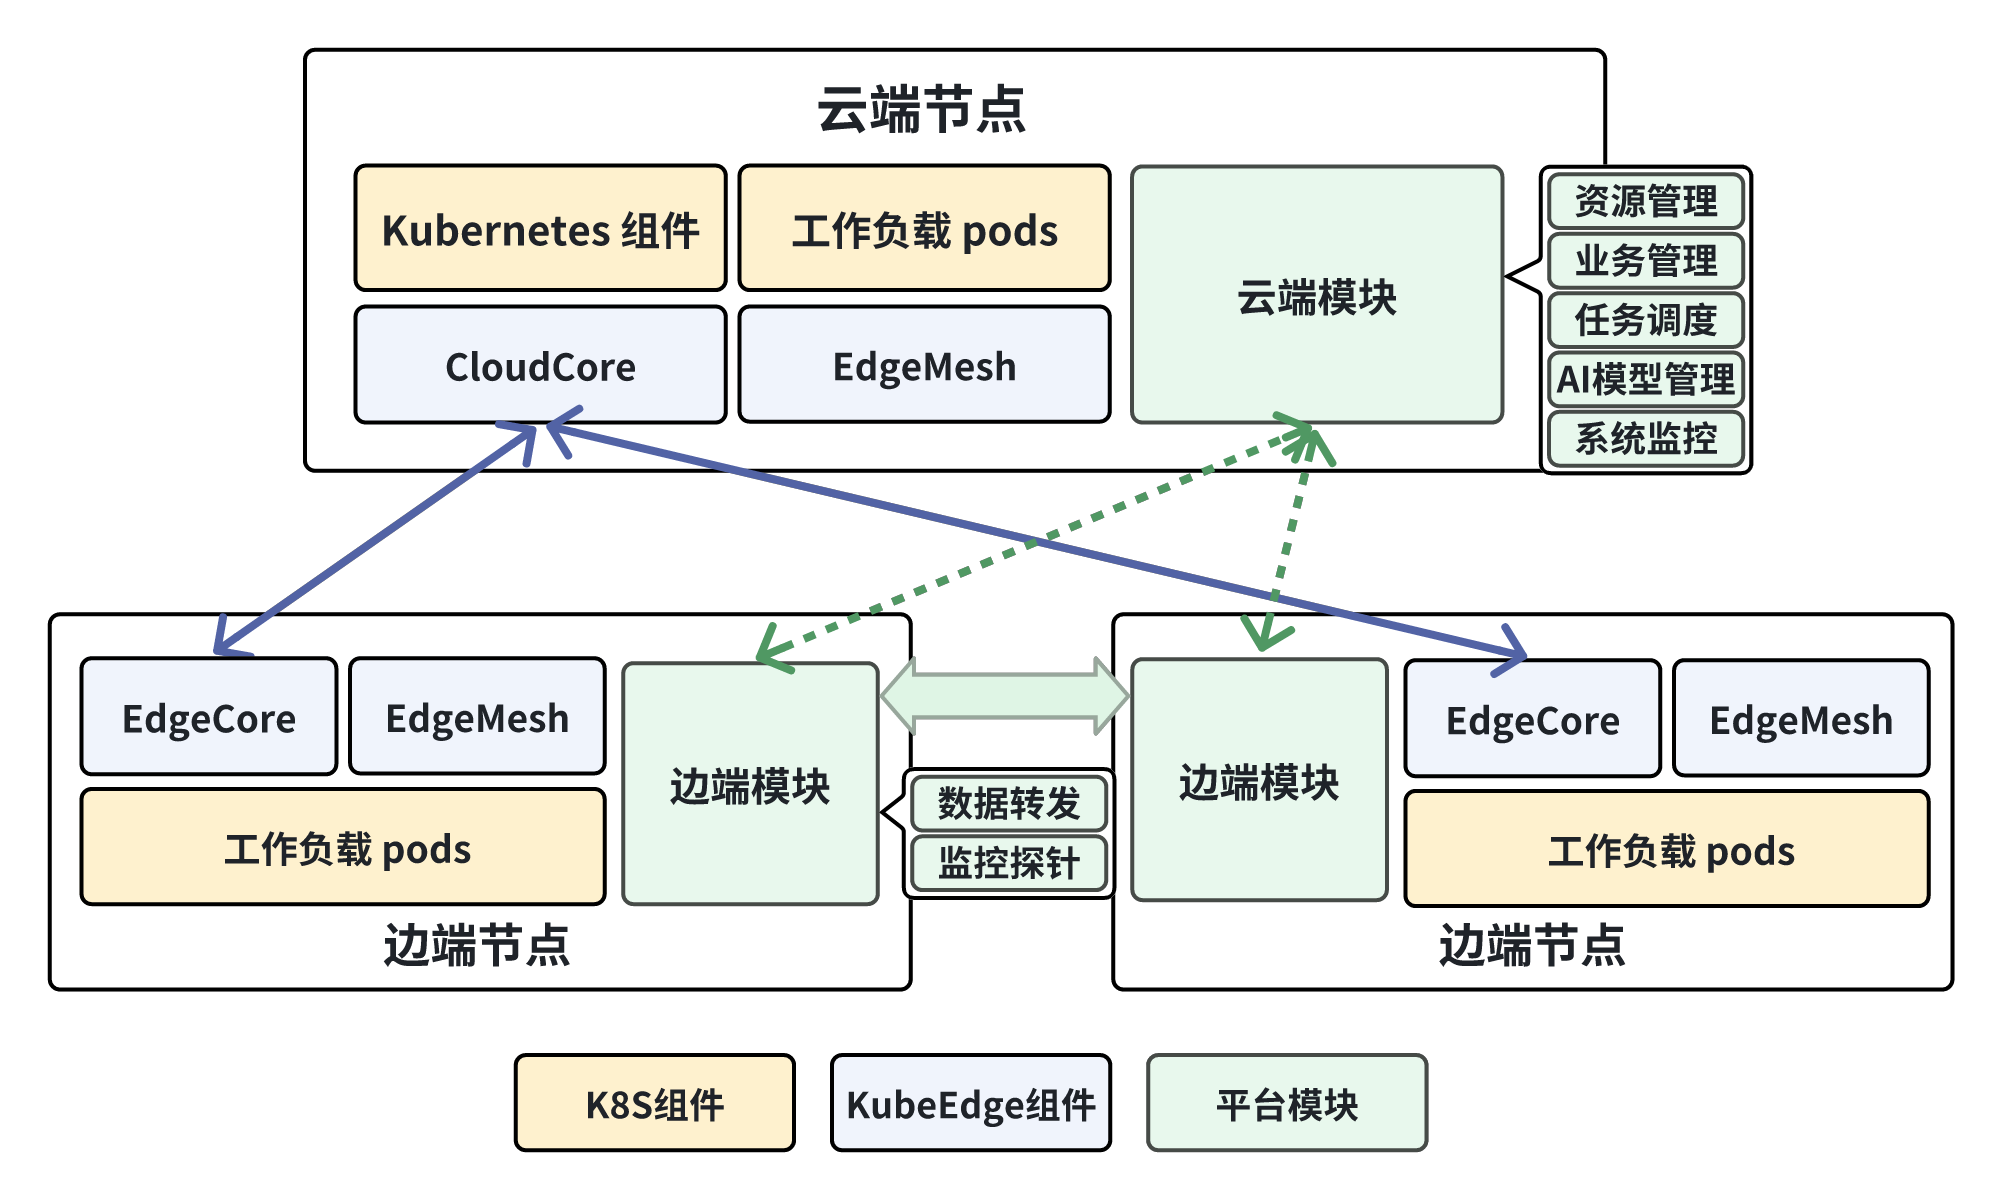
\includegraphics[width=\linewidth]{pics/4-1模块化.png}
  \caption{云边协同AI推理平台总体概览}
  \label{fig:4-1modules}
\end{figure}

为了实现分布式的调度,本文在kubeedge上映射了akka集群,通过akka特有的流处理模式和分布式调度模式actor实现调度模式实现调度,其中实现了三个特有的actor,分别对应云端调度器、边缘调度器和AI推理服务的执行者。

平台的用户主要包括算法工程师、软件开发人员和系统管理员。算法工程师可以通过平台的 AI 模型管理功能,专注于 AI 模型的开发与优化;软件开发人员则可利用数据业务处理服务,专注于数据处理逻辑的实现;系统管理员则通过统一控制台完成节点注册、设备配置及状态监控等运维操作。该平台通过抽象化底层基础设施,使得各角色用户无需关注集群管理细节,显著提升开发部署效率。此外,平台集成实时监控告警系统,并采用基于角色的访问控制的权限隔离,为运维人员提供全链路可观测性,同时确保多租户环境下的系统安全稳定运行。

基于AKKA设计




是运行实际的任务负载。本文中AI模型负载运行由单独的模块负责,通过容器的形式部署在节点上,工作单元只需负责与AI模型相关的预处理、请求转发以及后处理操作(修改前面两句话,使其更通顺,更具有逻辑)。这些任务的具体实现往往因应用场景的不同而存在较大差异,因此系统设计了一个高度灵活的抽象接口。如图\ref{fig:4-6worker}所示,本文定义了一个工作单元的抽象类(WorkerActor),并进一步抽象出工作负载(Workload)和任务结果(WorkResult)。通过继承 WorkerActor 类,用户可以根据具体需求扩展其实现,从而满足不同业务场景下的定制化需求。

此外,工作单元还承担了运行时状态监测的功能。它实时采集任务运行的关键指标,包括订阅的设备数据主题的消息频率、AI 模型处理单次推理的时间等。这些数据不仅用于监控节点的运行状况,还为调度系统的决策提供了重要依据。

同时,工作单元监测任务的运行状态,包括订阅的mqtt topic(用中文)数据的频率,AI负载处理一次数据的时间等,用于运行时监测节点的运行情况。

在工作单元的运行过程中,其创建由边缘调度器(Manager)负责管理。具体而言,当需要创建一个新的工作单元时,系统首先会在本地环境中查找是否存在对应的工作负载类文件。如果本地不存在,则会从云端的远程仓库(如 Maven 或自定义的 Mioio 仓库)动态下载对应的 JAR 包,并通过类加载机制将所需的类注入到运行时环境中。这一过程利用了 Spring 框架的动态类加载能力,确保了工作单元能够根据需求动态扩展和实例化,从而显著提升了系统的灵活性和适应性。

第三层是工作单元(Worker),其核心功能包括订阅 MQTT 协议的流式数据、执行推理任务负载,以及实现数据分流等操作,工作单元的功能会在具体在后面的数据路由服务详细介绍(修改这一段的表达)。


为了进一步分析AI负载实例在动态环境中的性能表现,本文将系统运行时间划分为等长时间窗$\{t_\omega\}_{\omega=1}^\infty$,其中$t_\omega = [\tau_\omega, \tau_\omega + \Delta t)$表示第$\omega$个调度时间窗,$\Delta t$为时间窗长度参数。

如何在保证服务质量(QoS)的前提下,动态调整模型在云端和边缘节点之间的部署位置,以适应实时变化的应用场景?


与此同时,数据隐私和安全性问题日益突出,集中式处理模式因高昂的加解密成本及潜在泄露风险,在敏感场景下的适用性受到挑战\cite{soveizi2023security}。

,并通过本地化处理加强了隐私保护

然而,当前云边协同方案在高效调度方面仍存在不足:K3s 缺乏专门的云边协同组件,而 KubeEdge 和 OpenYurt 尽管引入了更精细的节点分组与管理功能,但其调度算法仍沿用传统云端任务分配逻辑,难以完全满足云边协同场景对低延迟和高可靠性的要求,尤其在部署位置优化上存在改进空间。为此,本研究综合评估后选定 KubeEdge 作为底层架构,原因在于:首先,KubeEdge 从设计上原生支持云边协同,将“云-边-端”融为一体,提供丰富的边缘设备管理和数据处理能力,相较于缺乏云边协同组件的 K3s,它更适合大规模、多功能的边缘计算场景,同时相比 OpenYurt,它对边缘端资源要求更低且设备管理更优;其次,作为 CNCF 项目,KubeEdge 拥有活跃的社区支持以及成熟的文档、示例和教程,为开发与运维提供了坚实保障。


这些方案依托 Kubernetes 的容器编排与管理能力,通过功能裁剪适应边缘场景的资源约束,有的扩展了一定的边缘自治能力,确保系统在网络不稳定或与云端短暂失联时仍能维持关键服务(判断这句话是否适配上面的三个工具)。这些模块可以通过扩展或加入一些其他的组件用来实现云边协同,但其负载均衡仍沿用传统云端任务分配逻辑,难以完全满足云边协同场景对低延迟和高可靠性的要求。(修改这一部分)

云计算自诞生以来,凭借虚拟化技术和大规模数据中心架构,为各行业提供了弹性且可扩展的资源共享模式。随后,容器化技术和微服务架构的引入催生了云原生概念,进一步提升了云端系统的可移植性与交付效率\cite{deng2024cloud}。在此过程中,Kubernetes\cite{kubernetes} 和 Docker Swarm\cite{dockerswarm} 等编排工具成为云原生生态的核心支柱,实现了大规模集群管理和自动化部署。基于这些先进的云端技术,工业界逐渐将云计算的计算、网络与存储能力延伸至边缘侧,以满足低延迟和高可靠性的应用需求。目前,较为成熟的边缘计算方案包括 Rancher 公司开发的 K3s\cite{fogli2021performance}、华为贡献给云原生基金会(CNCF)的 KubeEdge\cite{xiong2018extend} 以及阿里巴巴开源的 OpenYurt\cite{openyurt2023}。这些方案依托 Kubernetes 的容器编排与管理能力,通过功能裁剪适应边缘场景的资源约束,通过扩展具备一定的边缘自治能力,确保系统在网络不稳定或与云端短暂失联时仍能维持关键服务。其中K3s 缺乏专门的云边协同组件,而 KubeEdge 和 OpenYurt 尽管引入了更精细的节点分组与管理功能,但其负载均衡仍沿用传统云端任务分配逻辑,难以完全满足云边协同场景对低延迟和高可靠性的要求。

(找一找有没有学者在OpenYurt的研究)(修改这两段)

或扩展与分布式需求,并(修改这一段)

然而,当前云边平台在高效资源调度方面仍存在不足:K3s 缺乏专门的云边协同组件,而 KubeEdge 和 OpenYurt 尽管引入了更精细的节点分组与管理功能,但其负载均衡仍沿用传统云端任务分配逻辑,难以完全满足云边协同场景对低延迟和高可靠性的要求。



此外,部分研究人员围绕计算卸载策略展开了深入研究(修改这一句,实现过渡)。然而,这些工作主要针对通用计算负载,可以为云边协同下的AI推理调度提供参考,但是还是没有考虑AI推理中遇到的动态环境感知机制、和模型集成与部署机制的问题。

并没有充分考虑异构节点上AI推理相关的服务质量要求,比如传输的网络带宽

在学术界,研究人员提出了多种

针对云边协同中的资源调度问题,已有大量研究从不同角度提出了创新解决方案。

部分学者在上述云边平台的基础上,优化调度(修改这一段)。





然而,并没有充分考虑深度学习场景下的特殊性。



提高边缘云集群中的集群资源利用率和服务时间方面的服务质量


Lingayya等人\cite{lingayya2024dynamic}提出的动态任务卸载框架在KubeEdge平台上利用区块链技术有效优化了资源分配和隐私保护,可以

然而其多智能体协作强化学习的调度设计更偏向于适应动态变化的任务卸载需求,未从节点协同的角度出发实现。

Mutichiro等人\cite{mutichiro2021qos}在 IoT-Edge 云环境中设计了一种基于服务时间的 QoS 调度器 STaSA ,减少 QoS 违规。




Lingayya等人提出的动态任务卸载框架虽然在KubeEdge平台上通过和区块链技术优化了资源分配和隐私保护,

Lingayya等人提出了基于 KubeEdge 的动态任务卸载框架,结合机器学习优化资源分配和任务卸载,并通过多层区块链机制保护数据隐私。

并没有考虑到真实云边场景下设备流式数据驱动的方式(修改这一句话)。

但是其工作的任务流是确定的,并没有考虑到真实云边场景下设备流式数据驱动的方式。

。



这些方案在资源分配和延迟优化方面展现了潜力,但其调度策略较为单一,难以适应云边协同中多变的网络环境和资源约束。




然而,这些工作主要针对通用计算负载,

仅关注时延优化,未充分考虑深度学习应用中准确率对系统性能的影响。Salem 等人\cite{salem2023toward}提出了推理交付网络(IDN)和 INFIDA 策略,尝试解决深度学习中的延迟与准确性权衡,

但其研究未能充分考虑实时场景变化对模型部署位置的动态调整需求,导致在动态服务质量(QoS)适应性方面表现不佳。例如,当节点异常或故障风险增加时,系统可能需优先降低延迟以避免服务中断,而对准确性的要求可适当放宽。




此外,部分研究人员围绕计算卸载策略展开了深入研究

此外,还有研究人员围绕云边协同下的计算卸载策略展开了深入研究(修改这一句话)。例如,Urgaonkar 等人\cite{urgaonkar2015dynamic}将负载调度建模为马尔可夫决策过程,结合李雅普诺夫优化实现实时调整;
Han 等人\cite{han2019ondisc}提出 OnDisc 算法,通过残余密度优先策略满足延迟敏感需求;Meng等人\cite{meng2019online}设计的 Dedas 算法引入截止期限概念,优化单节点与多节点场景的卸载效率;部分研究\cite{崔玉亚2021一种面向移动边缘计算的多用户细粒度任务卸载调度方法,邝祝芳2022基于深度强化学习的多用户边缘计算任务卸载调度与资源分配算法,郑守建2022一种基于综合匹配度的边缘计算系统任务调度方法,张斐斐2023边缘计算中协作计算卸载与动态任务调度}利用启发式或强化学习方法提升调度性能。然而,这些工作主要针对通用计算负载,处于尚未充分考虑云边协同环境下的AI推理调度,缺乏动态环境感知机制和模型集成与部署机制等问题(修改这一句说明缺陷的语句)。


    
针对传统调度方法缺乏对网络状态和设备负载实时感知的不足,本文设计了自适应动态资源感知调度方法。该方法通过离线阶段构建节点推理性能预测模型生成算力画像,在线阶段融合实时网络状态与设备负载特征,构建多目标优化函数,实现动态资源感知调度。调度框架支持动态添加优化目标与切换优化策略,可灵活应对多样化场景需求,提高了资源分配效率和系统稳定性。

为验证所提出的云边协同AI推理模型和优化方法的有效性,本文实现了KEAS原型系统。该系统基于KubeEdge和Akka,构建了高效分布式AI推理架构,实现了云端控制中心、边缘节点管理器和任务执行器的层次化协作。云端通过K8s Informer机制实时监控集群状态并动态分配任务,边缘侧支持资源弹性扩缩与优先级调度。实验结果表明,KEAS平台在真实边缘环境中的端到端延迟降低了39.2\%,服务中断时间减少了98\%,资源利用率、适应性和稳定性均优于现有方案,充分证明了本文方案的有效性。




\section{KubeEdge及相关技术}

\subsection{KubeEdge的基础架构}

KubeEdge 是由华为主导开发的一款轻量级开源边缘计算平台,旨在解决边缘计算场景中的关键问题,例如边缘节点与云端之间的网络管理,以及边缘节点离线时的会话维护。其架构由云端核心(Cloud Core)和边缘核心(Edge Core)两部分组成,如图 \ref{fig:2-3kubeedge} 所示。云端核心主要负责统一管理分布式的边缘应用服务,而边缘核心则运行在地理上分布的边缘节点中,为物联网应用服务提供支持。

\begin{figure}[ht]
  \centering
  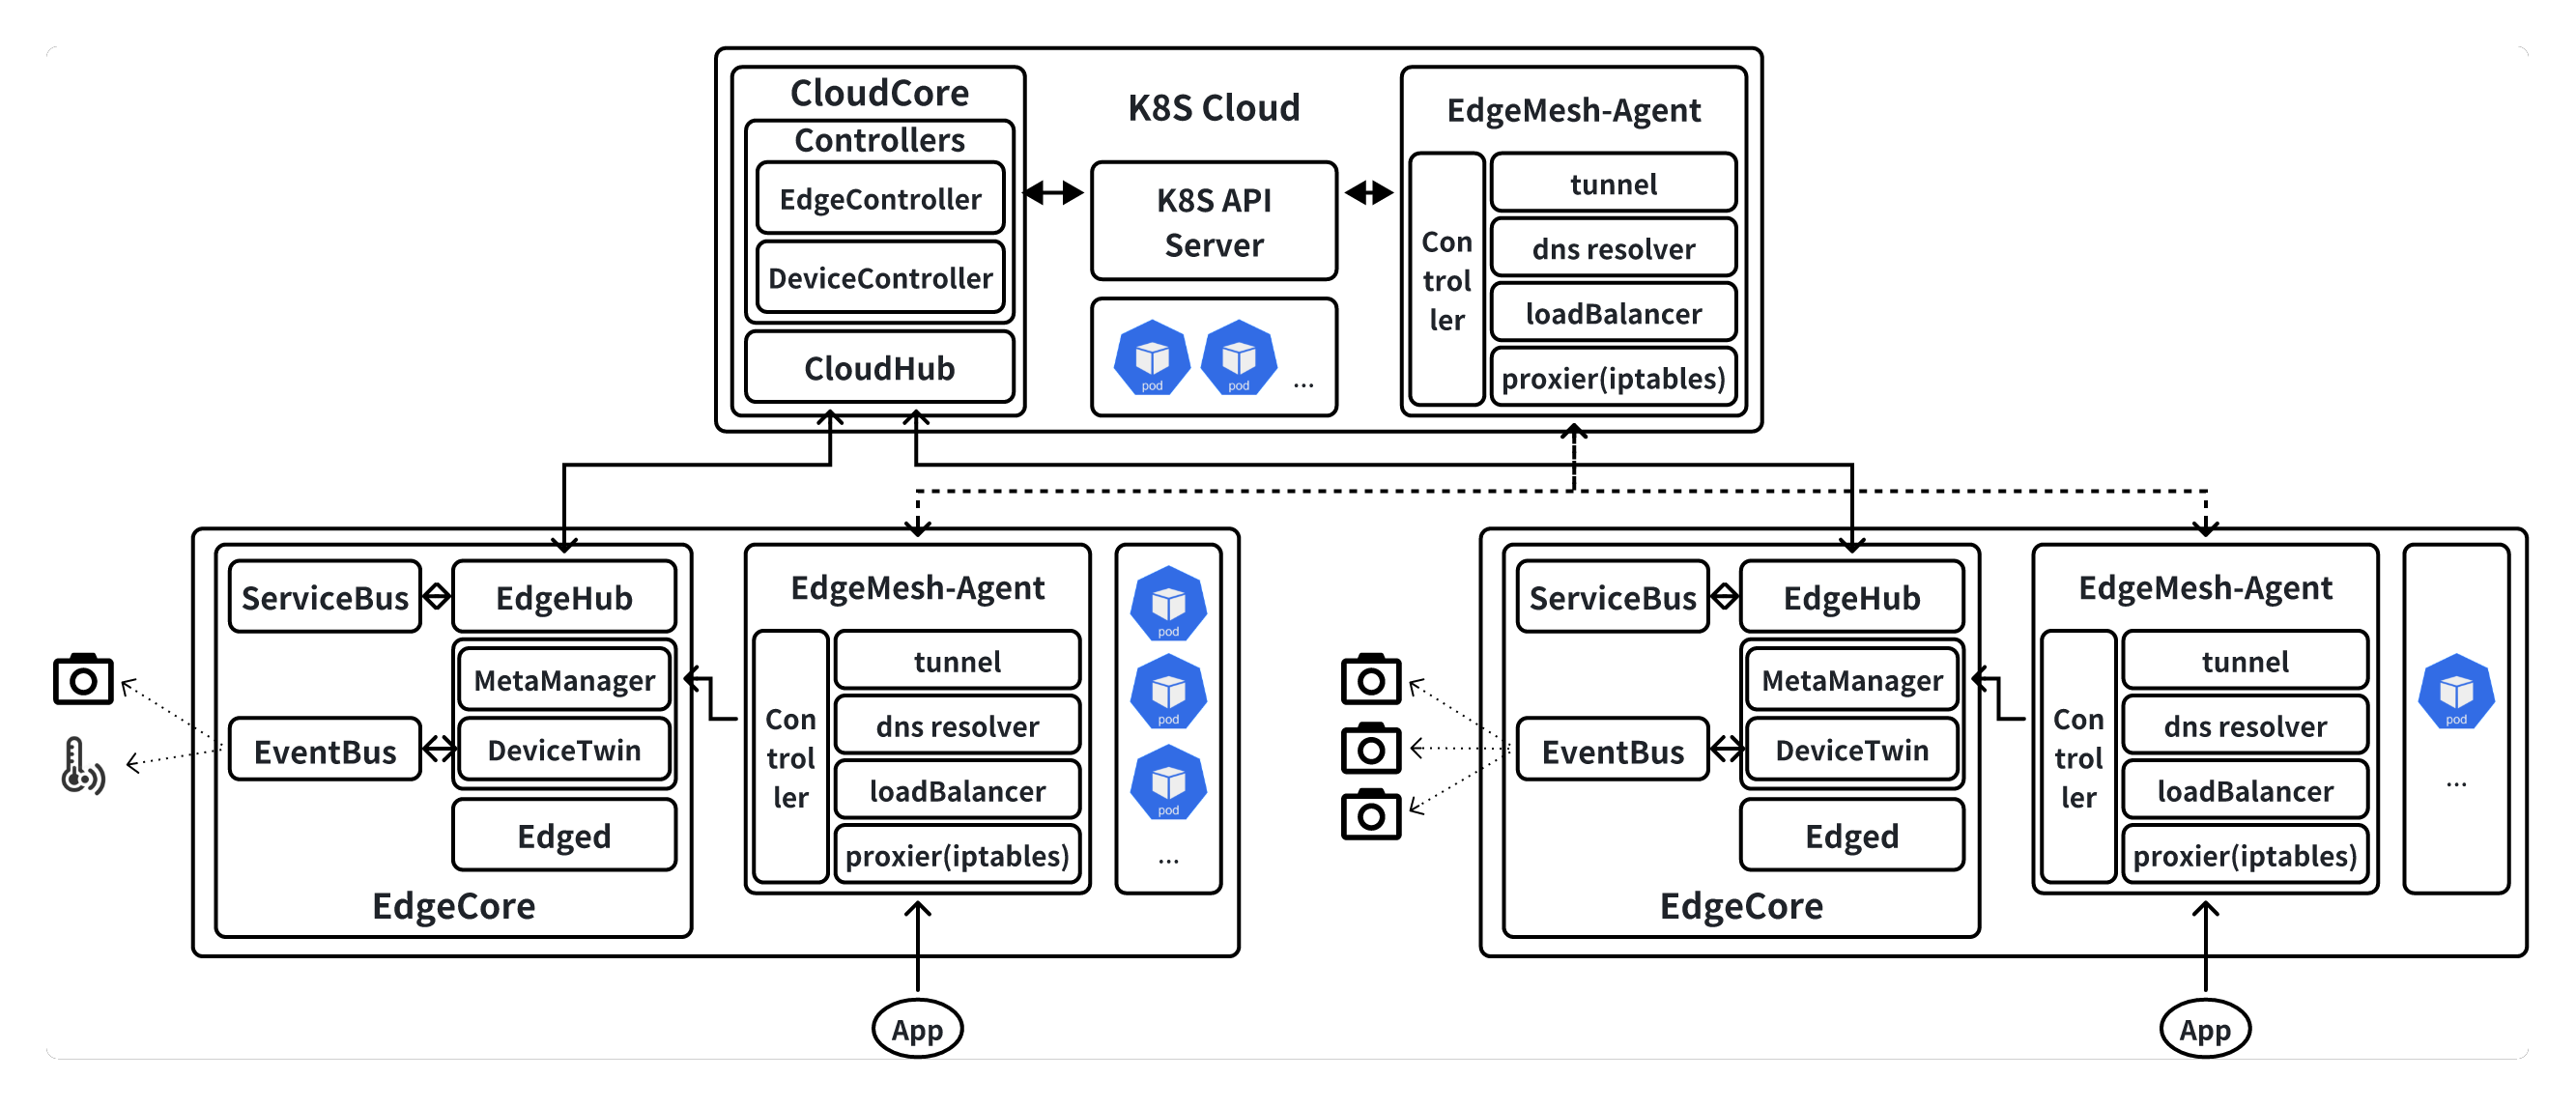
\includegraphics[width=\linewidth]{pics/2-2kubeedge.png}
  \caption{KubeEdge 的基础架构}
  \label{fig:2-3kubeedge}
\end{figure}

云端核心由控制器(Controller)和 CloudHub 两个组件组成,其中控制器分为边缘控制器(Edge Controller)和设备控制器(Device Controller):边缘控制器负责 Kubernetes API Server 和边缘核心之间的事件同步,而设备控制器专注于物联网设备的管理与更新;CloudHub 则作为控制器与边缘核心之间的通信中介,负责监控云端状态变化、缓存消息,并通过 socket 实现双向通信。

边缘核心主要包括以下五个组件:EdgeD 负责运行和管理基于容器的应用,支持 pod 管理、生命周期事件生成、机密管理、容器运行时支持以及工作负载部署;EdgeHub 负责边缘与云端之间的通信,通过 socket 连接实现资源同步、设备状态更新及消息转发;EventBus 提供 MQTT 客户端交互功能,支持发布/订阅机制;DeviceTwin 用于存储设备状态并同步到云端,同时为应用提供查询接口;MetaManager 作为 EdgeD 和 EdgeHub 之间的消息处理器,负责元数据的存储与检索。

\subsection{EdgeMesh的基础架构}

EdgeMesh 是 KubeEdge 集群的数据平面组件,主要提供高可用支持、服务发现和流量代理功能。它利用 LibP2P 技术在边缘节点之间搭建通信网络:对于局域网内的节点,直接访问即可完成数据交互;在跨局域网场景下,则通过打洞隧道技术或中继流量实现数据传输。此外,EdgeMesh 借助 EdgeHub - CloudHub 隧道分发元数据,从而无需直接访问云端,并通过在节点层面部署的 DNS 服务器提升服务搜索的可靠性。在负载均衡方面,EdgeMesh 采用 Istio 的目标规则(DestinationRule),提供轮询和随机等方案,以确保流量在各 Pod 间高效分配,如图 \ref{fig:2-3edgemesh} 所示。

\begin{figure}[ht]
  \centering
  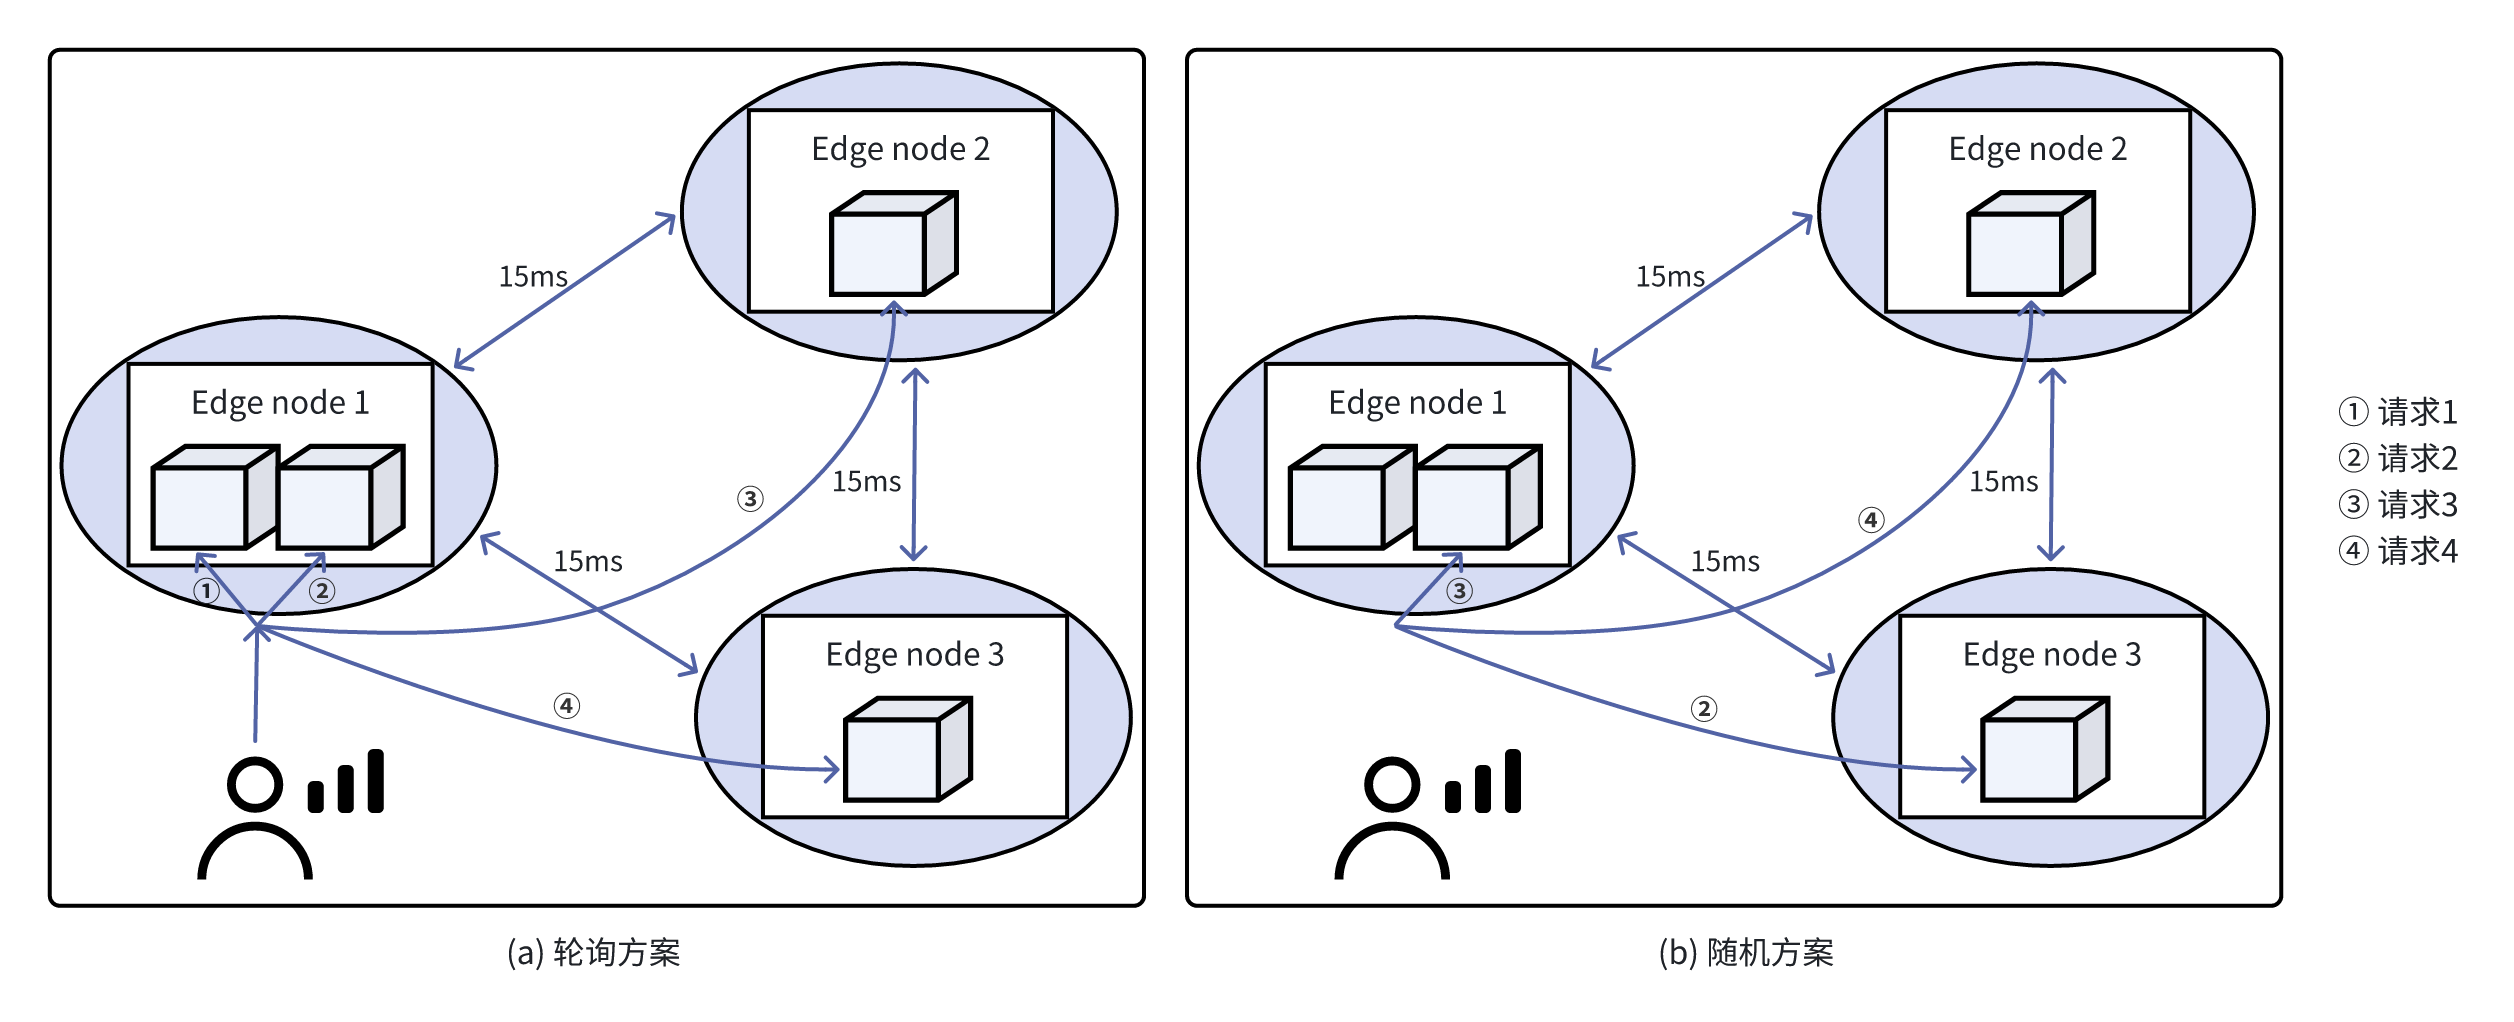
\includegraphics[width=\linewidth]{pics/2-3edgemesh.png}
  \caption{KubeEdge 中的负载均衡方案}
  \label{fig:2-3edgemesh}
\end{figure}

然而,EdgeMesh 并未考虑边缘节点间转发请求所带来的额外延迟。由于边缘计算环境中节点通常地理位置分散,跨节点间的流量转发会显著增加网络时延,降低集群整体吞吐量。针对此问题,Kim 等人\cite{kim2023local}提出了本地调度方案:当边缘节点收到用户请求后,将其平均分配给同一节点上的 Pod,而非转发给远程节点。这样不仅避免了跨节点流量转发导致的高延迟,还能在本地边缘节点即时处理用户请求,从而提升系统的整体吞吐量。然而,本地调度方案也存在不足之处。由于边缘端基础设施通常故障率较高且维护成本较高,当某节点掉线时,部分请求可能无法满足服务质量需求。为解决这些问题,Haja 等人\cite{haja2019sharpening} 提出了 Pod 占位符机制。该机制通过调度算法为每个 Pod 分配一个具有反亲和性(Anti-Affinity)的占位符。当 Pod 所在的主机节点发生故障时,占位符可以迅速在符合延迟约束的其他节点上重新启动 Pod,从而确保服务的连续性。但是,该方法主要关注单节点的可靠性,未能充分利用分布式边缘节点之间的协同能力,限制了系统在高负载场景下的扩展性和整体可靠性。



边缘节点具有异构性,这些节点可能配备低功耗的 CPU、高并行处理能力的多核 GPU,或专用的 AI 加速器(如 VPU)等硬件资源。这种硬件异构性导致节点在计算能力、存储容量和能耗限制上存在显著差异,从而显著增加了资源分配与利用优化的复杂性。在边缘端评估AI推理性能时,推理时延是一个至关重要的指标。针对异构边缘设备的监测需求,最直接的方法是在目标设备上实际运行模型并测量推理时延。这种硬件和网络特性的异构性导致节点在计算能力、存储容量和能耗限制上存在显著差异,从而显著增加了资源分配与利用优化的复杂性。为了提高效率,部分学者\cite{he2018amc,tan2019mnasnet}提出了基于浮点运算次数(FLOPs)的方法。这种方法通过计算模型的FLOPs来快速估算推理时延,无需实际部署模型,适用于初步的模型筛选阶段。然而,FLOPs并不能完全反映硬件的执行特性,如内存带宽限制,也无法考虑运行时的优化技术,如算子融合等。因此,基于FLOPs的预测结果与实际时延之间往往存在显著偏差,适合精度要求不高的场景。Zhang 等人\cite{zhang2021nn} 提出了 nn-Meter 工具,旨在更准确地预测不同边缘设备上的模型推理时延。nn-Meter通过设计一系列测试用例,自动检测模型在特定设备上的推理执行单元(即内核),并识别出设备上的算子融合规则。基于这些信息,nn-Meter能够递归地将整个模型划分为多个内核,从而更精确地捕获设备上的实际执行行为,显著提高了时延预测的准确性。nn-Meter 的核心技术包括以下几个方面,如图 \ref{fig:2-5nnmeter} 所示:首先,根据模型设计和硬件延迟特性对内核配置进行剪枝;其次,通过迭代采样过程自动选择最优配置进行检测,而非采用随机选择策略;最后,利用机器学习回归器学习采样数据的非线性关系,构建高效的内核级延迟预测器。(修改这一段,使得其简洁,富有逻辑)



\section{边缘端节点监测技术}

边缘端通常由多种类型的节点组成,包括硬件配置各异的设备和具有不同网络带宽与延迟特性的连接\cite{cooke2020model,varghese2021survey,barbalace2020edge}。例如,这些节点可能配备低功耗的 CPU、高并行处理能力的多核 GPU,或专用的 AI 加速器(如 VPU)等硬件资源。

\subsection{节点推理能力监测技术}

在边缘端评估AI推理性能时,推理时延是一个至关重要的指标。针对异构边缘设备的监测需求,最直接的方法是在目标设备上实际运行模型并测量推理时延。这种方法能够提供最真实可靠的数据,但需要为每个设备和模型组合逐一部署和测试。当面对多样化的边缘设备和大规模的候选模型时,这种方法的时间成本极高,难以满足快速迭代和开发的需求。

为了提高效率,部分学者\cite{he2018amc,tan2019mnasnet}提出了基于浮点运算次数(FLOPs)的方法。这种方法通过计算模型的FLOPs来快速估算推理时延,无需实际部署模型,适用于初步的模型筛选阶段。然而,FLOPs并不能完全反映硬件的执行特性,如内存带宽限制,也无法考虑运行时的优化技术,如算子融合等。因此,基于FLOPs的预测结果与实际时延之间往往存在显著偏差,适合精度要求不高的场景。而在准确性与效率之间寻求平衡的方案中,Zhang 等人\cite{zhang2021nn} 提出了 nn-Meter 工具,旨在更准确地预测不同边缘设备上的模型推理时延。nn-Meter通过设计一系列测试用例,自动检测模型在特定设备上的推理执行单元(即内核),并识别出设备上的算子融合规则。基于这些信息,nn-Meter能够递归地将整个模型划分为多个内核,从而更精确地捕获设备上的实际执行行为,显著提高了时延预测的准确性。nn-Meter 的核心技术包括以下几个方面,如图 \ref{fig:2-5nnmeter} 所示:首先,根据模型设计和硬件延迟特性对内核配置进行剪枝;其次,通过迭代采样过程自动选择最优配置进行检测,而非采用随机选择策略;最后,利用机器学习回归器学习采样数据的非线性关系,构建高效的内核级延迟预测器。

\begin{figure}[ht]
  \centering
  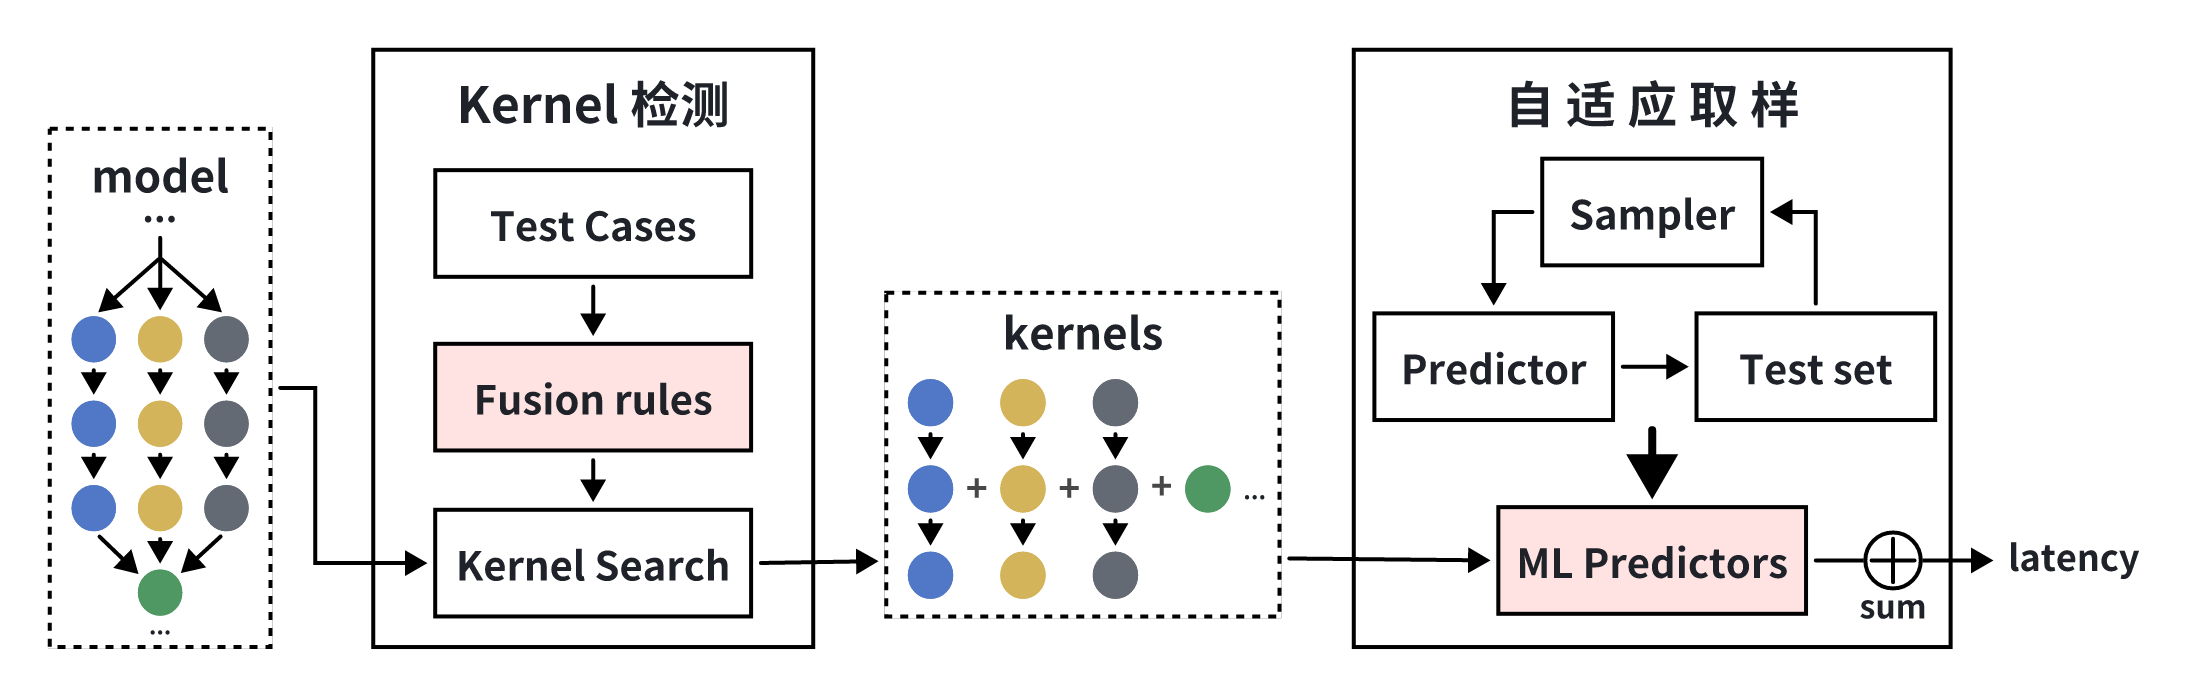
\includegraphics[width=\linewidth]{pics/2-5nnmeter.png}
  \caption{nn-Meter工具的架构}
  \label{fig:2-5nnmeter}
\end{figure}

节点批处理的监测

\subsection{通信监测技术}


然而,Kubernetes 的调度逻辑主要针对云端高性能节点设计,在边缘环境中存在适配性不足的问题,面临资源协调与应用协作管理的双重挑战。在资源协调方面,云边网络具有松散耦合的结构和较高的通信时延,导致云端调度器难以及时掌握边缘资源的实时利用率,从而无法在最佳时机完成任务的优化调度。在应用协作方面,现有云端调度机制对用户服务质量的感知和支持不足,难以有效应对云边协同应用中任务的垂直卸载和水平迁移需求,这进一步增加了应用协作管理的复杂性。

但是说明AI模型运行的过程中的某些框架可能会出现

为了解决上述问题,Lingayya 等人\cite{lingayya2024dynamic} 提出了一种创新的资源管理与任务调度方案,旨在提高边缘计算环境的适应性和运行效率。该方案在边缘节点部署高效的监测模块,实时采集设备资源状态(包括计算能力、内存使用、网络带宽等)和任务队列信息,同时利用多智能体协同强化学习方法,通过多个智能体在共享环境中协作,综合各自的目标和能力,优化整体系统性能。此外,Shan 等人\cite{shan2024kces} 提出了一种资源分配算法。当资源评估结果显示当前节点无法满足任务需求时,该算法通过动态调整任务的资源分配方案,使节点能够容纳更多任务,同时确保任务的最小资源需求,从而最大化资源利用率。如果调整后资源仍无法满足需求,则通过任务水平迁移,将任务分配到其他边缘节点。此外,该方案结合设备的监控模式,对任务进行合理卸载,选择合适的边缘节点或云节点执行,从而实现云边协同的垂直卸载。


近年来,随着深度学习技术的广泛应用,AI推理在各种场景中的需求迅速增长。深度学习模型通过大规模数据训练完成特征提取和参数优化后,在推理阶段能够快速生成预测结果。尽管训练阶段因计算密集和高I/O需求而备受关注,但推理任务的重要性随着实时性要求和边缘设备数据的激增而日益凸显。长期以来,推理被认为较训练更为简单,因其无需复杂的迭代优化。然而,海量传感设备和低延迟需求使得推理任务对系统性能和资源分配提出了新的挑战。在此背景下,云边协同计算通过整合云端的高计算能力和边缘端的低延迟特性,成为解决AI推理问题的重要范式。

云边协同计算旨在通过任务分配和资源优化,结合云端和边缘端的各自优势,以满足AI推理的多样化需求。目前,AI推理服务主要通过两种方式实现:一是边缘设备运行轻量化模型以提供实时响应;二是云端通过“机器学习即服务”(MLaaS)平台支持复杂模型的高吞吐量推理。然而,这两种方式均存在局限性。边缘设备受限于计算能力和存储空间,难以支持高精度的大型模型,而云端服务则因网络延迟难以满足严格的实时性要求。云边协同通过智能资源编排,在性能与延迟之间寻求平衡。例如,轻量任务可分配至边缘端以降低延迟,而复杂计算则交由云端处理,从而提升整体系统效率。这一方法为AI推理提供了一种兼顾灵活性与性能的解决方案。



针对边缘端资源限制问题,研究者提出了模型拆分技术,通过将深度学习模型分解并分布到多个计算单元上,以提升推理效率。Lane等人\cite{lane2016deepx} 提出的DeepX框架通过运行时层压缩(RLC)和深度架构分解(DAD)优化移动设备的推理性能。RLC利用奇异值分解(SVD)压缩模型权重,减少计算量和内存需求,并通过估计器控制压缩程度以维持准确性;DAD则将模型分解为多个单元块,分配至本地和远程处理器,最大化资源利用率。此外,Teerapittayanon等人\cite{teerapittayanon2017distributed} 提出的分布式深度神经网络(DDNN)架构将训练好的模型映射到云、边缘和本地设备上,通过分布式计算缓解通信成本和资源限制问题。这些方法在推理过程中重组各单元块的计算结果,确保输出预测的完整性。然而,模型拆分技术与本文研究的模型调度方法在云边协同中具有互补性,两者各自解决不同层面的问题,为未来进一步结合两种技术提供了可能性。这种结合可以为边缘计算场景下的深度学习推理服务提供更高效、更灵活的解决方案。



在分布式环境中,Actor 模型通过其独特的设计有效避免了传统并发模型中的资源争用问题。每个 Actor 拥有独立的状态,并且其状态仅能通过接收到的消息进行更新,这种机制确保了 Actor 之间不会相互干扰,从而消除了竞态条件的发生。为了应对复杂的任务负载,Actor 模型引入了动态任务分配机制:当某个 Actor 接收到任务时,它可以通过 \texttt{spawn} 操作在网络中动态创建新的 Actor 实例,从而实现工作负载的分而治之。例如,在物联网(IoT)应用程序中,传入的任务通常被划分为多个子任务,并通过 \texttt{spawn} 操作将这些子任务分配给新创建的 Actor 进行并发处理。这种方式不仅显著加快了任务执行速度,还缩短了系统的响应时间。此外,每个 Actor 在任务处理过程中会持续监控网络中其他 Actor 的状态,以便及时检测错误并传播相关信息,从而增强了系统的容错能力,并实现了对分布式环境中错误的快速定位与处理。基于 Actor 模型的编程语言如 Erlang 和 Scala 在这一领域发挥了重要作用。Erlang 由 Armstrong 开发,旨在支持高可用性分布式系统的构建 \cite{armstrong2007history},而 Scala 则通过 Akka 框架提供了对 Actor 的原生支持,兼具函数式编程与面向对象编程(OOP)的特性,并运行于 Java 虚拟机(JVM)之上。近年来,随着云计算和边缘计算(Fog Computing)的兴起,Actor 编程模型在分布式系统中的应用得到了进一步推动,尤其是在边缘计算环境中,可扩展性和容错性成为处理和分析 IoT 应用程序的关键特性 \cite{srirama2021akka}。


\paragraph{定义3.9 (分层调度框架)} 分层调度框架$\mathcal{S}$可表示为一个 3 元组
\[
\mathcal{S} = (S_L, S_B, S_C)
\]
其中:
\begin{itemize}
    \item $S_L$表示本地调度器,负责在计算节点内部对终端设备的流处理任务进行局部调度与资源分配。
    \item $S_B$表示边缘集群调度器,用于在边缘计算集群范围内对终端设备的流处理任务进行协调性调度和优化。
    \item $S_C$表示云端全局调度器,旨在实现跨边缘与云端的全局范围内终端设备流处理任务的统一调度与资源管理。
\end{itemize}

上述分层调度框架中的每个调度器均具有独立的优化策略,这些策略在不同层级上分别关注局部资源利用率、集群范围内的负载均衡以及全局资源的最优分配。为了系统化描述各层级调度器的策略选择机制,并实现从终端设备到边缘集群再到云端的全链路协同优化,本文引入了统一的调度优化策略形式化定义。

\paragraph{定义3.10 (调度优化策略)} 调度优化策略$\mathcal{S}_{\text{opt}}(\mathcal{V}_G^κ)$可表示为一个 2 元组
\[
\mathcal{S}_{\text{opt}}(\mathcal{V}_G^κ) = (\Upsilon_{t_\omega}^κ, \Lambda_{\text{QoS}})
\]

其中:
\begin{itemize}
    \item $\Upsilon_{t_\omega}^κ = (\mathcal{Q}_{t_\omega}^κ, \mathcal{G}_{t_\omega}^κ)$ 表示层次化运行时状态,可以对应节点级、集群级和全局级状态,定义详见定义3.13。
    \item $\Lambda_{\text{QoS}} = (\Psi_{\text{con}}, \Theta_{\text{obj}})$ 表示服务质量指标(QoS),其中$\Psi_{\text{con}} = \{\phi_\eta\}_{\eta=1}^\rho$ 表示调度约束集,每个约束$\phi_\eta$可表示为:
        \[
        \phi_\eta: \mathbb{R}^{|\mathcal{V}_G^\iota|} \to \{0,1\}, \quad \phi_\eta(\mathbf{x}) = 
        \begin{cases}
            1, & \text{满足约束} \\
            0, & \text{违反约束}
        \end{cases}
        \]
    $\Theta_{\text{obj}} = (\theta_\zeta, \omega_\zeta)_{\zeta=1}^\sigma$ 表示多目标优化函数,其中$\theta_\zeta: \mathbb{R}^{|\mathcal{V}_G^\iota|} \to \mathbb{R}$ 为第$\zeta$个目标函数,$\omega_\zeta \in [0,1]$ 为对应权重,满足$\sum_{\zeta=1}^\sigma \omega_\zeta = 1$。
\end{itemize}

为完整描述数据在云边协同架构中的流动路径及其动态特性,本文引入数据流转图的概念。数据流转图不仅能够捕捉数据流在节点间的流动方向,还能反映网络拓扑对数据传输的影响。

\paragraph{定义3.12 (数据流转图)} 数据流转图$\mathcal{G}(\mathcal{V}_{G}^{κ})$可表示为一个参数化的2元组:
\[
\mathcal{G}(\mathcal{V}_{G}^{κ}) = (\mathcal{V}_{G}^{κ}, \mathcal{E}_G)
\]
其中:
\begin{itemize}
    \item $\mathcal{V}_{G}^{κ} \subseteq \mathcal{V}$ 表示当前上下文中的动态节点集合,其元素可以表征不同粒度的计算实体:当$|\mathcal{V}_{G}^{κ}|=1$时表示单个计算节点;当$\mathcal{V}_{G}^{κ} = \mathcal{B}_k$时表征边缘集群$B_k$的节点集合;当$\mathcal{V}_{G}^{κ} = \mathcal{V}$时则覆盖全局计算节点。
    \item $\mathcal{E}_G \subseteq \mathcal{V}_{G}^{κ} \times \mathcal{V}_{G}^{κ}$ 表示数据流传输边集合,每条边$e_{uv} = (v_u, v_v) \in \mathcal{E}_{G}^{κ}$表示数据从节点$v_u$到节点$v_v$的单向传输路径。
\end{itemize}

在数据流转图中,每条数据流传输边不仅描述了数据的传输路径,还隐含了与之相关的传输开销。为了精确量化数据流在云边协同架构中的时空特性,本节重点分析跨层级传输时延模型。在时间窗$t_\omega = [\tau_\omega, \tau_\omega + \Delta t)$内,终端设备 $d_i$ 的数据采集总流量可进一步表示为:

\begin{equation}
G_i^{\tau_\omega} = \varsigma_\beta \cdot g_i^{\tau_\omega}
\end{equation}

其中$\varsigma_\beta$ 表示单次数据采集量(见定义3.2)。

\subsubsection{层次化运行时状态}

在动态调度过程中,系统的运行时状态可分解为计算资源状态与数据流转状态两个正交维度。基于定义3.7的计算队列与定义3.11的数据流转图,本文构建运行时状态的形式化模型:

\paragraph{定义3.13 (层次化运行时状态)} 层次化运行时状态$\Upsilon_{t_\omega}^κ$在时间窗$t_\omega$内可表示为一个 2 元组:
\[
\Upsilon_{t_\omega}^κ = (\mathcal{Q}_{t_\omega}^κ, \mathcal{G}_{t_\omega}^κ)
\]
其中:
\begin{itemize}
    \item $\mathcal{Q}_{t_\omega}^κ = \{\mathcal{Q}_s^j(t_\omega)\}_{s \in \mathcal{L}, j \in \mathcal{V}_G^κ}$表示 $\mathcal{V}_G^κ$ 表示上下文相关的队列状态,其作用域由$\mathcal{V}_G^κ$的粒度决定:
        \[
        \mathcal{Q}_{t_\omega}^κ = 
        \begin{cases}
            \{\mathcal{Q}_s^j\}_{s \in \mathcal{L}}, & |\mathcal{V}_G^κ|=1 \ (\exists v_j \in \mathcal{V}) \\
            \bigcup_{e \in \mathcal{B}_k} \{\mathcal{Q}_s^e\}_{s \in \mathcal{L}}, & \mathcal{V}_G^κ = \mathcal{B}_k \ (B_k \in \mathcal{B}) \\
            \{\mathcal{Q}_s^j\}_{s \in \mathcal{L}, j \in \mathcal{V}}, & \mathcal{V}_G^κ = \mathcal{V}
        \end{cases}
        \]
    \item $\mathcal{G}_{t_\omega}^κ = (\mathcal{V}_G^κ, \mathcal{E}_G(t_\omega))$表示动态数据流转图,具体定义详见定义3.12。
\end{itemize}

基于层次化运行时状态$\Upsilon_{t_\omega}^κ$的形式化建模,三级协同调度架构中的各层级调度器可依据其决策域粒度,动态获取适配的系统状态视图。这种层次化状态感知机制使得各层级调度器既能聚焦其决策域内的核心优化目标,又能通过状态参数传递实现跨层协同,形成局部响应与全局优化的动态耦合。

具体如下:

\begin{itemize}
    \item \textbf{本地设备数据流的处理量最大化}:本地节点应优先处理直连设备的流式数据,优化目标可形式化为:
    \[
    \mathop{\text{maximize}} \sum_{d_i \in \mathcal{D}_{j}} z_{ij}^{t_\omega} \cdot g_i^{t_\omega},
    \]
    \item \textbf{跨节点协作流量最小化}:通过最小化跨节点协作处理的数据流量,减少网络传输开销和系统资源消耗,优化目标可形式化为
    \[
    \mathop{\text{minimize}} \sum_{d_i \in \mathcal{D}_j} (1 - z_{ij}^{t_\omega}) \cdot g_i^{t_\omega} \cdot \varsigma_{i\beta}
    \]
\end{itemize}
为了确保上述优化目标的实现,本地调度策略需满足以下约束条件:

\begin{itemize}
    \item \textbf{计算队列容量约束}:本地与外部数据流的总分配量不得超过节点$v_j$的计算能力极限。具体而言,分配至节点的数据采集量应满足:
    \[
    \sum_{d_i \in \mathcal{D}} z_{ij}^{t_\omega} \cdot g_i^{t_\omega} \leq \Lambda_s^j(t_\omega) \quad \forall \ell_s \in \mathcal{L}_j,
    \]
    其中$\mathcal{D}$表示本地与外部终端设备的并集。
    
    \item \textbf{分流完整性约束}:每个本地设备的数据流需完整分配至计算节点集合,确保数据流不丢失且合理分布。具体而言,分流变量需满足完整性约束:
    \[
    \sum_{v_l \in \mathcal{V}} z_{il}^{t_\omega} = 1 \quad \forall d_i \in \mathcal{D}_j,
    \]
    其中,$\mathcal{V}$表示所有可用计算节点的集合,分流变量 $z_{ij}^{t_\omega}$ 的取值范围需满足 $z_{ij}^{t_\omega} \in [0,1]$。

    \item \textbf{资源适配性约束}:AI 负载实例 $\ell_s$ 需要与节点 $v_j$ 的资源供给和硬件架构相匹配,以确保负载实例能够顺利部署并高效运行。具体而言,需满足以下条件:
    \[
    \rho_j \geq \mathcal{R}_s \quad \text{且} \quad \alpha_j \in \mathcal{A}_s,
    \]
    其中$\rho_j$ 和 $\mathcal{R}_s$ 分别表示节点 $v_j$ 的资源供给向量和负载实例 $\ell_s$ 的资源需求向量;$\alpha_j$ 和 $\mathcal{A}_s$ 分别表示节点 $v_j$ 的硬件架构和负载实例 $\ell_s$ 的硬件架构需求。
\end{itemize}

综上所述,本地调度策略的优化问题可形式化为以下多目标模型:

\[
\begin{aligned}
\mathop{\text{maximize}}\quad & \sum_{d_i \in \mathcal{D}_j} z_{ij}^{t_\omega} \cdot g_i^{t_\omega} \\
\mathop{\text{minimize}}\quad & \sum_{d_i \in \mathcal{D}_j} (1 - z_{ij}^{t_\omega}) \cdot g_i^{t_\omega} \cdot \varsigma_{i\beta} \\
\text{s.t.}\quad 
& \sum_{d_i \in \mathcal{D}} z_{ij}^{t_\omega} \cdot g_i^{t_\omega} \leq \Lambda_s^j(t_\omega) \\
& \sum_{v_l \in \mathcal{V}} z_{il}^{t_\omega} = 1,\ \forall d_i \in \mathcal{D}_j ,\ 0 \leq z_{ij}^{t_\omega} \leq 1\\
& \rho_j \geq \mathcal{R}_s,\ \alpha_j \in \mathcal{A}_s
\end{aligned}
\label{eq:local_scheduling}
\]

\begin{itemize}
    \item \textbf{端到端时延最小化}:总时延由推理时延与传输时延两部分构成。对于设备 $d_i$ 的数据流分配至节点 $e_{kj}$的情形,总时延可分解为:
    \[
    \Theta_{\text{total}} = \underbrace{\Theta_{\text{inf}}(\ell_s, e_{kj})}_{\text{推理时延}} + \underbrace{\Theta_{\text{tran}}(e_{kj'}, e_{kj}, G_{ik}^{t_\omega})}_{\mathclap{\text{集群内传输时延}}}
    \]
    其中,$e_{kj'}$ 为设备的原始本地节点,$G_{ik}^{t_\omega} = g_{i,\text{res}}^{t_\omega} \cdot z_{ikj}^{t_\omega} \cdot \varsigma_\beta$ 表示设备 $d_i$ 分配至节点 $e_{kj}$ 的数据流量。优化目标可形式化为:
    \[
    \mathop{\text{minimize}} \sum_{d_i \in \mathcal{D}} \sum_{e_{kj} \in \mathcal{E}_k \setminus v_j} z_{ikj}^{t_\omega} \cdot \Theta_{\text{total}}
    \]
    即最小化所有设备数据流在集群内部节点间的端到端时延。
    \item \textbf{集群内部设备数据流处理量最大化}:边缘集群应优先处理其集群内部直连设备的数据流,优化目标可形式化为:
    \[
   \mathop{\text{maximize}} \sum_{d_i \in \mathcal{D}_k} \sum_{e_{kj} \in \mathcal{E}_k \setminus v_j} z_{ikj}^{t_\omega},
   \]
   其中 $\mathcal{D}_k$ 表示归属集群 $B_k$ 的终端设备集合。
   \item \textbf{跨域协作流量最小化}:最小化跨域协作处理的数据流量,优化目标可形式化为
    \[
    \mathop{\text{minimize}} \sum_{d_i \in \mathcal{D}_k} \left(1 - \sum_{e_{kj} \in \mathcal{E}_k \setminus v_j} z_{ikj}^{t_\omega}\right) \cdot g_{i,\text{res}} \cdot \varsigma_\beta
    \]
\end{itemize}
为了确保上述优化目标的实现,集群内部调度策略需满足以下约束条件:

\begin{itemize}
    \item \textbf{边缘集群计算队列容量约束}:  
    边缘集群内所有节点的计算队列总容量不得超过其最大吞吐量限制。具体而言,分配至每个节点的数据采集量应满足:
    \[
    \sum_{d_i \in \mathcal{D}} z_{ikj}^{t_\omega} \cdot g_i^{t_\omega} \leq \Lambda_s^{kj}(t_\omega) \quad \forall e_{kj} \in \mathcal{E}_k,
    \]
    其中,$\Lambda_s^{kj}(t_\omega)$ 表示节点 $e_{kj}$ 在时间窗 $t_\omega$ 内对负载实例 $\ell_s$ 的最大吞吐量,$\mathcal{D}$表示全部的终端设备设备。
    
    \item \textbf{边缘集群设备数据流完整性约束}:边缘集群中每个设备的数据流需完整分配至计算节点集合,确保每个设备的数据流被完整分配且不丢失。具体而言,分流变量需满足完整性约束:
    \[
    \sum_{v_l \in \mathcal{V}} z_{l}^{t_\omega} = 1 \quad \forall d_i \in \mathcal{D}_k \quad z_{l}^{t_\omega} \in [0, 1], 
    \]
    其中,$\mathcal{V}$表示所有可用计算节点的集合,$\mathcal{D}_k$ 表示归属集群 $B_k$ 的终端设备集合。
    
    \item \textbf{边缘集群设备资源适配性约束}:AI 负载实例 $\ell_s$ 需要与目标节点 $e_{kj}$ 的资源供给和硬件架构相匹配。具体而言,需满足以下条件:
    \[
    \rho_{kj} \geq \mathcal{R}_s \quad \text{且} \quad \alpha_{kj} \in \mathcal{A}_s \quad \forall e_{kj} \in \mathcal{E}_k ,
    \]
    其中,$\rho_{kj}$ 和 $\mathcal{R}_s$ 分别表示节点 $e_{kj}$ 的资源供给向量和负载实例 $\ell_s$ 的资源需求向量;$\alpha_{kj}$ 和 $\mathcal{A}_s$ 分别表示节点 $e_{kj}$ 的硬件架构和负载实例 $\ell_s$ 的硬件架构需求。
\end{itemize}

综上所述,边缘集群内部调度策略的优化问题可形式化为以下多目标模型:

\[
\begin{aligned}
\mathop{\text{minimize}}\quad & \sum_{d_i \in \mathcal{D}} \sum_{e_{kj} \in \mathcal{E}_k} z_{ikj}^{t_\omega} \cdot \Theta_{\text{total}} \\
\mathop{\text{maximize}}\quad & \sum_{d_i \in \mathcal{D}_{B_k}} \sum_{e_{kj} \in \mathcal{E}_k} z_{ikj}^{t_\omega} \cdot g_i^{t_\omega} \\
\text{s.t.}\quad 
& \sum_{d_i \in \mathcal{D}_{B_k}} z_{ikj}^{t_\omega} \cdot g_i^{t_\omega} \leq \Lambda_s^{kj}(t_\omega), \quad \forall e_{kj} \in \mathcal{E}_k \\
& \sum_{v_{l} \in \mathcal{V}} z_{il}^{t_\omega} = 1, \quad z_{il}^{t_\omega} \in [0,1], \quad \forall d_i \in \mathcal{D}_{B_k} \\
& \rho_{kj} \geq \mathcal{R}_s, \quad \alpha_{kj} \in \mathcal{A}_s, \quad \forall e_{kj} \in \mathcal{E}_k 
\end{aligned}
\label{eq:cluster_scheduling}
\]

\subsubsection{边缘集群调度优化算法}


为了更精确地刻画节点的服务行为并动态跟踪其负载状态,本文引入计算队列的概念,用于表征节点 $v_j$ 在时间窗 $t_\omega$ 内为 AI 负载实例 $\ell_s$ 维护的服务请求列表及其容量限制。

\paragraph{定义3.7 (计算队列)} 计算队列$\mathcal{Q}_s^j(t_\omega)$可表示为一个 2 元组::
\[
\mathcal{Q}_s^j(t_\omega) = \left( \Lambda_s^j(t_\omega),\, \lambda_s^j(t_\omega) \right)
\]
其中:
\begin{itemize}
    \item $\Lambda_s^j(t_\omega) \in \mathbb{Z}^+$表示AI负载实例$\ell_s$在节点$v_j$于时间窗$t_\omega$内的最大吞吐量,可用公式$Q(\ell_s, v_j, t_\omega)$计算。
    \item $\lambda_s^j(t_\omega) \in \mathbb{N}$ 表示当前队列长度,需满足容量约束 $0 \leq \lambda_s^j(t_\omega) \leq \Lambda_s^j(t_\omega)$。
\end{itemize}

在云边架构中若直接建立云端与所有边缘节点的全连接通信,云端与边缘节点之间交换的元数据(如任务状态同步、心跳检测)将随着节点数量的增加呈指数级增长,从而显著降低系统性能。例如,在包含 $N$ 个边缘节点的系统中,云端需维护 $O(N^2)$ 规模的元数据交换链路,这不仅大幅增加了网络负载,还导致带宽利用率显著下降,进而影响整体系统的运行效率。为解决这一问题,本文引入边缘集群集合作为中间抽象层,如图\ref{fig:3-2model}所示。通过将边缘节点划分为若干集群,元数据交换复杂度从$O(N^2)$降至$O(p^2)$(其中$p \ll N$为集群数量)。此外,云边平台可优先在集群内部完成服务发现与负载均衡,仅当局部资源不足时触发跨集群或云端调度,这种分级调度策略不仅降低了云边交互频率,还减少了因全局协调带来的额外开销,从而提高了系统的响应速度和资源利用率。

\subsection{边缘集群}

边缘集群是云边协同架构中的关键中间层,旨在通过分层管理降低云端与边缘节点之间的通信开销,并提升任务调度效率。如图\ref{fig:3-5edgecluster}所示,本文设计的边缘集群采用主从结构,其中主节点不仅集群协调者的角色,还能够直接参与数据处理任务,从而更高效地利用计算资源;从节点则专注于执行具体的计算任务。

\begin{figure}[h]
  \centering
  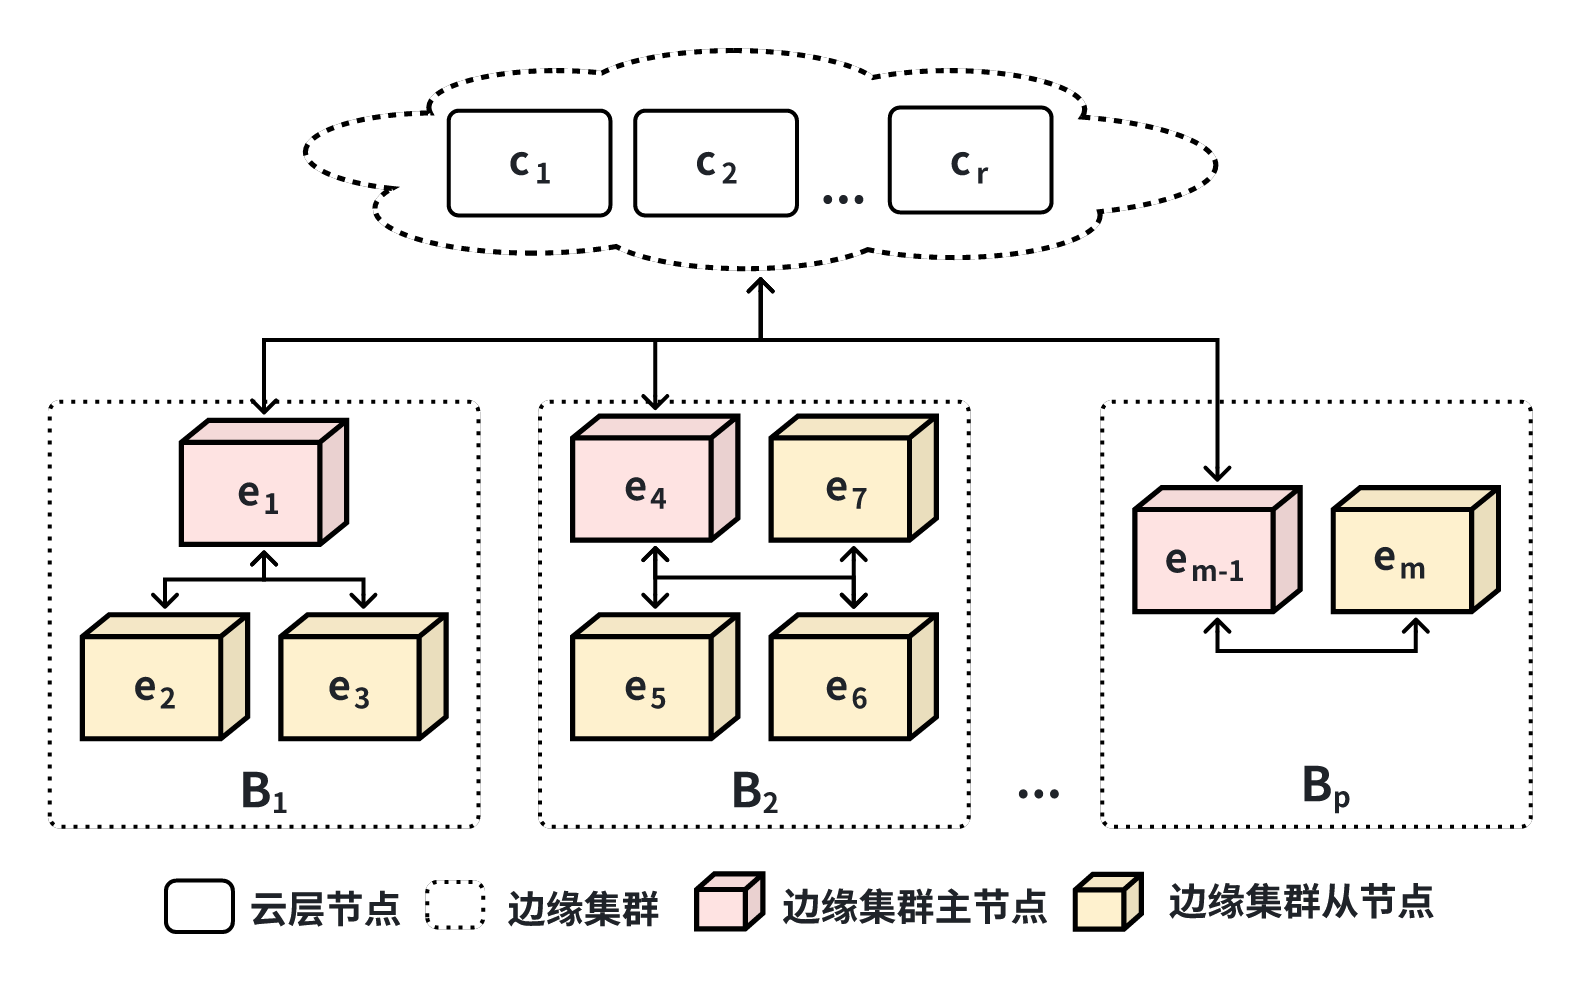
\includegraphics[width=0.8\linewidth]{pics/3-5边缘集群.png}
  \caption{主从结构的边缘集群概览}
  \label{fig:3-5edgecluster}
\end{figure}

主节点作为边缘集群的核心组件,其主要职责包括元数据管理、跨层通信以及集群内部的任务调度。首先,主节点维护并同步边缘集群的元数据,这些元数据分为两类:静态资源状态和运行状态。静态资源状态则描述了集群的固有能力,涵盖各节点的资源供给情况、计算能力;运行状态反映集群的动态行为,包括各节点负载的实时计算队列、节点健康状态等动态信息。主节点通过定期与云端通信,将上述元数据上传至云端,为云端进行全局调度决策提供依据。此外,主节点还负责集群内部的任务调度。当某个边缘节点因资源不足或故障而无法支持特定任务时,主节点会基于当前集群内部状态,在其他具备适配资源的节点中寻找最优候选者完成任务分配。

根据边缘集群的架构设计与主节点的功能特性,为了更清晰地描述边缘集群的组成结构及其运行机制,本文引入了边缘集群的形式化定义。

\paragraph{定义3.8 (边缘集群)} 边缘集群$B_k \in \mathcal{B}$可表示为一个 3 元组:
\[
B_k = (L_k, \mathcal{E}_k, \Phi_k)
\]
其中:
\begin{itemize}
    \item $L_k$表示主节点,属于计算节点集合$\mathcal{E}$的特殊元素,承担集群协调者的角色。
    \item $\mathcal{E}_k = \{e_{kj}\}_{j=1}^{m_k} \subseteq \mathcal{E}$表示隶属本集群的边缘节点集合,且$L_k \equiv e_{k1} \in \mathcal{E}_k$,即主节点$L_k$也被视为该集合中的一个节点,用$e_{k1}$表示。
    \item $\mathcal{W}_k = (\Psi_k, \Gamma_k)$ 表示内部网络拓扑参数。其中,$\Psi_k = [\psi_{jj'}^{(k)}] \in \mathbb{R}^{m_k \times m_k}$ 为时延矩阵,$\psi_{jj'}^{(k)}$表示节点$e_{kj}$到$e_{kj'}$的单向传输时延;$\Gamma_k = [\gamma_{jj'}^{(k)}] \in \mathbb{R}^{m_k \times m_k}$ 为带宽矩阵,$\gamma_{jj'}^{(k)}$表示节点$e_{kj}$到$e_{kj'}$的可用带宽
\end{itemize}


在云边协同架构中,调度器的核心目标是将终端设备产生的流式数据高效地分流至适配的计算节点上进行处理。然而,这种调度面临显著挑战:边缘集群内部具备高带宽、低延时的通信特性,而边缘集群间或云边之间的通信则表现出高延时、低带宽的特点。因此,调度策略需要兼顾局部响应效率与全局资源优化,这对传统集中式调度机制提出了严峻考验。本文提出一种基于计算资源层级化管理的动态任务分配机制,旨在通过多级调度器的协作优化AI推理任务的执行效率与资源利用率。

\begin{figure}[h]
  \centering
  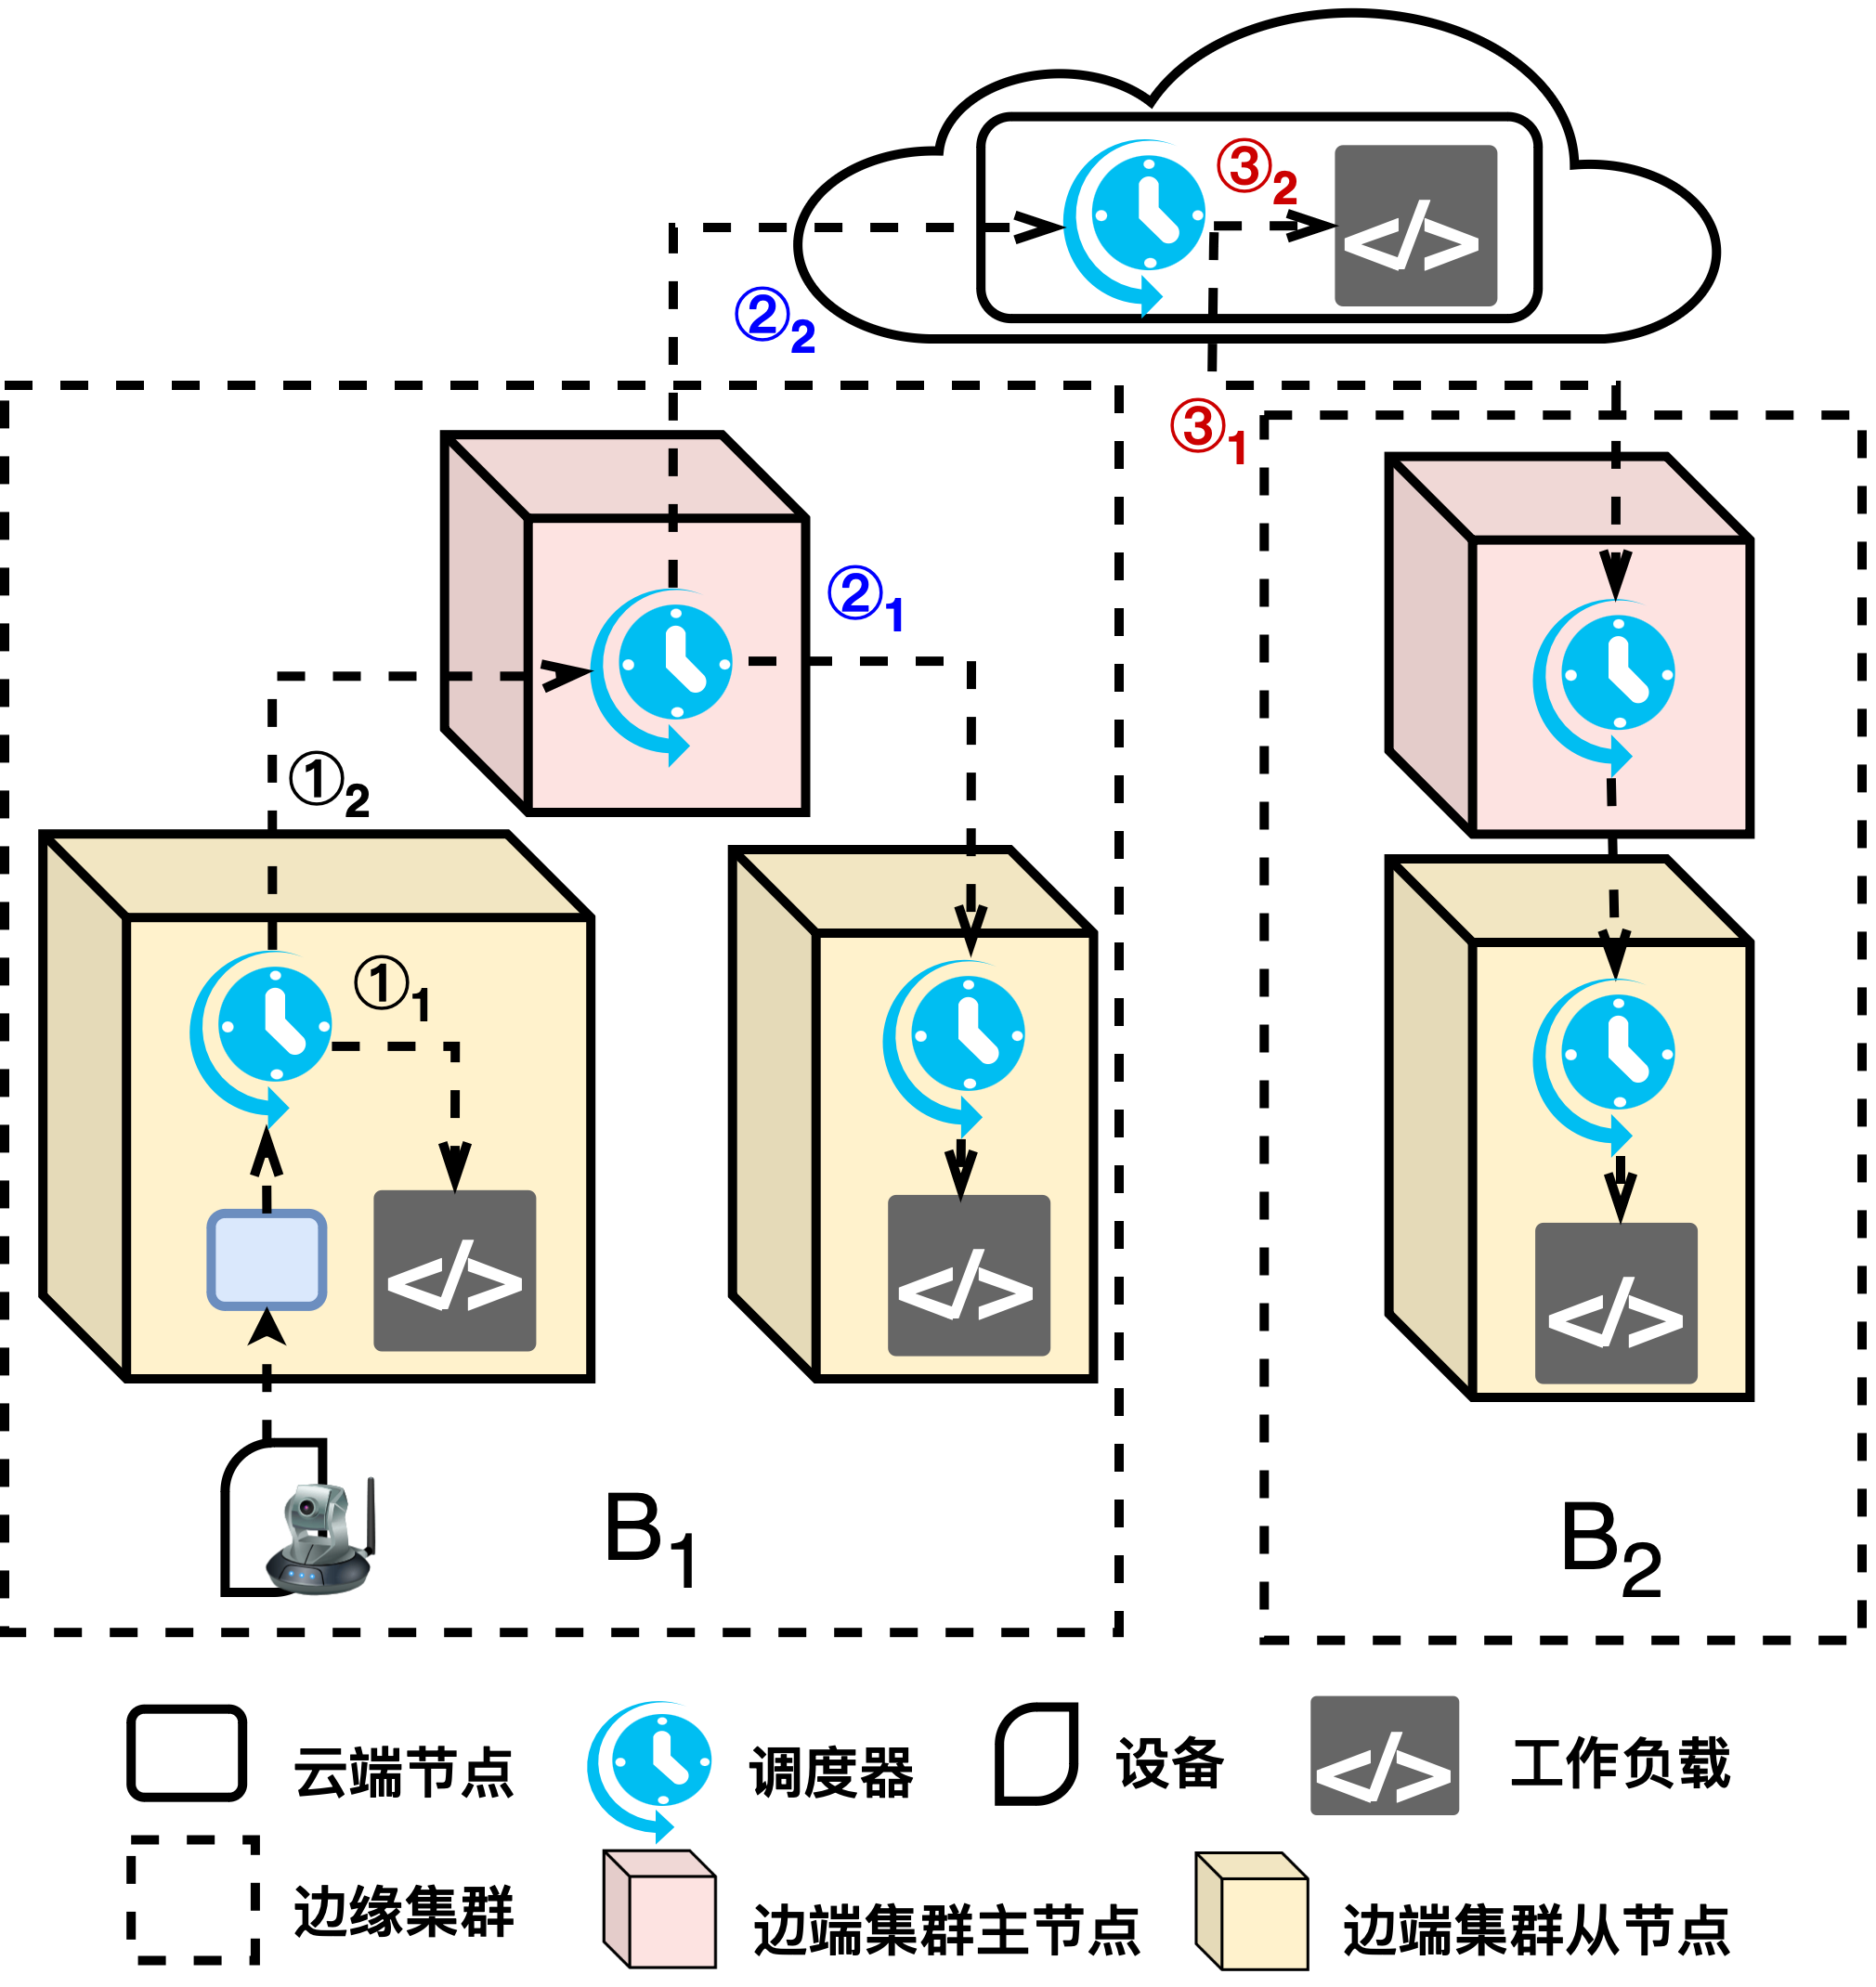
\includegraphics[width=0.6\linewidth]{pics/3-6调度器.png}
  \caption{多级调度器协作示意图}
  \label{fig:3-6scheduler}
\end{figure}

如图\ref{fig:3-6scheduler}所示,分层调度框架采用三级协同决策机制,其核心调度流程如下:当终端设备生成数据流时,框架首先尝试将终端设备产生的数据流在本地计算节点内完成处理;若本地计算节点无法满足AI负载实例 $\ell_s$ 的部署需求(例如,缺乏适配的硬件架构支持或资源供给不足),或者本地计算队列 $\mathcal{Q}_s^j(t_\omega)$ 的容量已饱和,则将任务转发至所属边缘集群进行进一步调度;若边缘集群内的所有计算队列均已达到容量上限,任务最终会被提交至云端全局调度器,以利用跨集群或云端资源实现动态分配。(修改这一段,使得表述更加自然,更具有逻辑)



\begin{figure}[h]
  \centering
  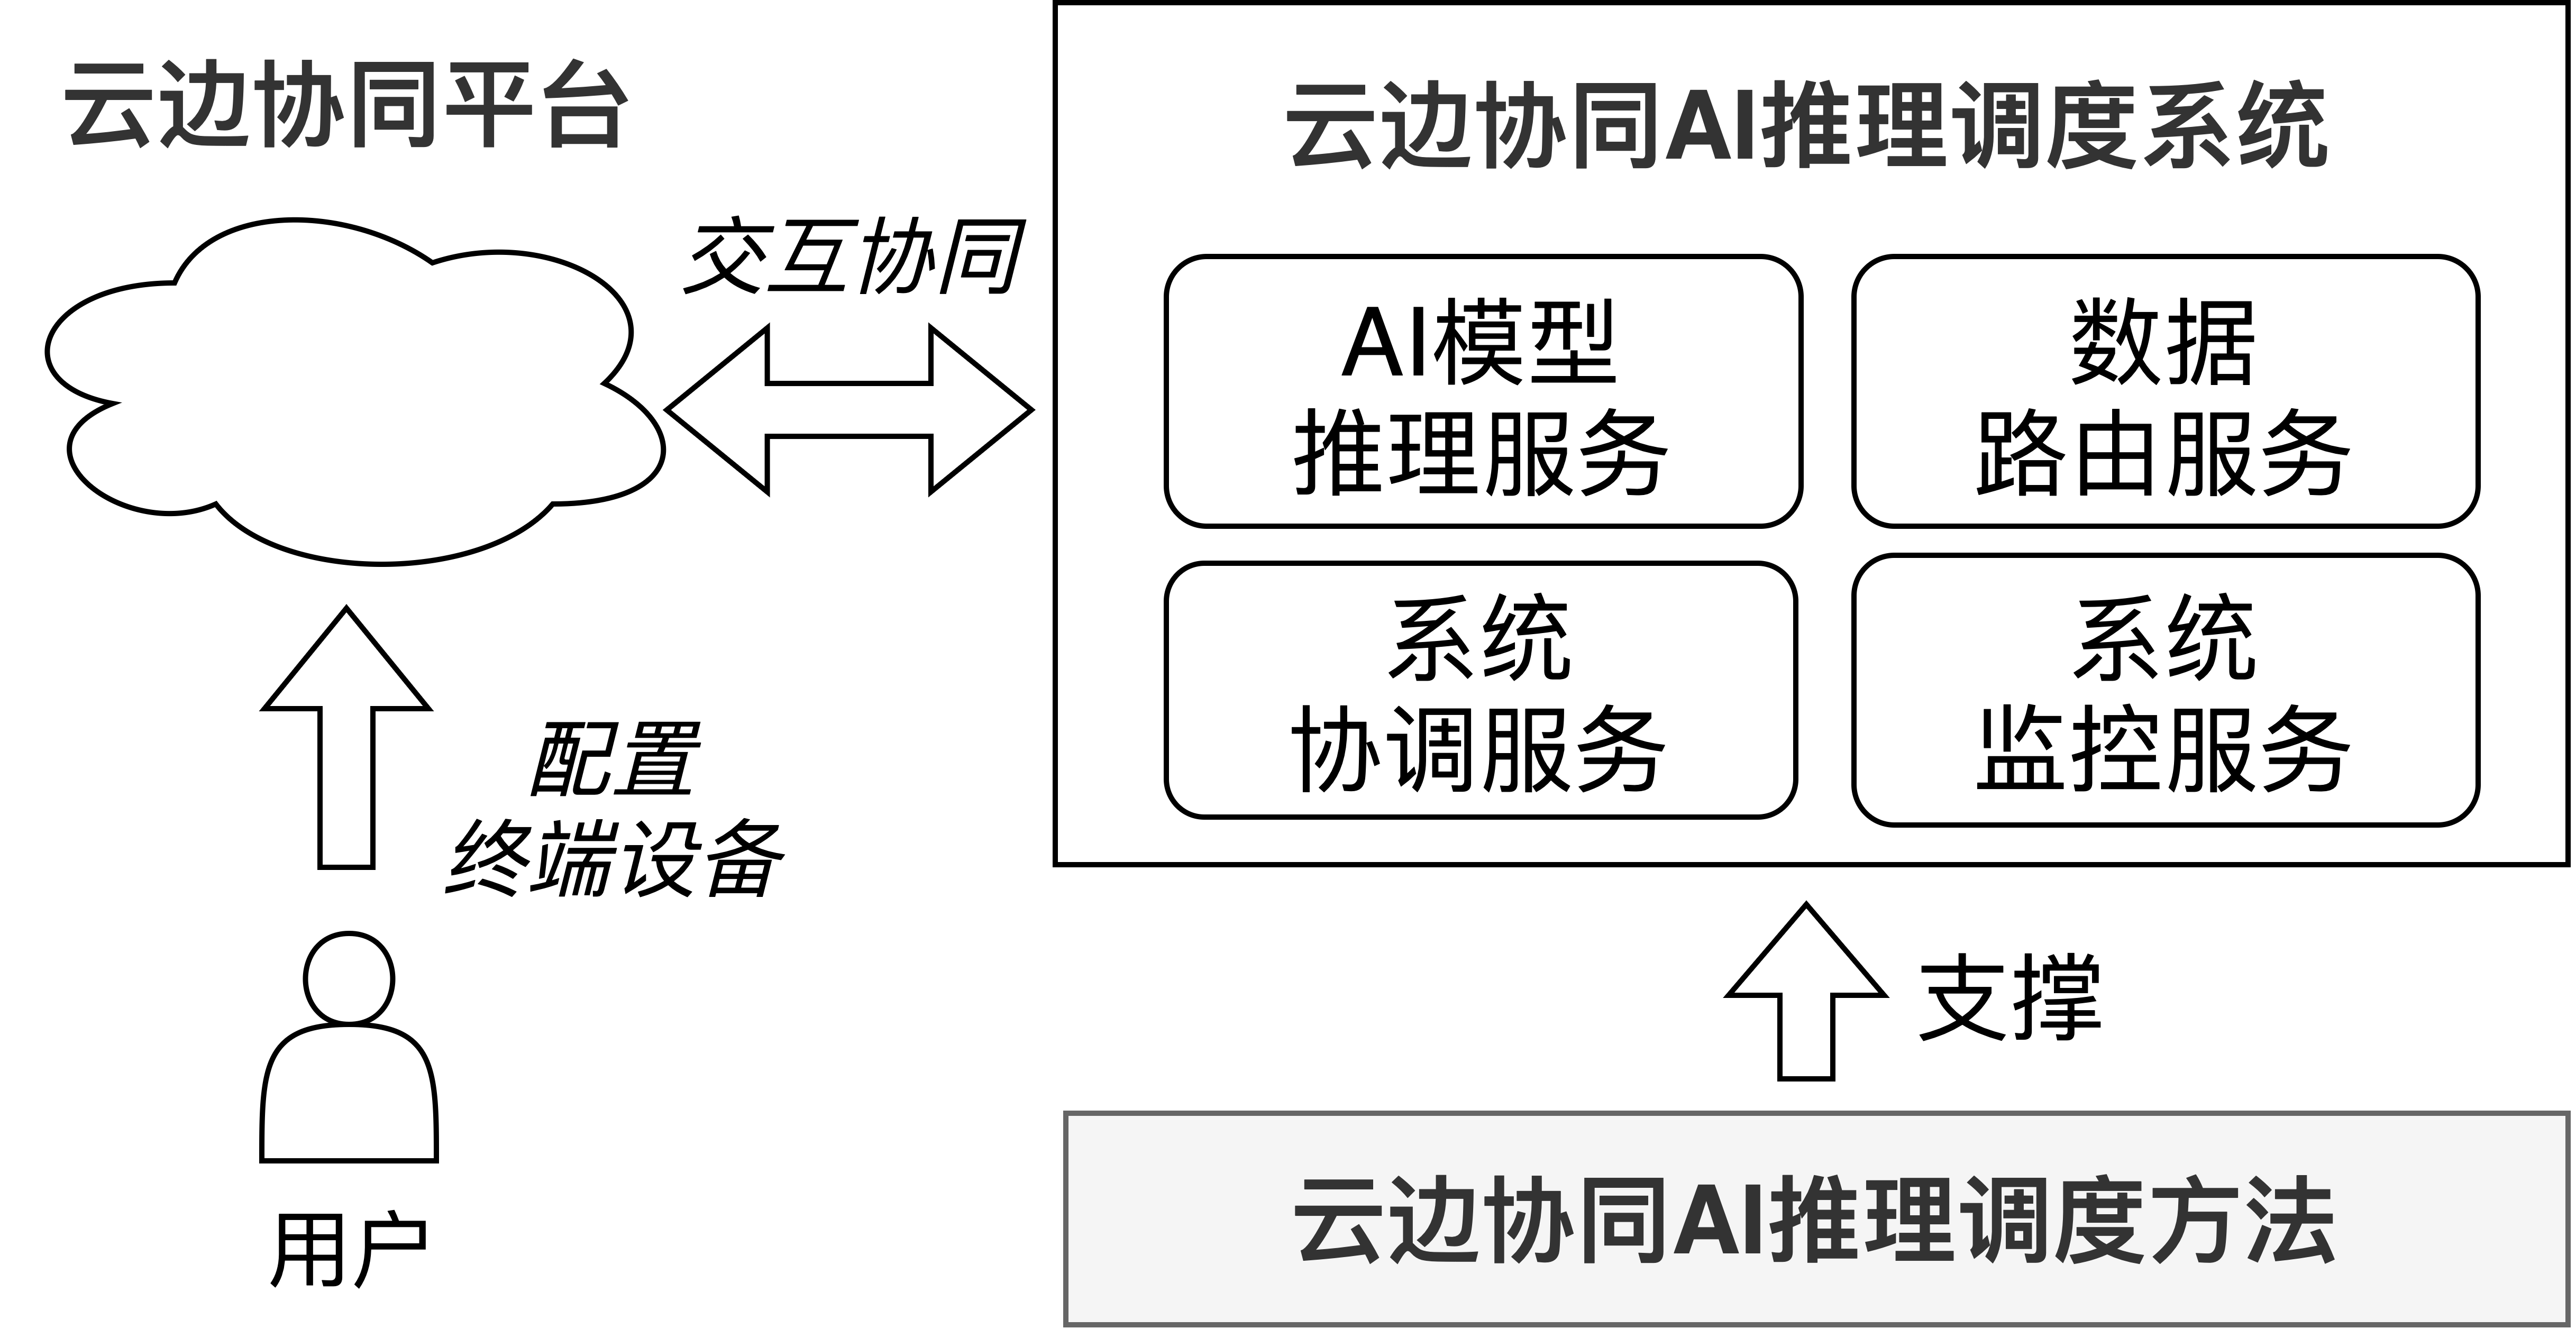
\includegraphics[width=0.7\linewidth]{pics/3-all.png}
  \caption{云边协同AI推理调度方案KEAS示意图}
  \label{fig:3-all}
\end{figure}

图\ref{fig:3-all}展示了本文提出的云边协同AI推理调度方案KEAS的整体架构。该方案涉及用户、云边协同平台、云边协同AI推理调度方法和系统等多个角色。在运行时,用户通过云边协同平台配置终端设备,这些设备会持续采集并生成流式时序数据。系统与云边协同平台保持实时交互,动态监测终端设备的状态信息,并结合边缘和云端的资源情况,动态调度流式时序数据的AI推理请求。通过边缘节点间的水平协作以及云端全局的垂直协同,该方案实现了资源的高效利用与任务的优化分配。

\begin{figure}[ht]
  \centering
  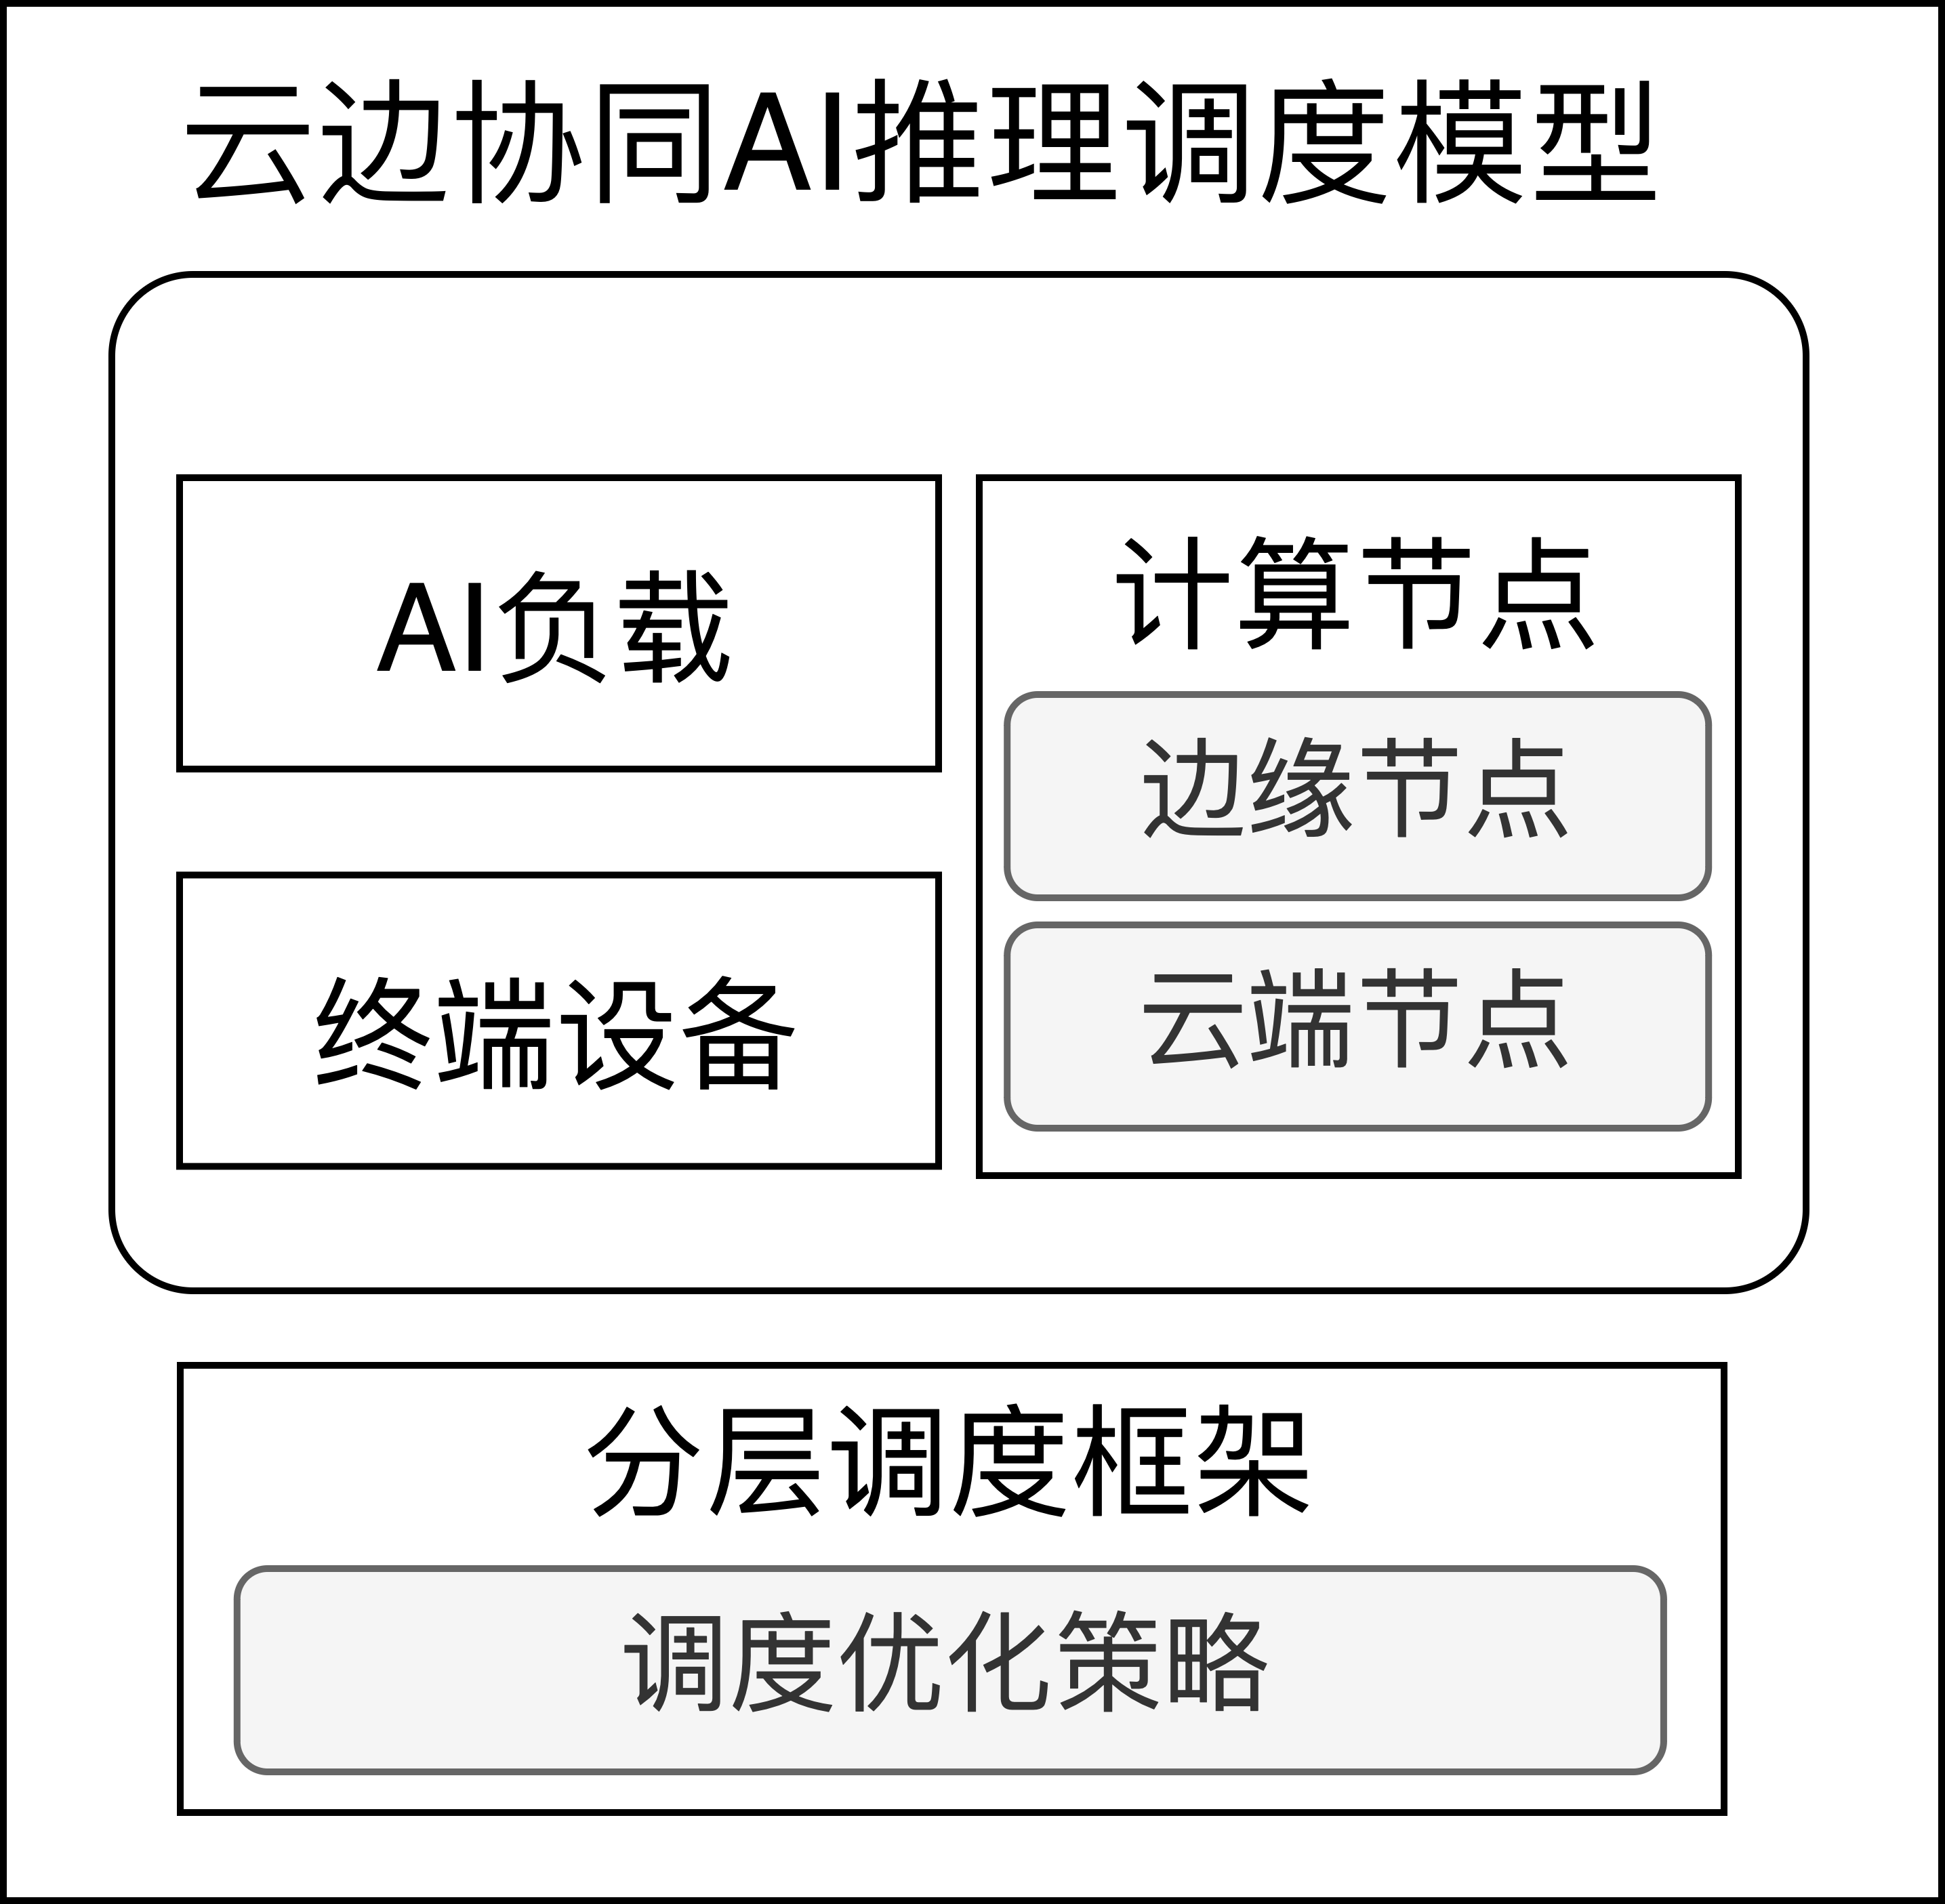
\includegraphics[width=0.4\linewidth]{pics/3-0架构.png}
  \caption{云边协同AI推理调度方法架构示意图}
  \label{fig:3-0arch}
\end{figure}

图\ref{fig:3-0arch}展示了方法的基本架构。该架构基于云边协同AI推理调度模型构建,清晰界定了云边平台的核心组件,包括终端设备、AI负载实例、计算节点、边缘集群及分层调度框架。同时,该模型详细定义了流式数据调度机制的关键要素,例如数据分流策略和各级调度器在运行时可见的状态信息等。基于此理论模型,本文提出了分层调度体系,其核心内容如下:

\begin{enumerate}
    \item \textbf{云边协同AI推理调度模型}:本文构建了形式化的云边协同AI推理调度模型,系统定义了终端设备、AI负载实例、计算节点等核心组件及其交互机制。通过引入计算队列状态感知和数据流驱动的动态调度框架,建立了覆盖边缘节点、集群到云端的多层级优化模型,为分层调度策略的设计奠定了理论基础。
    \item \textbf{云边协同AI推理分层调度策略}:本文提出分层调度架构。其中,本地调度策略以节点级资源最优分配为目标,通过动态调整分流比例优先保障直连设备服务质量,最小化跨节点传输开销;中间层次调度结合时延敏感度感知机制,构建多维度优先级队列,确保在满足时延约束的同时最大化集群内部资源利用率;云端全局调度策略构建跨域资源协调机制,采用最短任务先调度方法,减少碎片。
\end{enumerate}



\subsection{设备直连节点本地调度}

\begin{figure}[h]
  \centering
  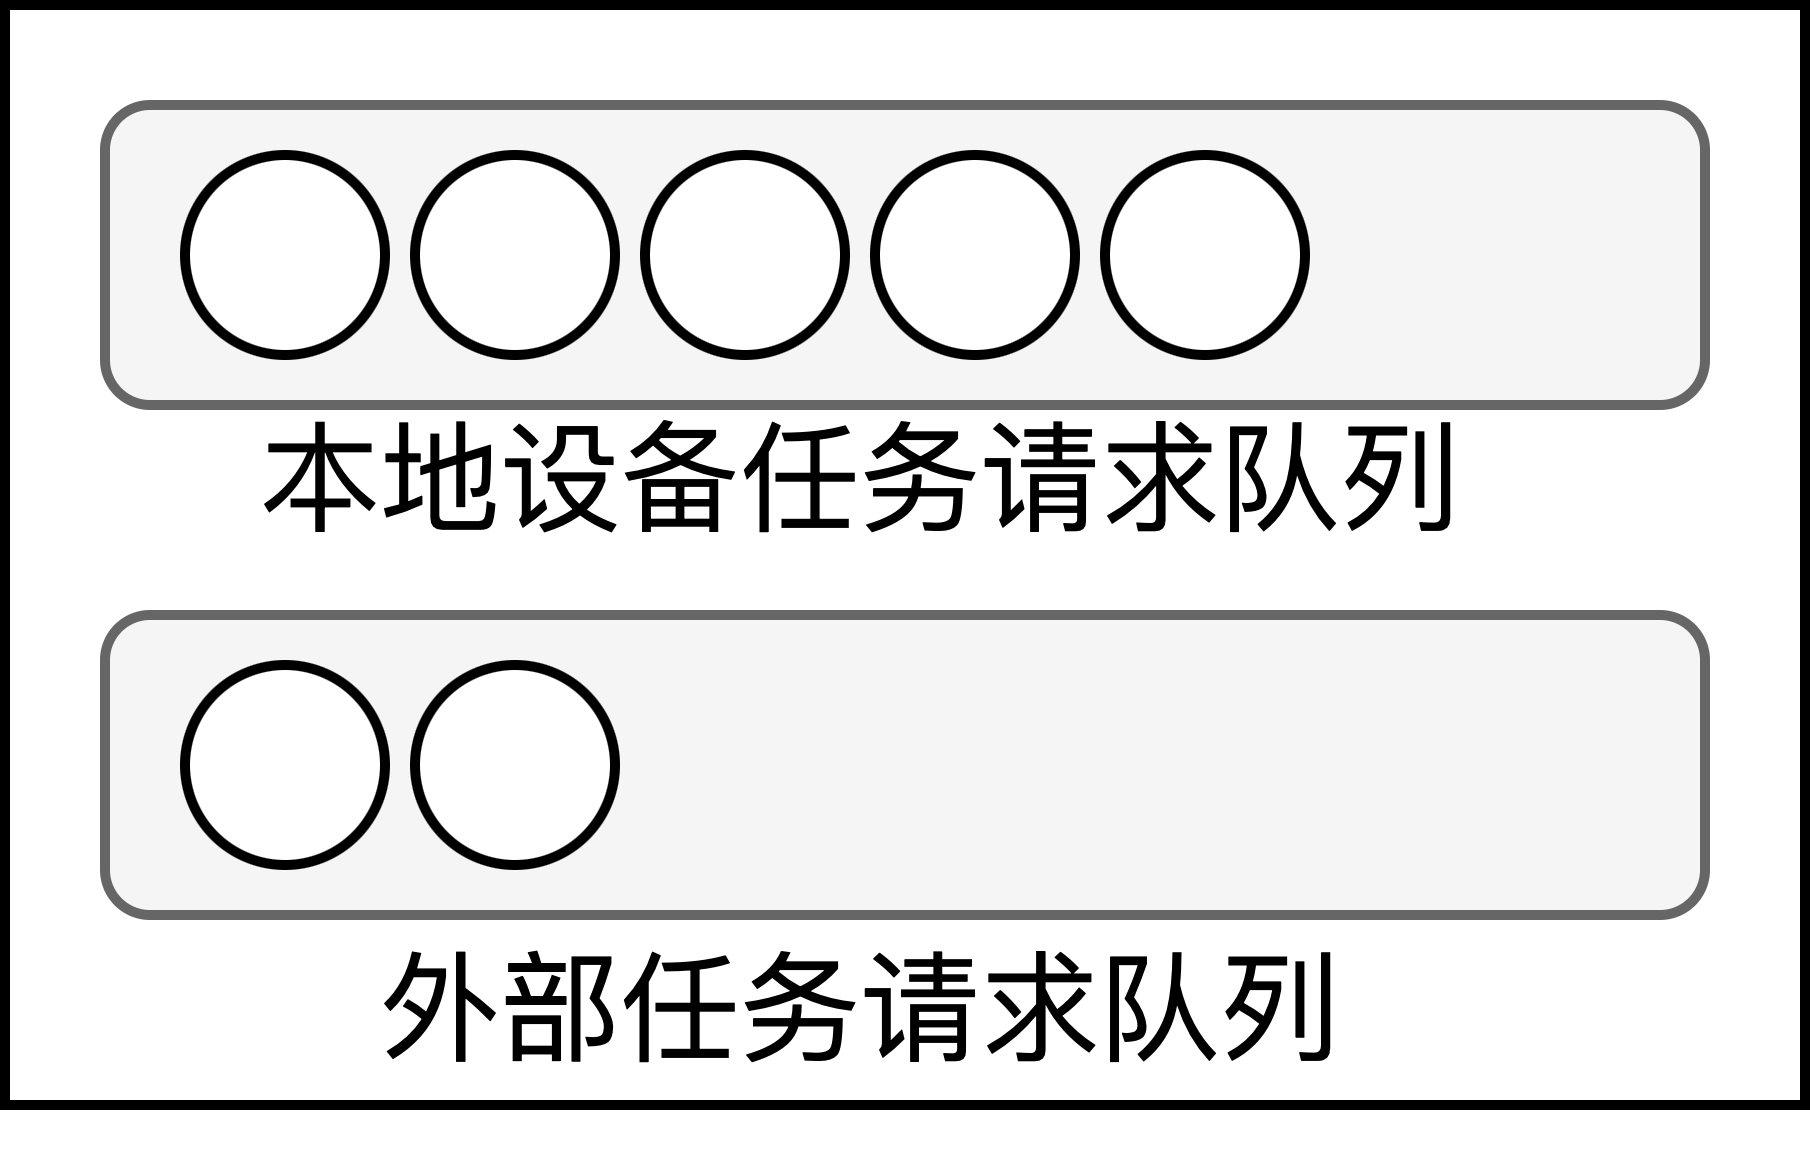
\includegraphics[width=0.4\linewidth]{pics/3-10本地调度.png}
  \caption{设备直连节点本地调度任务队列}
  \label{fig:3-10local}
\end{figure}

对于设备直连节点,本地存在两个任务队列:一个是本地设备的任务队列,另一个是上级节点分配的任务队列,如图\ref{fig:3-10local}所示。本地节点的调度器优先调度本地设备的任务请求,然后调度上级节点分配的任务请求。为了最小化外部流量,调度器首先处理单次采集量$\varsigma_\beta$ 最大的任务。

本文提出基于贪心策略的本地调度算法。该算法通过构建优先级队列,以本地设备单次数据采集量$\varsigma_{i\beta}$为依据,确保本地设备的数据流能够优先获得调度资源,同时有效减少跨节点传输的开销。在此基础上,算法还引入了弹性容量分配机制,在严格满足计算队列容量约束的前提下,动态调整数据分流比例。这一机制不仅能够保障本地服务质量,还能最大化系统吞吐量,从而在资源利用与性能需求之间实现平衡。具体算法流程如算法\ref{alg:local_scheduling}所示。

\begin{algorithm}[ht]
\caption{本地调度算法}
\label{alg:local_scheduling}
\begin{algorithmic}[1]
\REQUIRE  
  直连设备集合$\mathcal{D}_j$,  节点$v_j$在$t_\omega$时间窗的计算容量$C^{t_\omega}_j$, 设备流式数据特征元组$\{(g_i^{t_\omega}, \varsigma_{i\beta})\}_{d_i \in \mathcal{D}_j}$
\ENSURE  
  设备到节点的分流比例集合$\{z_{ij}^{t_\omega}\}$

\STATE 初始化分流比例 $z_{ij}^{t_\omega} \leftarrow 0,\ \forall d_i \in \mathcal{D}_j$  
\STATE 剩余可用容量 $R \leftarrow C_j^{t_\omega}$  

\STATE 生成设备优先级队列 $\mathcal{P} \leftarrow \textsc{Sort}(\mathcal{D}_j, \varsigma_{i\beta} \downarrow)$  
  \COMMENT{按单次数据量$\varsigma_{i\beta}$降序排序}

\WHILE{$\mathcal{P} \neq \emptyset$ \AND $R > 0$}
  \STATE 取出队首设备 $d_i \leftarrow \mathcal{P}.\textsc{Dequeue}()$
  \STATE 计算资源需求 $u_i \leftarrow g_i^{t_\omega} \times \varsigma_{i\beta}$ 
  
  \IF{$u_i \leq R$}
    \STATE $z_{ij}^{t_\omega} \leftarrow 1.0$ \COMMENT{全量本地化处理}
    \STATE $R \leftarrow R - u_i$ \COMMENT{更新剩余容量}
  \ELSE
    \STATE $z_{ij}^{t_\omega} \leftarrow R / u_i$ \COMMENT{按比例分配剩余容量}
    \STATE $R \leftarrow 0$ \COMMENT{触发资源耗尽状态}
  \ENDIF
\ENDWHILE
\RETURN $\{z_{ij}^{t_\omega}\}_{d_i \in \mathcal{D}_j}$
\end{algorithmic}
\end{algorithm}

算法\ref{alg:local_scheduling}的总体时间复杂度为$O(|\mathcal{D}_j| \log |\mathcal{D}_j|)$,其中通过排序函数 $\textsc{Sort}$ 构建设备优先级队列 $\mathcal{P}$的时间复杂度为 $O(|\mathcal{D}_j| \log |\mathcal{D}_j|)$,主循环逐一处理优先级队列中的设备的时间复杂度为 $O(|\mathcal{D}_j|)$。

\subsection{中间层次与云端全局调度}

\begin{figure}[h]
  \centering
  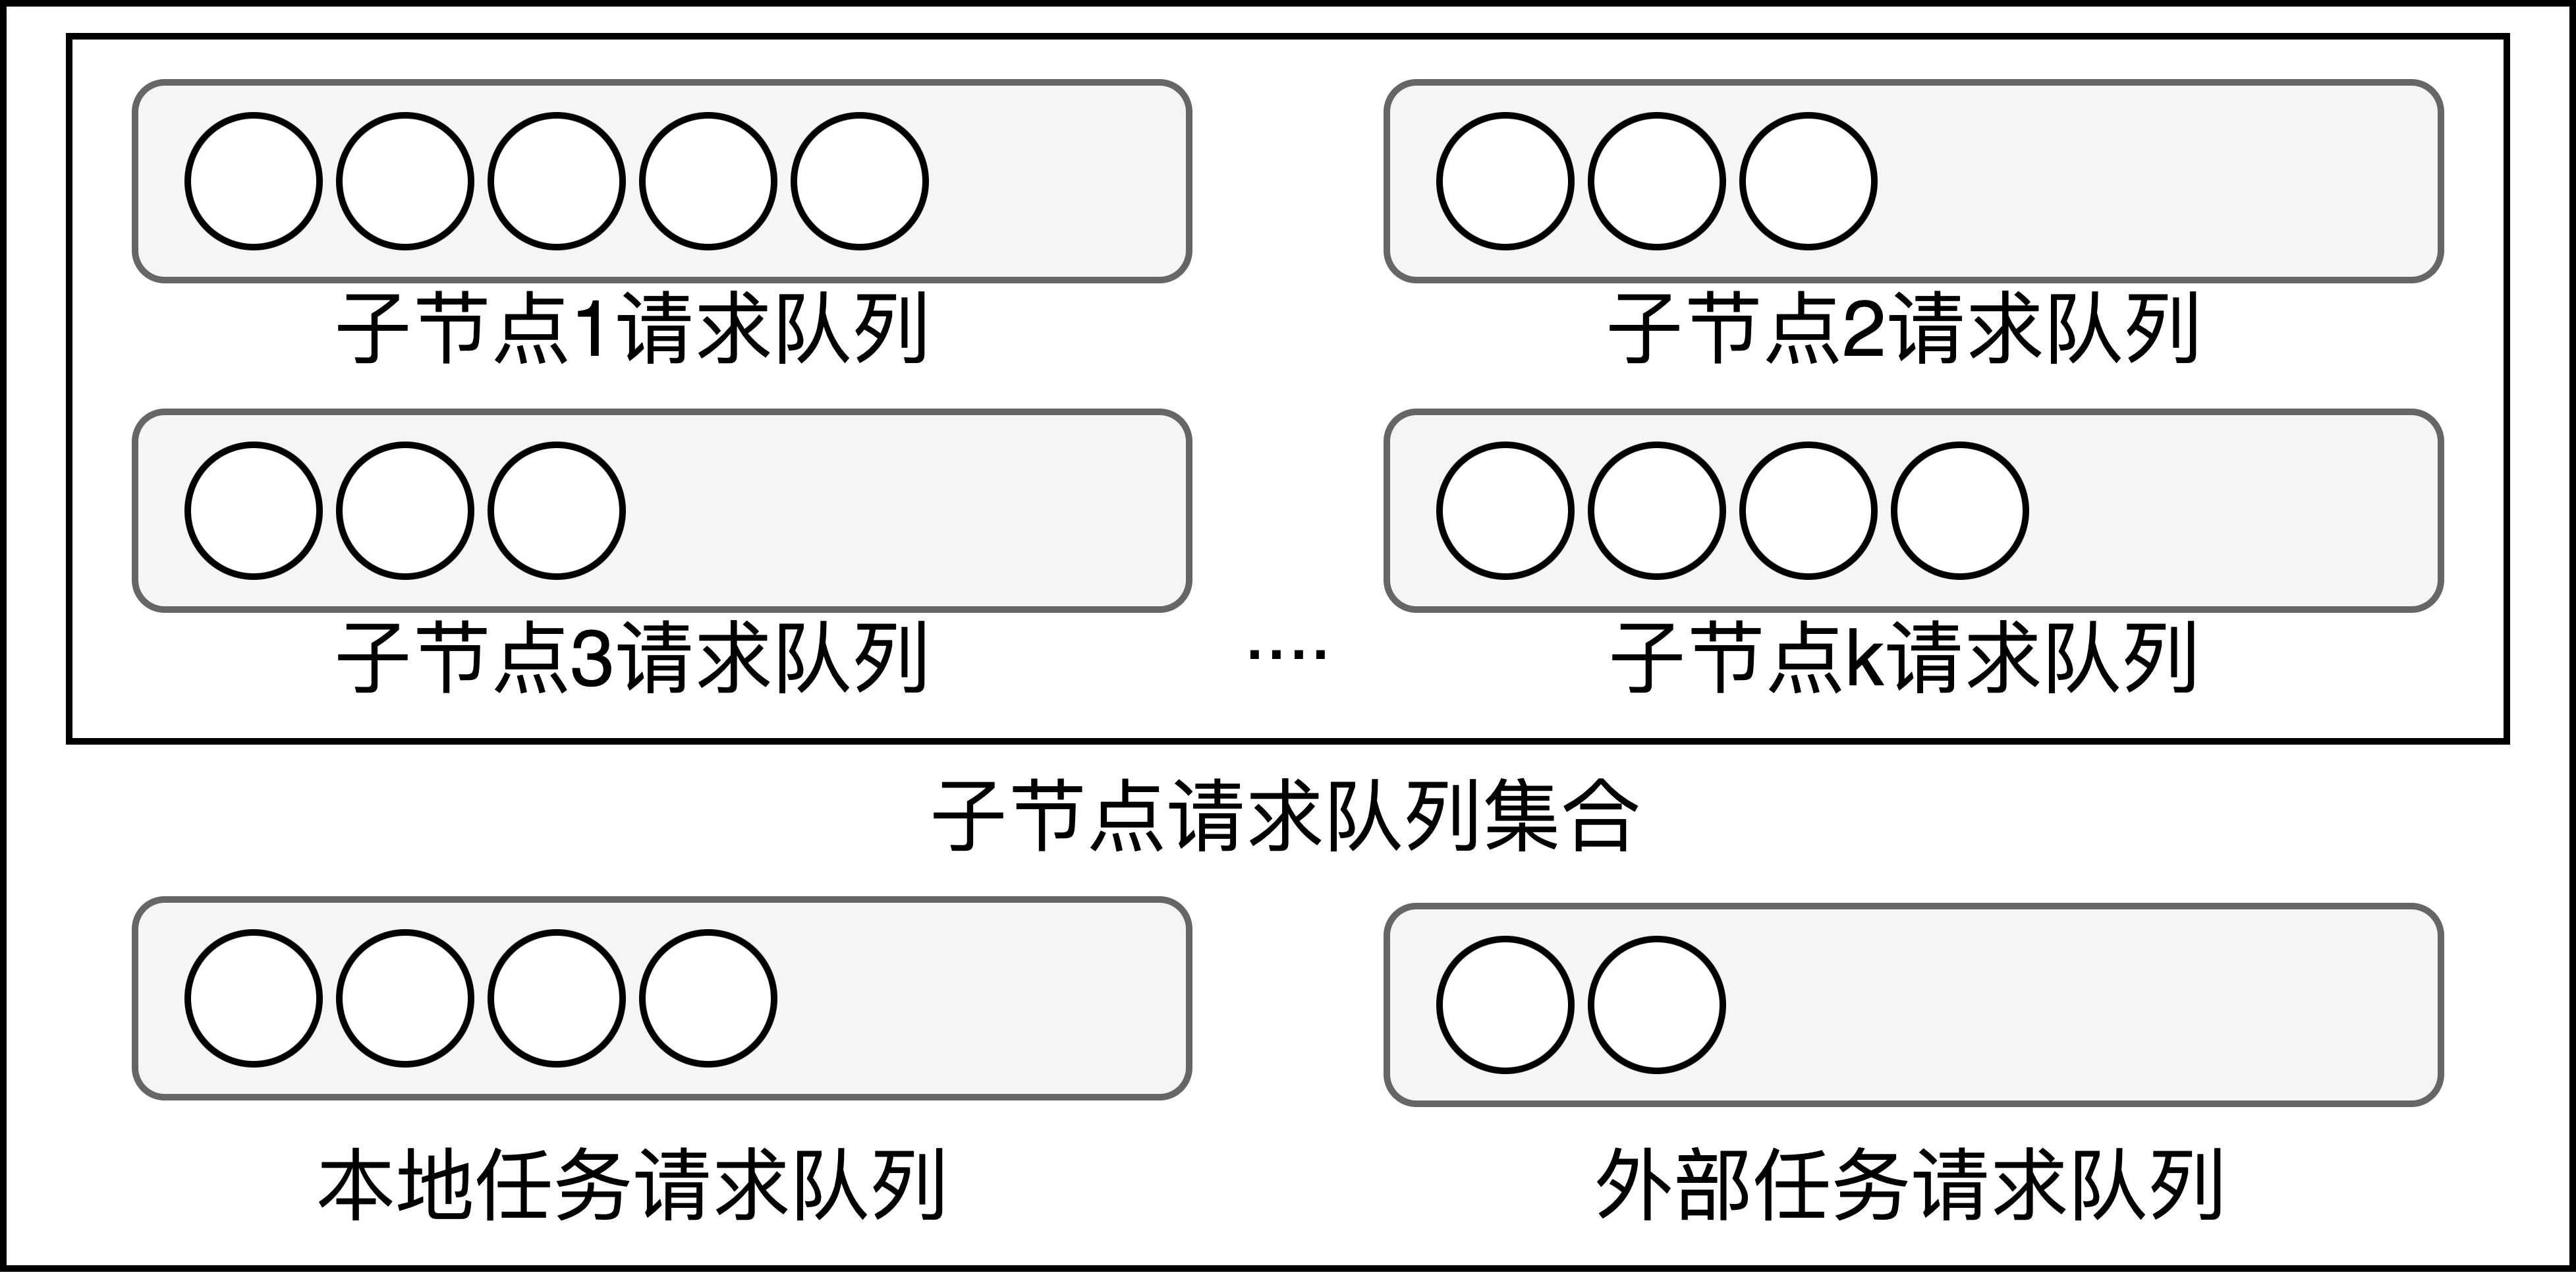
\includegraphics[width=0.8\linewidth]{pics/3-11集群调度.png}
  \caption{上层节点调度任务队列}
  \label{fig:3-11cluster}
\end{figure}

在每一级中间层次的节点中,都会维护其所有子节点的任务队列信息,同时记录自身的任务队列以及外部节点的任务队列信息。当某个设备的任务请求在下一级节点未能成功调度时,该请求会在当前层次的节点进行调度处理,如图\ref{fig:3-11cluster}所示。这种机制确保了任务能够在合适的节点层级得到及时响应,从而提高了系统的整体调度效率。为了最小化外部流量,中间层次调度器首先处理单次采集量$\varsigma_\beta$ 最大的任务。而云端为了实现最大化设备处理,可以优先处理最小的碎片任务,从而保证尽可能多的设备请求数据被完整处理。

本文提出了一种结合贪心策略与多维度优先级队列的中间层次与上层调度算法。该算法首先根据设备单次数据采集量或剩余数据量对流式数据进行优先级排序,构建初始优先级队列,在此基础上,针对每条流式数据,算法筛选出集群中具有剩余计算队列容量的候选节点,并进一步依据端到端时延建立时延优先队列。通过引入时延敏感度感知机制,算法有效降低了集群内部调度的总时延,同时满足任务的时延约束要求。此外,算法采用动态分配策略,在候选节点间按剩余容量比例分配数据流,既避免了单一节点过载问题,又最大化了集群内部计算资源的利用率。通过这一机制,算法在保证服务质量的同时实现了高效的资源调度与任务分配,具体流程详见算法\ref{alg:cluster_scheduling}。

\section{方法概述}

\begin{figure}[h]
  \centering
  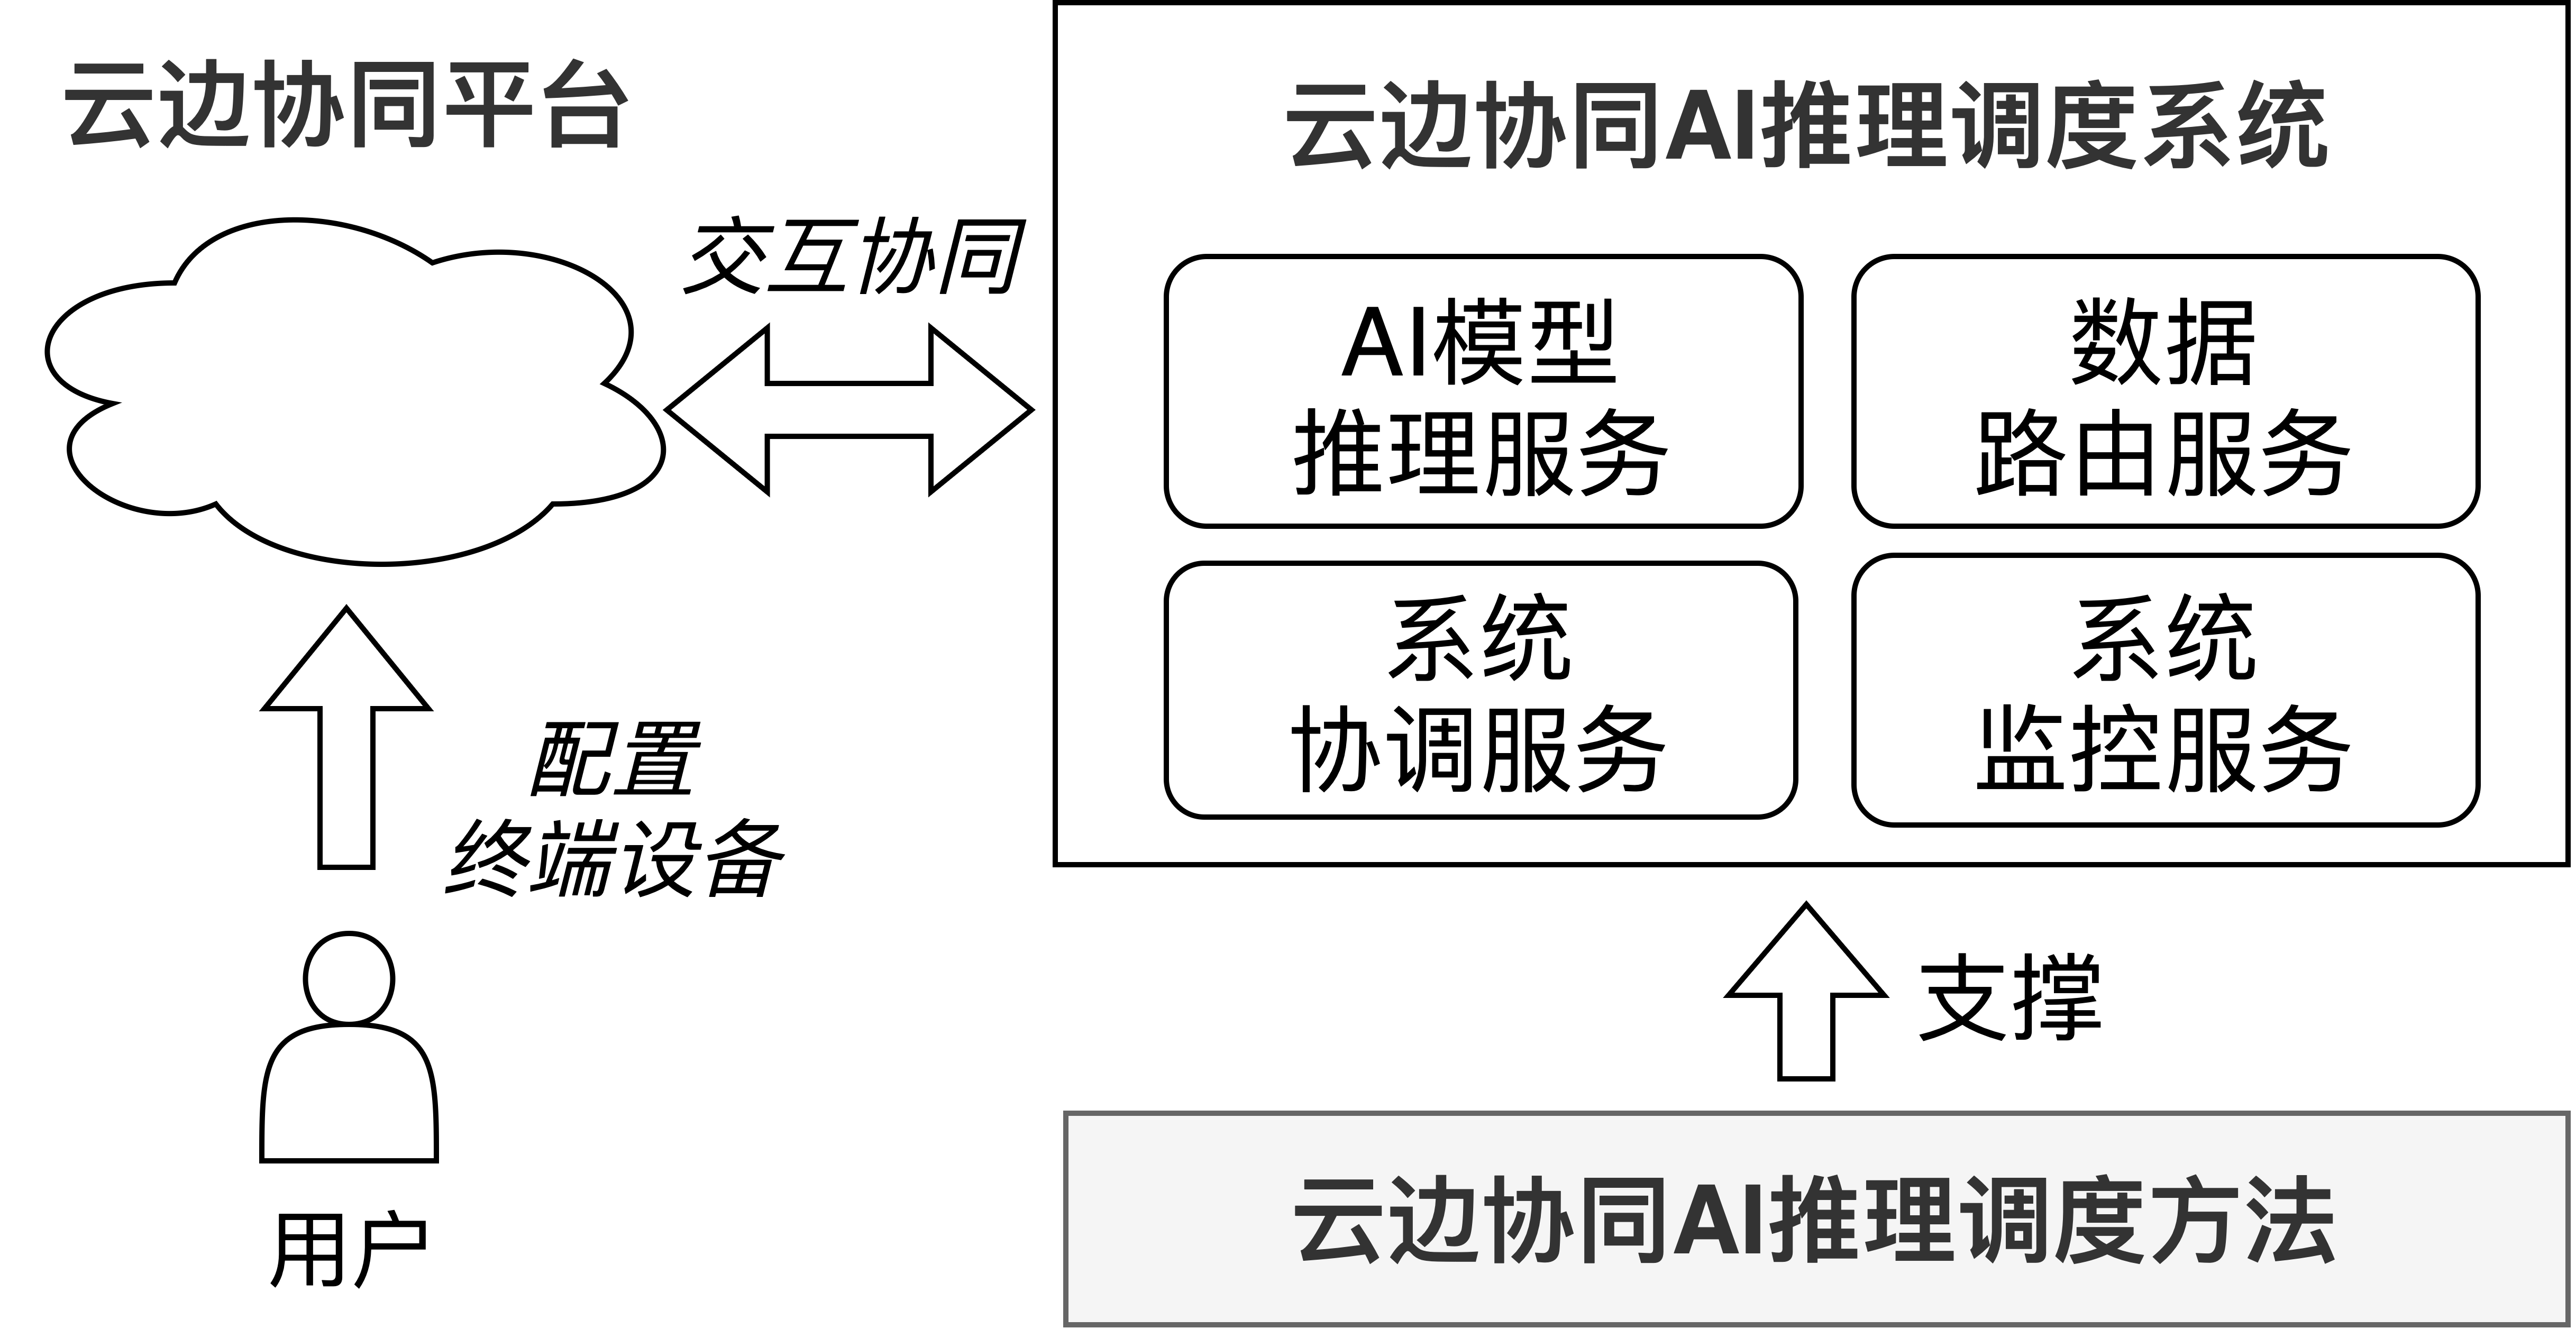
\includegraphics[width=0.7\linewidth]{pics/3-all.png}
  \caption{云边协同AI推理调度方案KEAS示意图}
  \label{fig:3-all}
\end{figure}

图\ref{fig:3-all}展示了本文提出的云边协同AI推理调度方案KEAS的整体架构。该方案涉及用户、云边协同平台、云边协同AI推理调度方法和系统等多个角色。在运行时,用户通过云边协同平台配置终端设备,这些设备会持续采集并生成流式时序数据。系统与云边协同平台保持实时交互,动态监测终端设备的状态信息,并结合边缘和云端的资源情况,动态调度流式时序数据的AI推理请求。通过边缘节点间的水平协作以及云端全局的垂直协同,该方案实现了资源的高效利用与任务的优化分配。

本节从系统架构、任务特性与执行机制三个维度展开论述。首先剖析云边协同的物理拓扑与逻辑分层,继而阐述AI推理任务的执行流程与适配挑战,最后通过分层调度策略实现资源动态优化。




\subsubsection{边缘主节点调度实验分析}

\begin{figure}[ht]
  \centering
  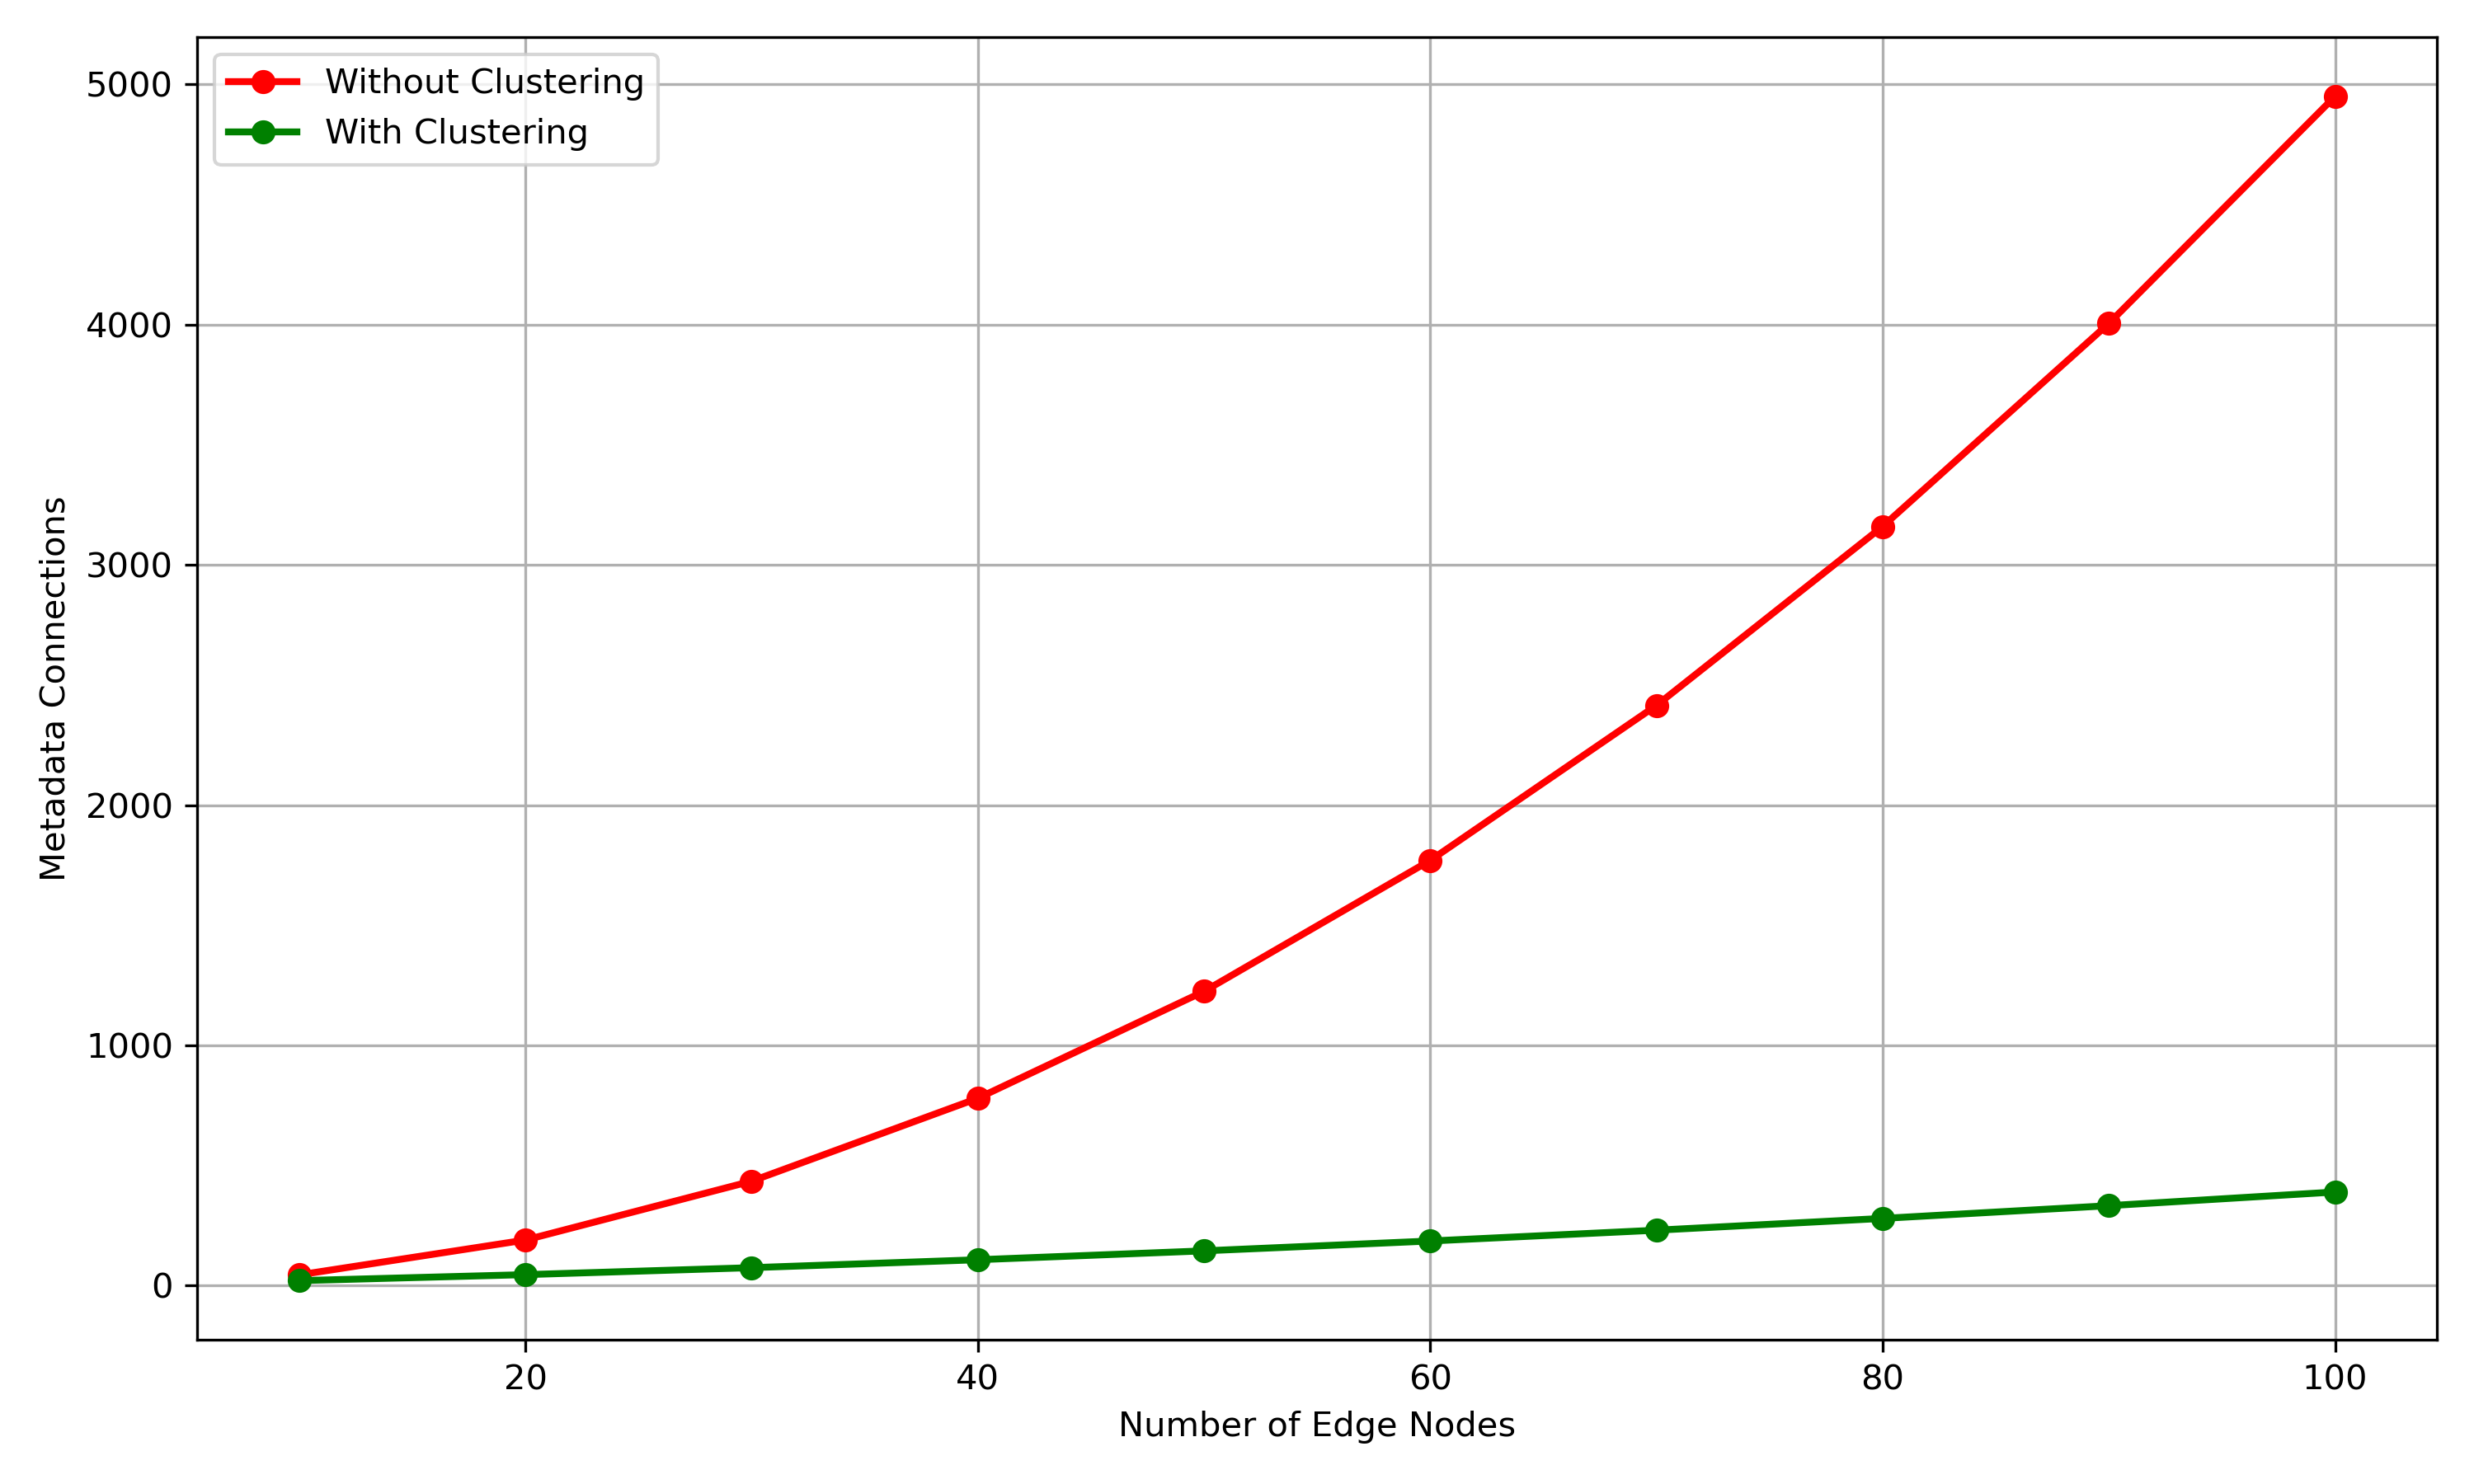
\includegraphics[width=0.8\linewidth]{pics/expr/metadata_connections_comparison.png}
  \caption{引入中间层次后前后元数据交互规模的对比}
  \label{fig:exp5}
\end{figure}

在云边协同系统中,随着边缘节点数量增加,云端需要维护的元数据交换链路规模迅速膨胀,导致网络负载增加和带宽利用率下降,严重影响系统效率。为解决这一问题,本文将云边端三层物理拓扑抽象为树状拓扑,将边缘节点划分为若干子树,显著降低元数据交换复杂度,并通过分级调度策略减少云边交互频率。如图\ref{fig:exp5}所示,该方法有效提升了系统的响应速度和资源利用率。

最后,系统性能评估实验深入分析了分层调度决策对资源利用率的影响。通过监测批处理任务的运行情况,实验间接验证了调度算法在负载均衡方面的有效性。结果表明,分层调度策略能够根据各计算节点的实时负载状态动态分配任务,从而在不同节点间实现任务负载的合理分布。